\chapter{Handling of trimuon correlations at LHCb}
\label{chap:trimuon}

\textit{Having three muons passing through the detector may result in few issues, which need to be addressed. Two collimated muons may cross through the same parts of the detector if they bear the same charge, which causes problems in resolving their individual tracks. Hence, from the tracking point of view, ghosts and clones are much more likely to occur. In LHCb, plethora of muon \Gls{PID} variables can be used to suppress these types of spurious tracks, however, one must be careful once estimating the relevant \gls{PID} efficiencies as most efficiencies will be dependant on number of muons in the detector.}

\section{Muon PID variables \mybox{ULRIK}}
There is a further set of muon variables apart from the ones mentioned in \autoref{muonID} that are available for \gls{PID} of muon. In this section summary of the variables used in analysis of \Bmumumu is discussed.

\subsection{Binary Muon PID variables \mybox{ULRIK}}
Similar to \texttt{isMuon} shown in \autoref{tab:ismuontab}, there are two more binary variables, \texttt{isMuonTight} and \texttt{isMuonLoose}, that can help with classification of muons. As their name suggests, \texttt{isMuonLoose} has weaker and \texttt{isMuonTight} has stronger conditions to satisfy as compared to \texttt{isMuon}. 

In each muon station (\gls{muonstation}) and in each dimension in perpendicular plane ($d=\{x,y\}$), \gls{FOI} is defined as a function of momentum $p$  in a following way:
\begin{equation}
	FOI_{d}=\rho_{d,1}+\rho_{d,2}\cdot \exp \left(\frac{\rho_{d,3}\cdot p}{\gevc} \right).
\end{equation}

Muon passing through the detector will leave hit in $pad_{d}$ of each muon station and therefore have $h_{d}$ coordinate. Extrapolation coordinates from tracking system made into the stations are denoted $E_{d}$. The hits are considered to be within the \gls{FOI} for given $d$ if they satisfy the condition that $|| h_{d} - E_{d} || < FOI_{d} \cdot pad_{d}$. 

The detector information is read out in $x$ and $y$ direction separately. The pad slicing according to this read-out scheme is known as \textit{physical} slicing of pads. However, as seen in \autoref{fig:pads}, the overlapping $x$ and $y$ \textit{physical} pads of can be grouped into \textit{logical} pads, which give information about $x$ and $y$ simultaneously. These leads to two groups of hits according to pad type: uncrossed hits - registered within \textit{physical} pads only and crossed hits - given by \textit{logical} pads. Whereas \texttt{isMuon} only requires positive decision from uncrossed hits, \texttt{isMuonTight} requires positive decision based on crossed hits. 


\begin{figure}[!h]
        \centering
        %
\includegraphics[width = 0.3\textwidth]{figs/trimuon/poze.jpg}
        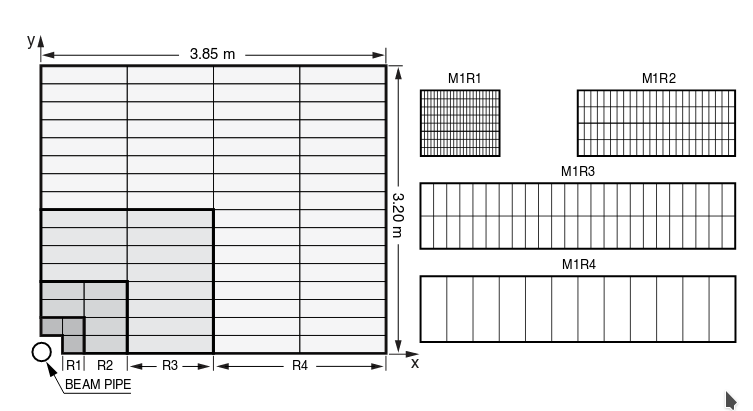
\includegraphics[width = 1.0\textwidth]{figs/trimuon/pad.png}
        \caption{Schematic view of the muon station slicing into x-y pads. This is left quadrant of M1 station, showing decreasing granularity of the muon stations away from the beam. This figure has been taken from \cite{LHCb-DP-2012-002}. M1R1 is the innermost region and M1R4 is the outermost region of the M1 station. }
        \label{fig:pads}
\end{figure}

\subsection{Muon PID variables based on sharing hits \mybox{ULRIK}}
\label{bugs}

Another way of identifying muon tracks is based on variable, \texttt{nShared}, which gives number of tracks with shared hits in the muon stations. For each hit within \gls{FOI} of the extrapolated track, the \texttt{nShared} algorithm will check whether any other track was built using the given hit. In this case, the muon track which has bigger distance between the extrapolation coordinates and the hit coordinates is increased by 1 and the other track becomes the hit owner track. Hence this integer \gls{PID} variable helps supressing \textit{ghost} tracks and \textit{clones} if no tracks have hits in common with the owner of the track (\texttt{nShared==0}).

%\subsection{Different \texttt{nShared} definitions for Run \Rn{1} and Run \Rn{2}}
To make sure that muons for \Bmumumu are not coming from these spurious tracks,  \texttt{nShared==0} for all three muons is required. These three muon tracks will not to share hits in muon stations with any other downstream or long tracks. In analysing data, there were features in the Muon ID alghorithm, software that calculates most of muon \gls{PID} variables, which changed between Run \Rn{1} and Run \Rn{2} and will be discussed in greater detail, as it impacts the selection performed for \Bmumumu search.

The first feature that is different between Run \Rn{1} and Run \Rn{2} arises from the calculation of the distance between the extrapolation and the hit in \texttt{nShared} algorithm.
In \textit{Stripping 21} used for 2012 and \textit{21r1} used for 2011 data, it was discovered that the distance between extrapolated track and hit was wrongly calculated. This mistake was corrected before \textit{Stripping 23}, used for analysing 2015 data. 

Secondly, information from M1 station was used to calculate distances, even though M1 information is not usually used for Muon ID algorithm.  For analysts, this feature was present across all reconstruction software and hence it is consistent within stripping version, meaning that simulation and data is affected in the same way.

In \textit{Stripping 23}, the Muon ID algorithm was rewritten to adapt for parallelisation that needs to be done in order to meet criteria for upgrade of \gls{LHCb}. There were two mistakes introduced prior to 2015 data taking.
Firstly, an array was defined with 4-elements $[0,3]$ to store information about $x$ and $y$ coordinates of the hits. However, an iteration occurred by filling $[1,4]$ array (M2-M5 station) resulting in 5-element array where 0-th element was not filled. Despite this, it turns out to be well-behaved and has no impact on physics.

Further in the process, however, this information is used to calculate the sum and average of distances per station between the hits and extrapolations. This algorithm again iterates over $[0,3]$ arrays, meaning that no information is used from M5 muon station. This obviously has effect, but again it is consistent across the reconstruction version.

%\newline Summary of these features can be found in \href{https://indico.cern.ch/event/612764/contributions/2567244/attachments/1449649/2234804/20170426\_nShared.pdf}{\color{blue} in this presentation} 
The interplay between all discussed features for \bjpsimumuk can be seen in Figure~\ref{fig:nSharedvar}, which see shift in distribution of \texttt{nShared} for 2016 data taking, making the muons less isolated.

\begin{figure}[h!]
\centering
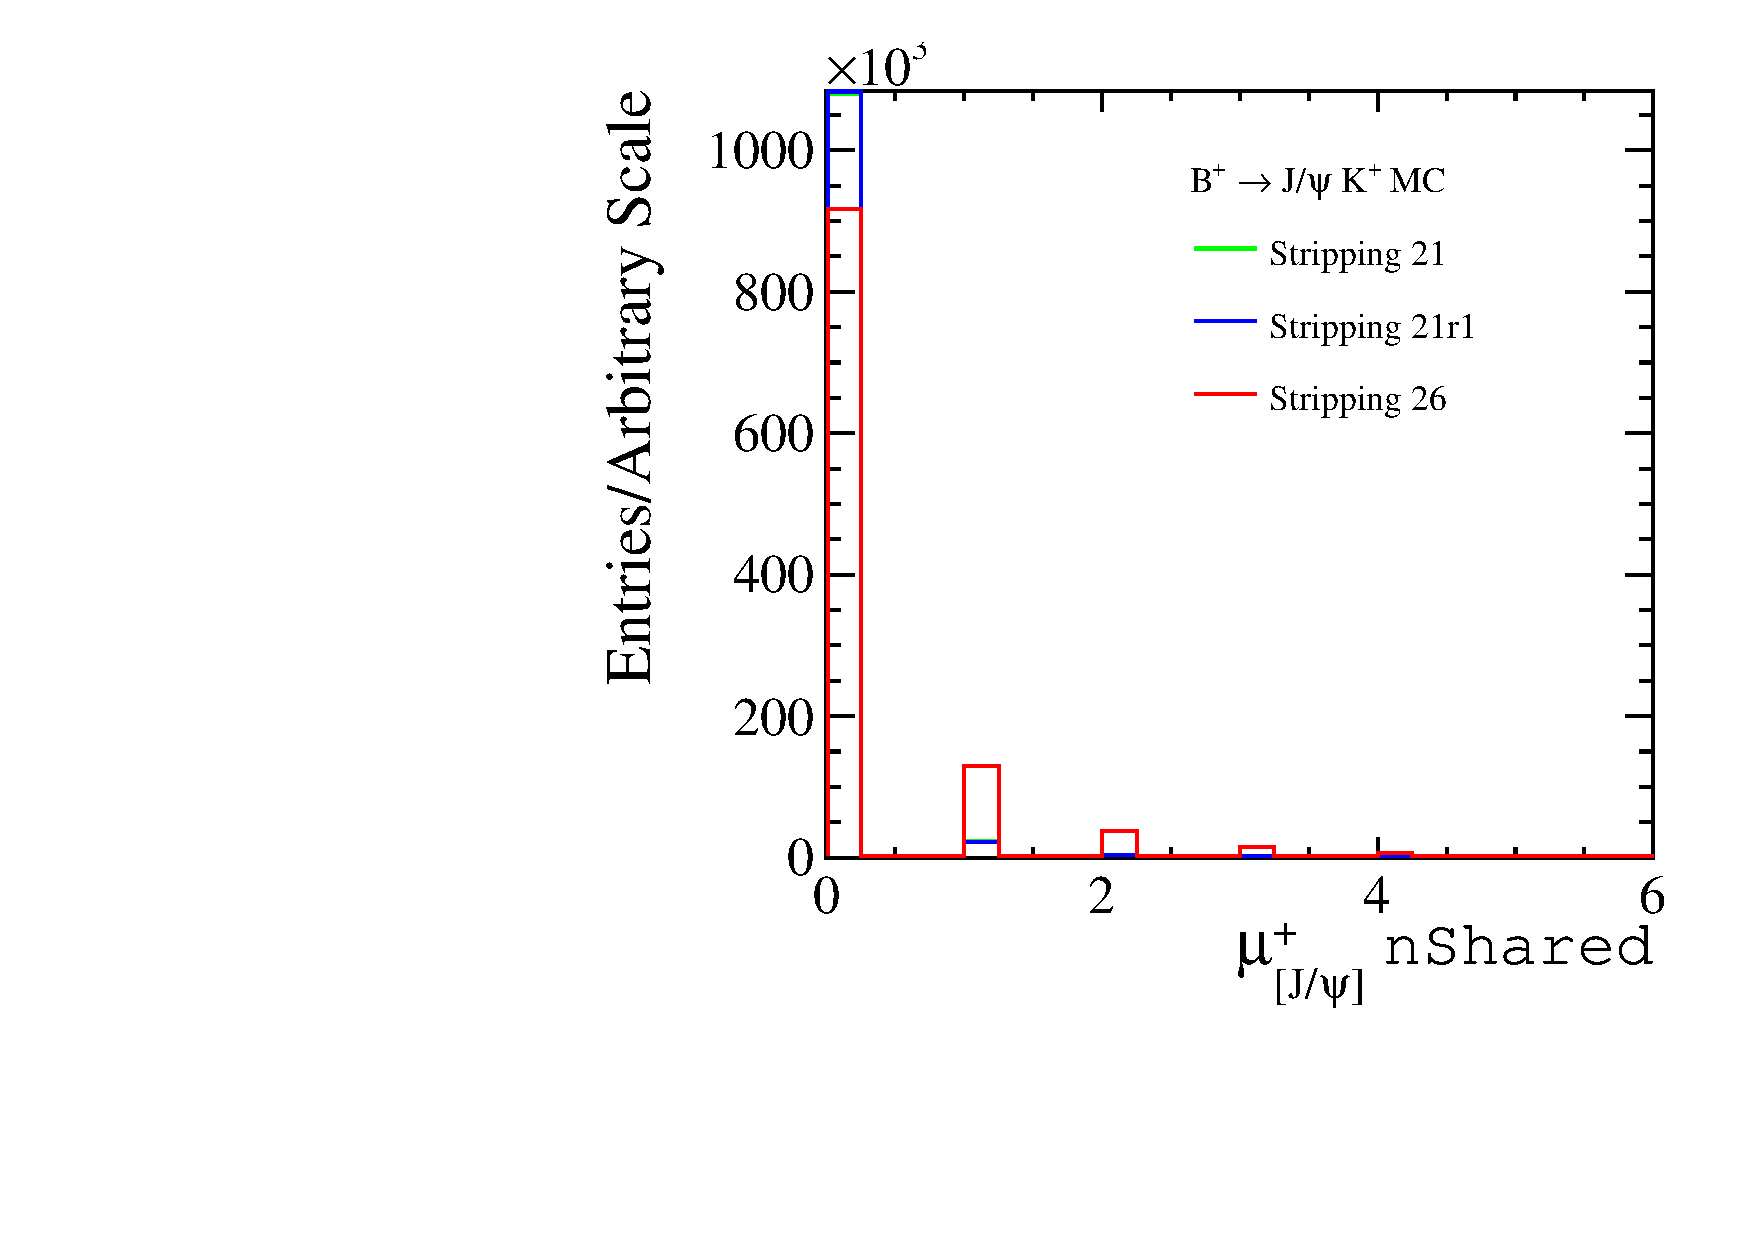
\includegraphics[width=0.5\linewidth]{trimuon/plotvariablemu1_nSharedJPSIKMC.pdf}\put(-40,133){(a)}
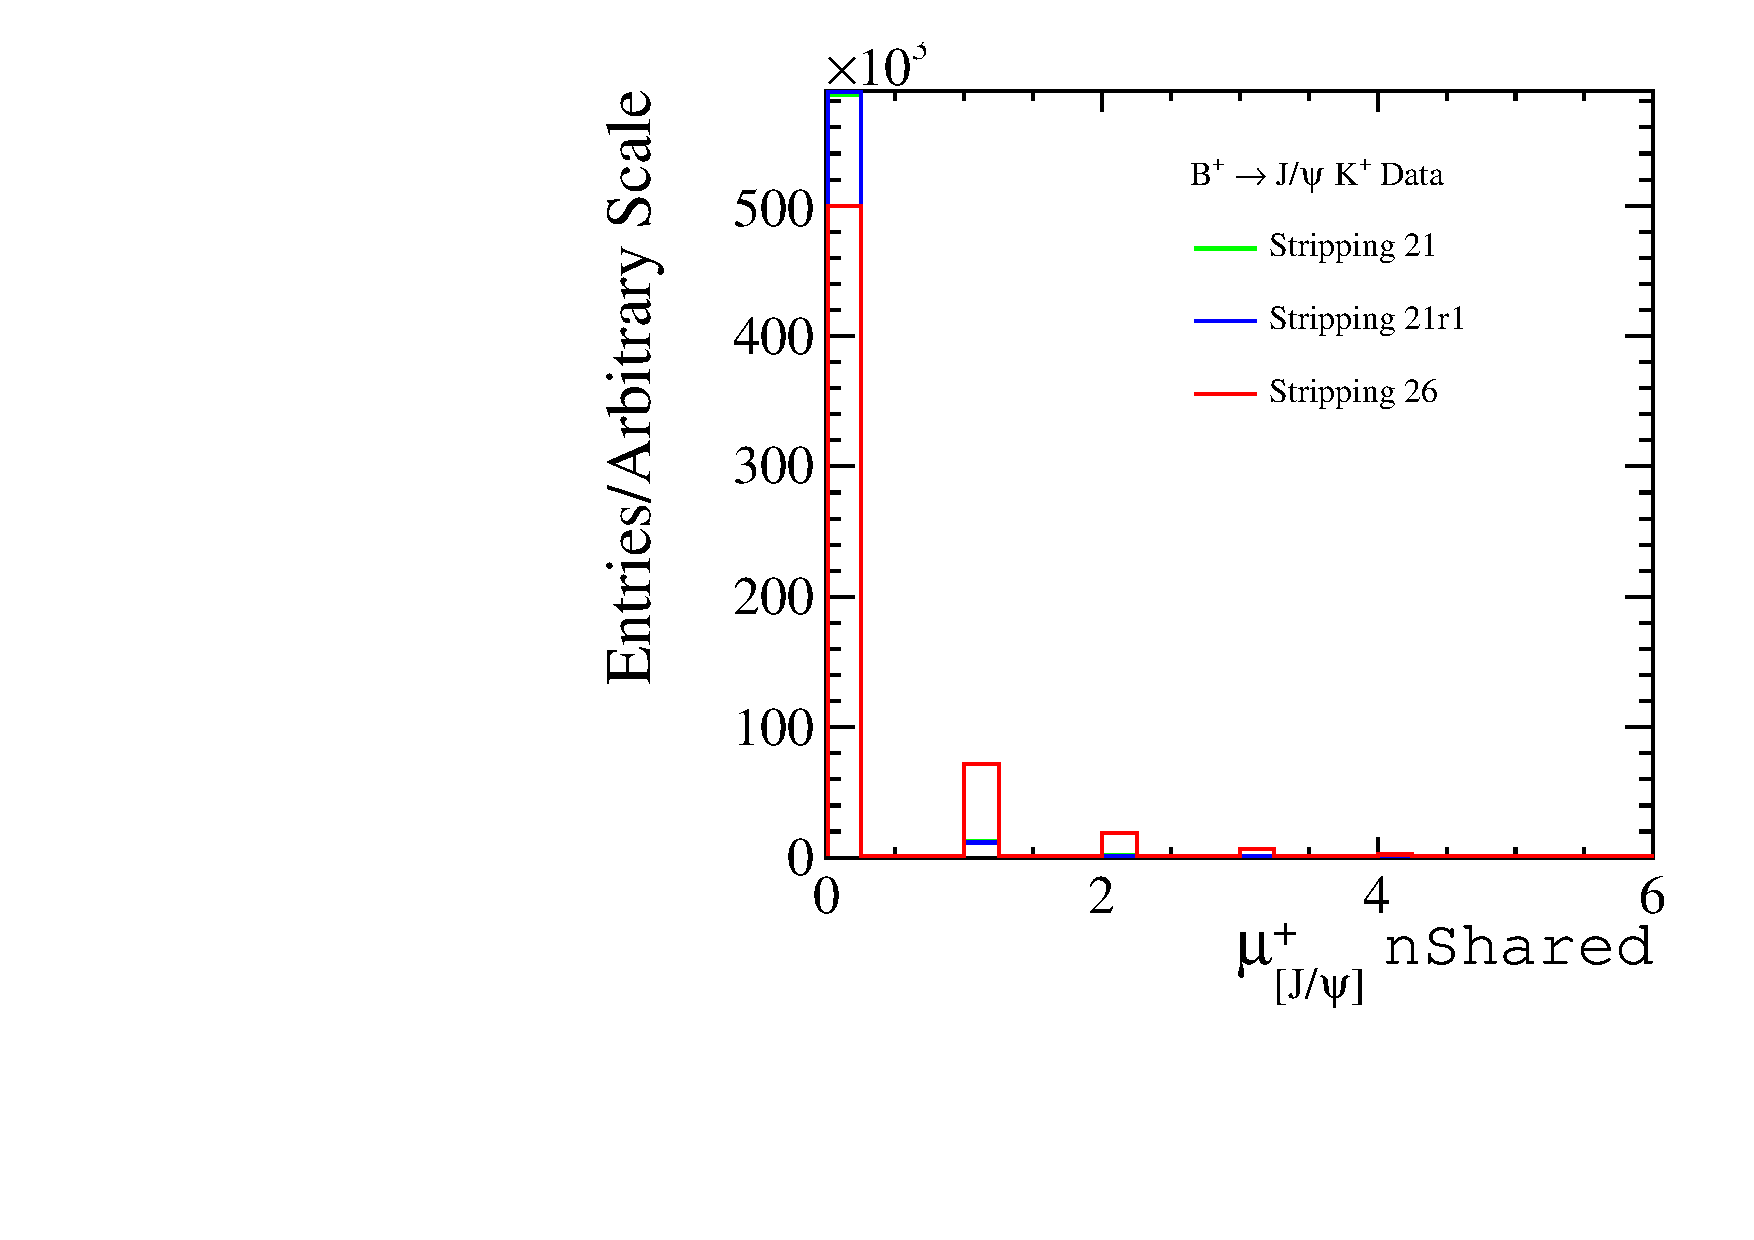
\includegraphics[width=0.5\linewidth]{trimuon/plotvariablemu1_nSharedJPSIKDATA.pdf}\put(-40,133){(b)}
	\caption{ (a) The \texttt{nShared} variable in simulation, (b) data for \bjpsimumuk in different stripping versions corresponding to 2012 (\textit{Stripping 21}), 2011 (\textit{Stripping 21r1}), 2016 (\textit{Stripping 26}) data-taking. There is shift of distribution in \textit{Stripping 26} towards less isolated tracks.}
\label{fig:nSharedvar}
%\vspace*{-1.0cm}
\end{figure}


This will have inevitably and impact on the \gls{PID} probabilities. Using the same calibration channels as in \autoref{muonperf}, misID and ID rates can be seen in Figure~\ref{fig:nSharedRun1andRun2}. As the tracks tend to be less isolated in \textit{Stripping 26}, typical of non-signal like events, the misID rate is expected to be higher for the same working point (ID efficiency).

\begin{figure}[h!]
\centering
%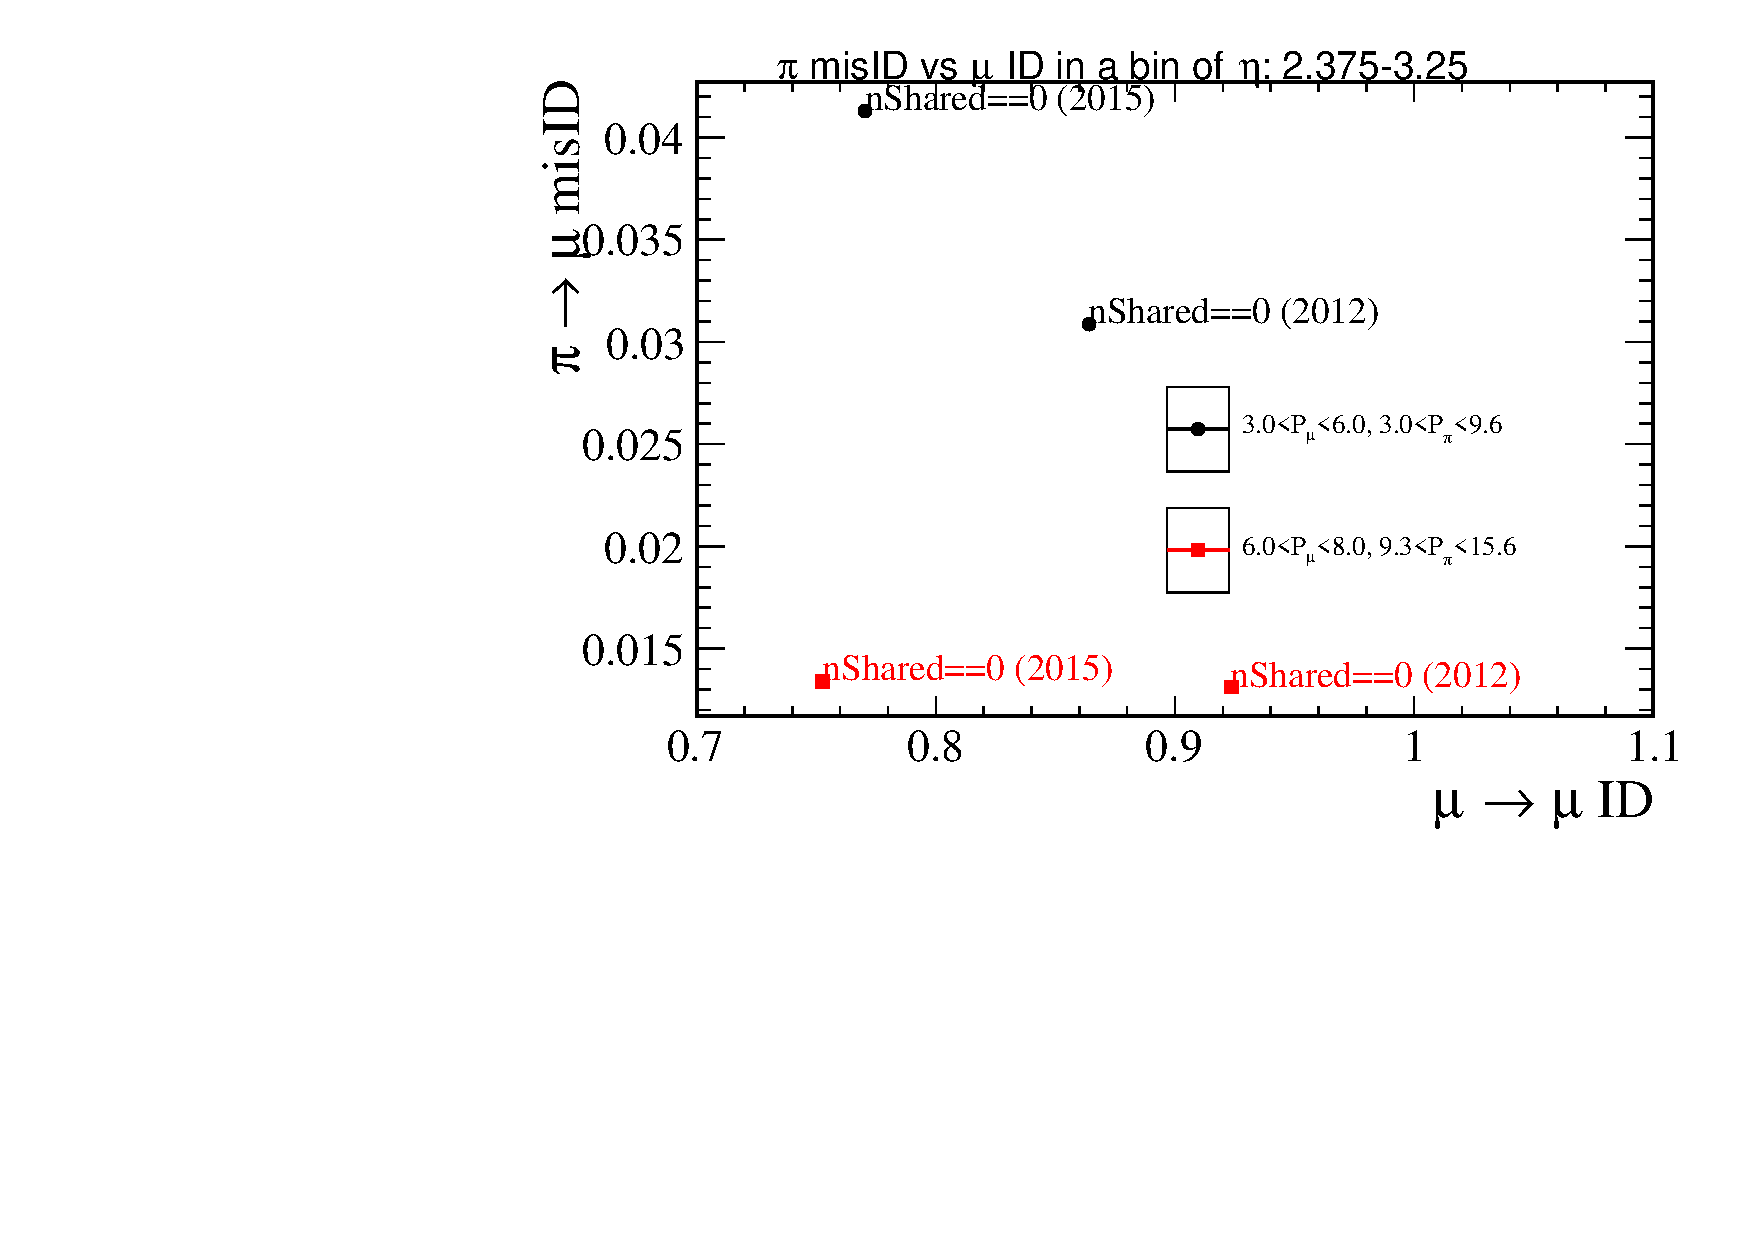
\includegraphics[width=0.52\linewidth]{compareRun1and2016selection/final_comparedirectly2012vs2015_nolog.pdf}%
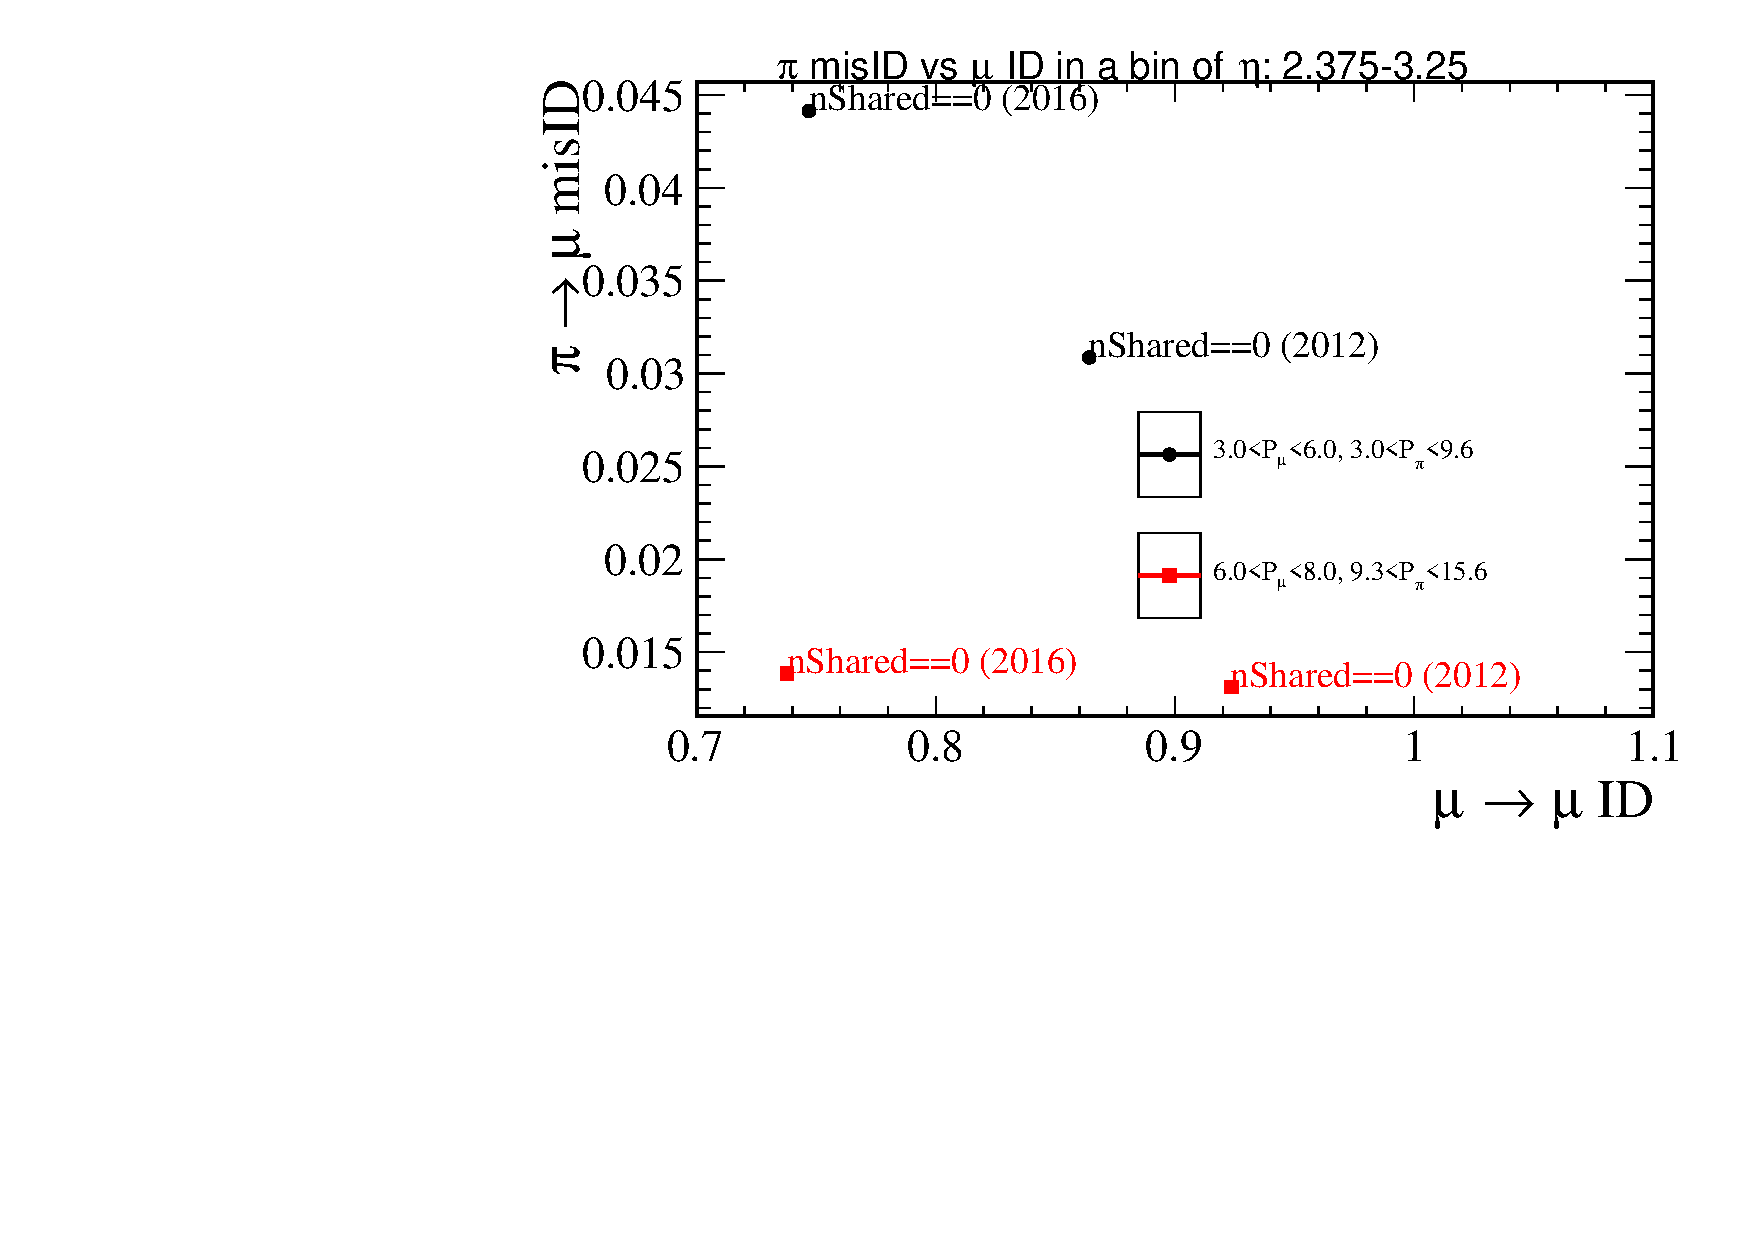
\includegraphics[width=0.7\linewidth]{trimuon/final_comparedirectly2012vs2016_nolog.pdf}
	\caption{ID and misID probabilities from standard calibration datasets from 2012 (\textit{Stripping 21}) 2016 (\textit{Stripping 26}), binned using default 2-dimensional binning scheme in momentum $p$ and pseudorapidity $\eta$. In this plot, ID and misID rate in central bin of $\eta$ and first and second bin in $p$ are compared. This demonstrates that for same ID efficiency, the misID rate is significantly higher in 2016.}
\label{fig:nSharedRun1andRun2}
%\vspace*{-1.0cm}
\end{figure}

\subsection{Muon PID variables based on regression techniques \mybox{ULRIK}}
Similar to the \texttt{DLLmu} variable in \autoref{muonID}, which combines all the information from the detector into a global likelihood, it is possible to feed all the different variables to a neural network, which can then produce an output corresponding to the probability of a particle to be of a certain species. \texttt{Probnn${x}$}, where $x$ is the species of interest, is calculated and can be used also for muon identification. Compared to $DLL{x}$ variables, \texttt{Probnn${x}$} variables tend to have smaller correlation with the kinematics of the particle, and hence are more useful with decays where particles are soft, such as \Bmumumu. As with any machine learning algorithms, the selection of the training sample is important as well as input variables. In Run \Rn{1} there were two tunings (trainings) introduced \texttt{V2} and \texttt{V3}, with more input variables in \texttt{V2}. Depending on the species of particles, \texttt{V2} or \texttt{V3} performed better. In the analysis of \Bmumumu \texttt{Probnn${x}\_$V2} is used.


\section{Clones \mybox{ULRIK}}
When analysing decays with two muons of the same charge, \gls{LHCb} magnet bends these two muons in two separate planes. With two muons of the same sign, it is more likely that their two tracks will be collimated. This poses more difficult task for tracking as it distinguishes these two tracks less well. It is even possible that these two same sign muon tracks are not genuine tracks, but rather subtracks or a copy of another track, \textit{clone tracks}. Two tracks are clones if they share at least 70\% of the hits in the \gls{VELO} and at least 70\% of the hits in the other T-stations. Of course, once it is established that two tracks share this percentage of hits, it has to be established which track is the clone track. This decision is based on the total number of hits and the \gls{trackchi2ndof} comparison of the two tracks.   


\begin{figure}[h!]
\centering
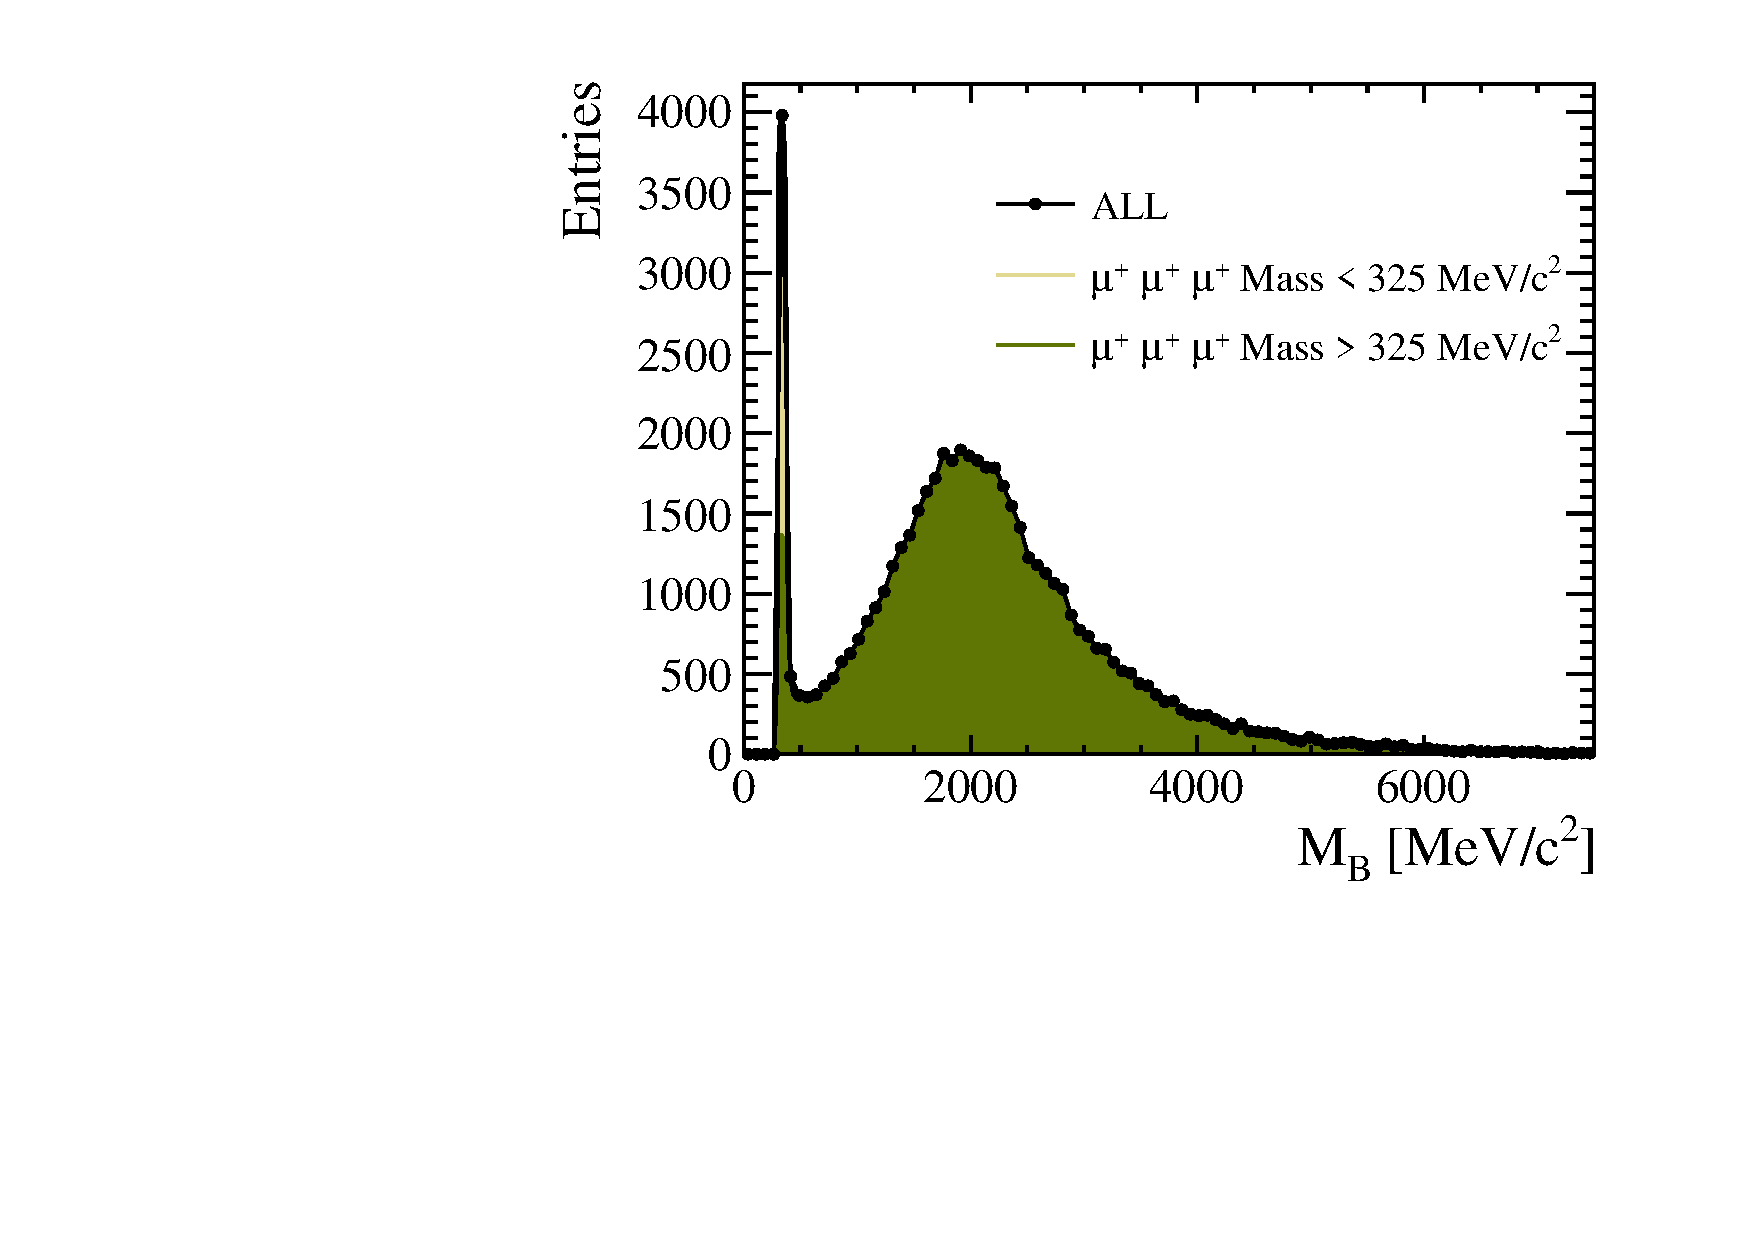
\includegraphics[width=0.5\linewidth]{trimuon/compnice_even_nicer_ONLY_STACKED_HIST_VisibleCorrM.pdf}\put(-50,133){(a)}
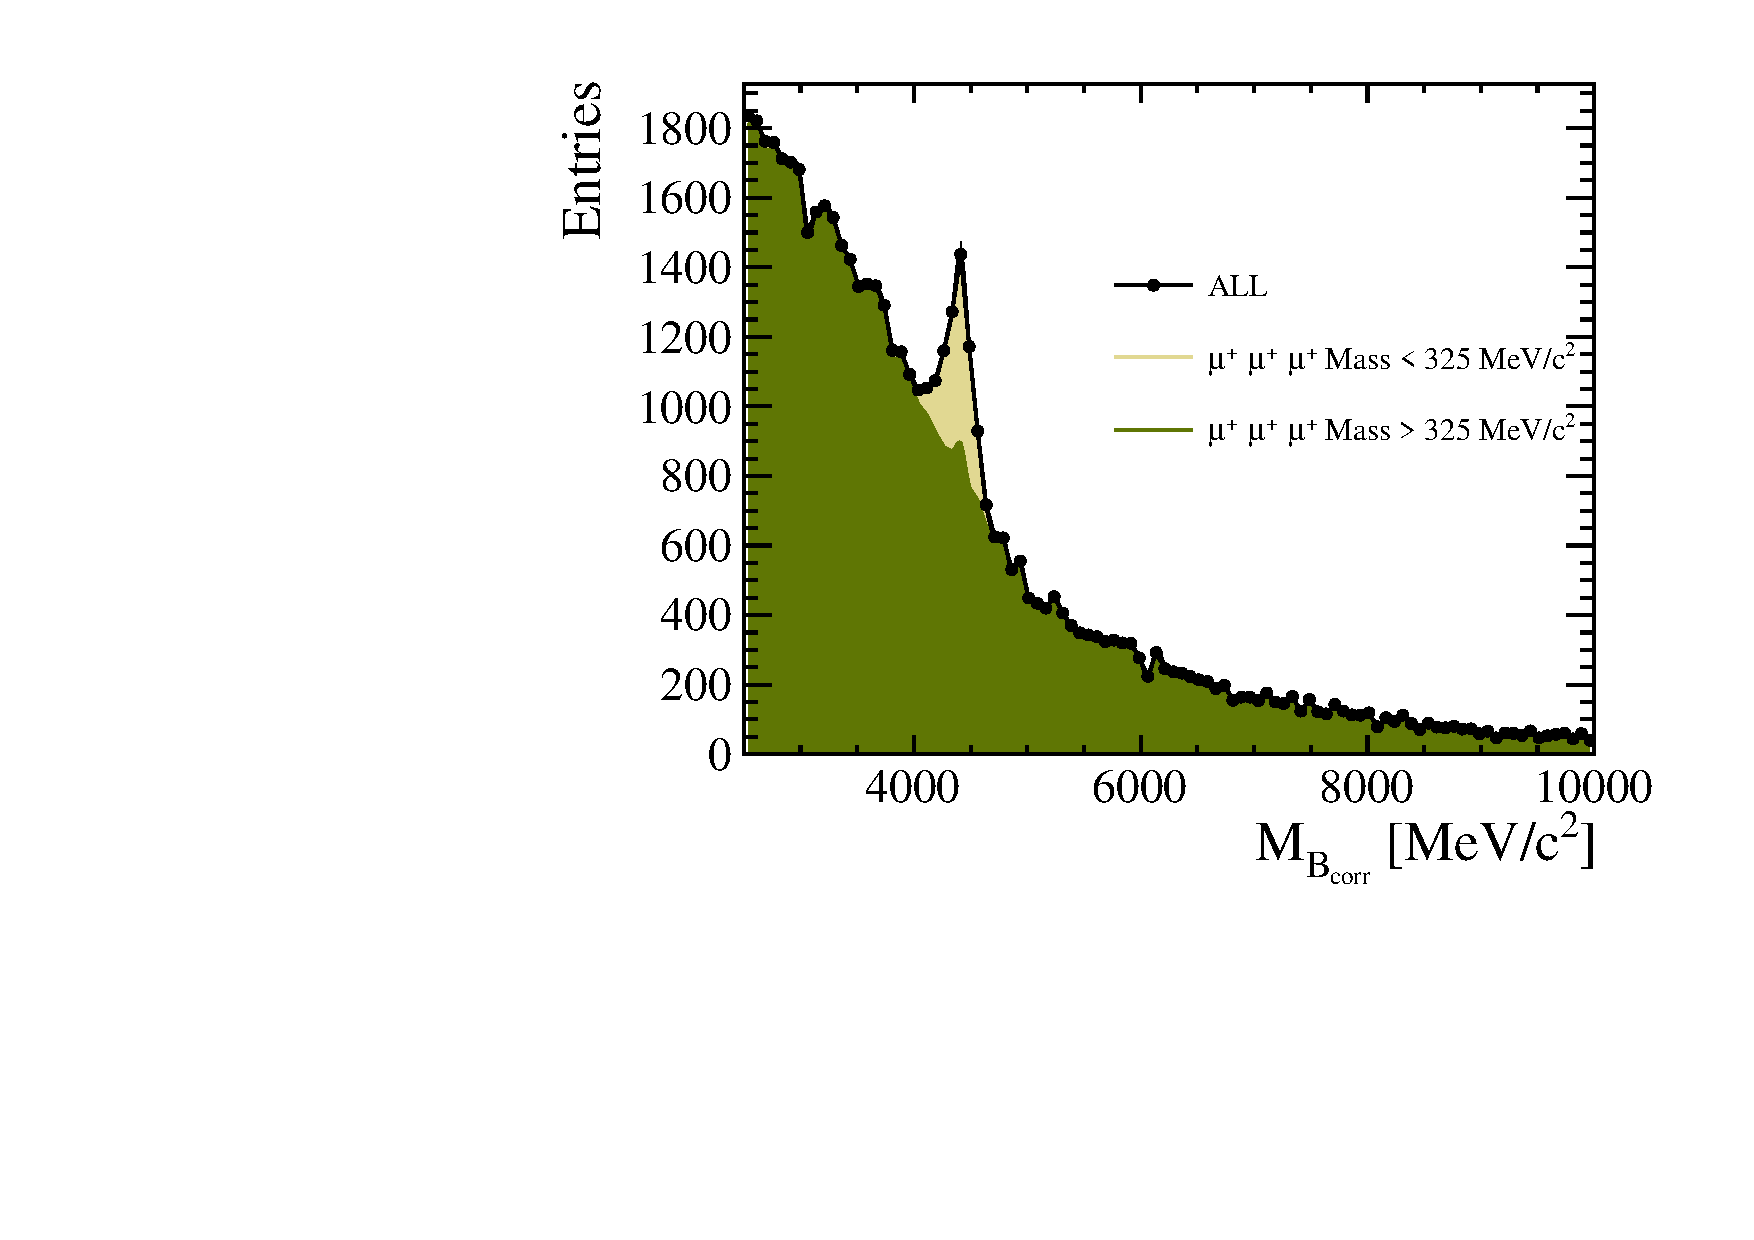
\includegraphics[width=0.5\linewidth]{trimuon/compnice_even_nicer_ONLY_STACKED_HIST_CorrM.pdf}\put(-50,133){(b)}
	\caption{(a) Visible and (b) corrected mass of $B$, shows a clear peak coming from clones in 2012 same sign data sample. }
\label{fig:Clones}
%\vspace*{-1.0cm}
\end{figure}


In search for \Bmumumu two muons have the same charge, and hence are affected by the \textit{clones}, which needs to be understood. In this case, sample with three muons of same sign was obtained, where the effect is even more prominent and can create potentially \textit{fake peaks} in visible mass spectrum. \textit{Clones} peak at well defined visible mass 
\begin{equation}
	M_{B}=\sqrt{(3 \times M_{\mu})^{2}}\approx 318 \mevcc
	\label{eq:invmass}
\end{equation}

Once translated into corrected mass, these \textit{fake peaks} are smeared and look like genuine resonances with resolution as seen in \autoref{fig:Clones}.  


The shape of genuine resonance comes as a result of \gls{LHCb} many factors: vertexing, tracking and trigger selection. As there are three parallel tracks, the vertex of the system is not well defined. However, the vertex fitting of the \gls{PV} and \gls{SV} is functional and \gls{vertexchi2ndof} is good as these tracks are subtracks of each other.  \textit{Clones} can be, however, differentiated by the position of the decay vertex of $B$, \autoref{fig:ClonesFD} as well as the occupancy in the tracking, \gls{OT} as seen in \autoref{fig:ClonesOT}.

\begin{figure}[h!]
\centering
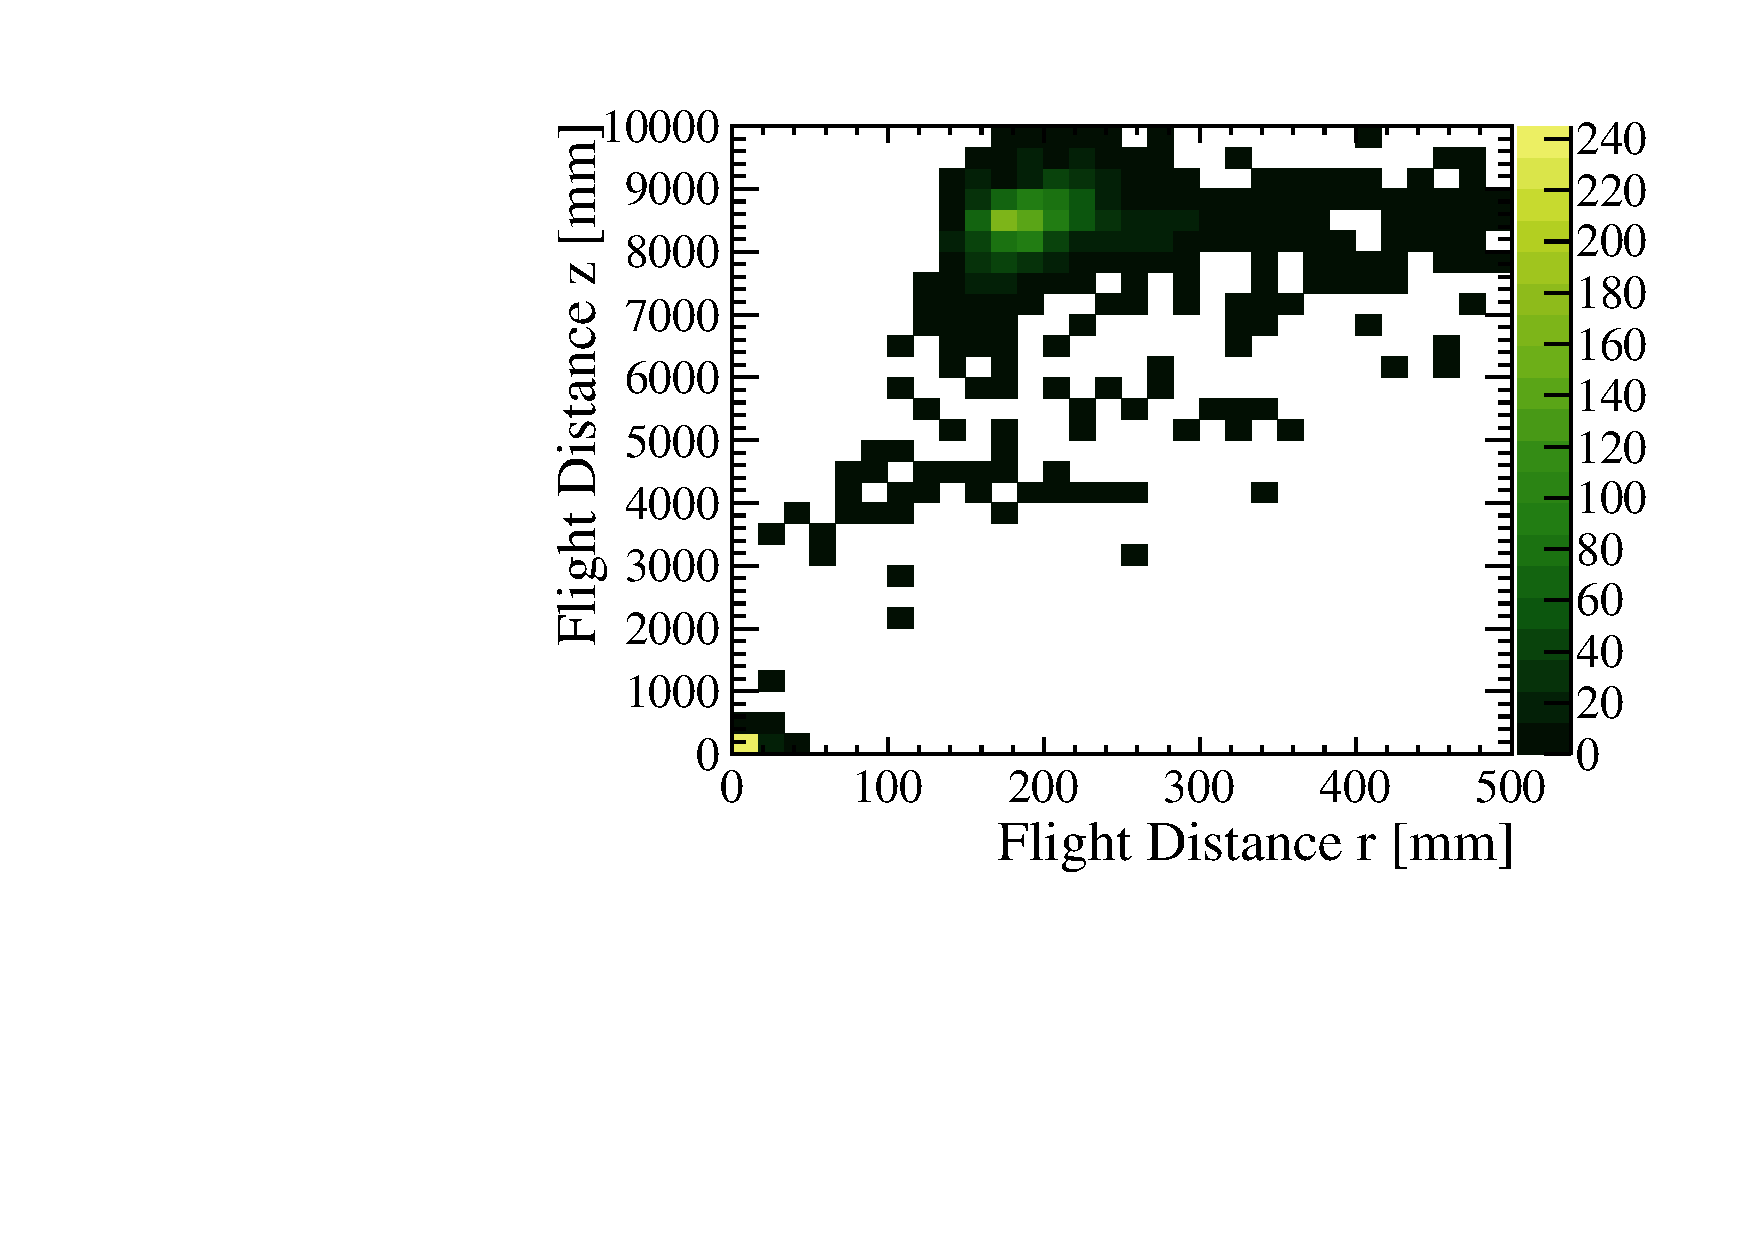
\includegraphics[width=0.5\linewidth]{trimuon/VertexInfoClone.pdf}\put(-50,133){(a)}
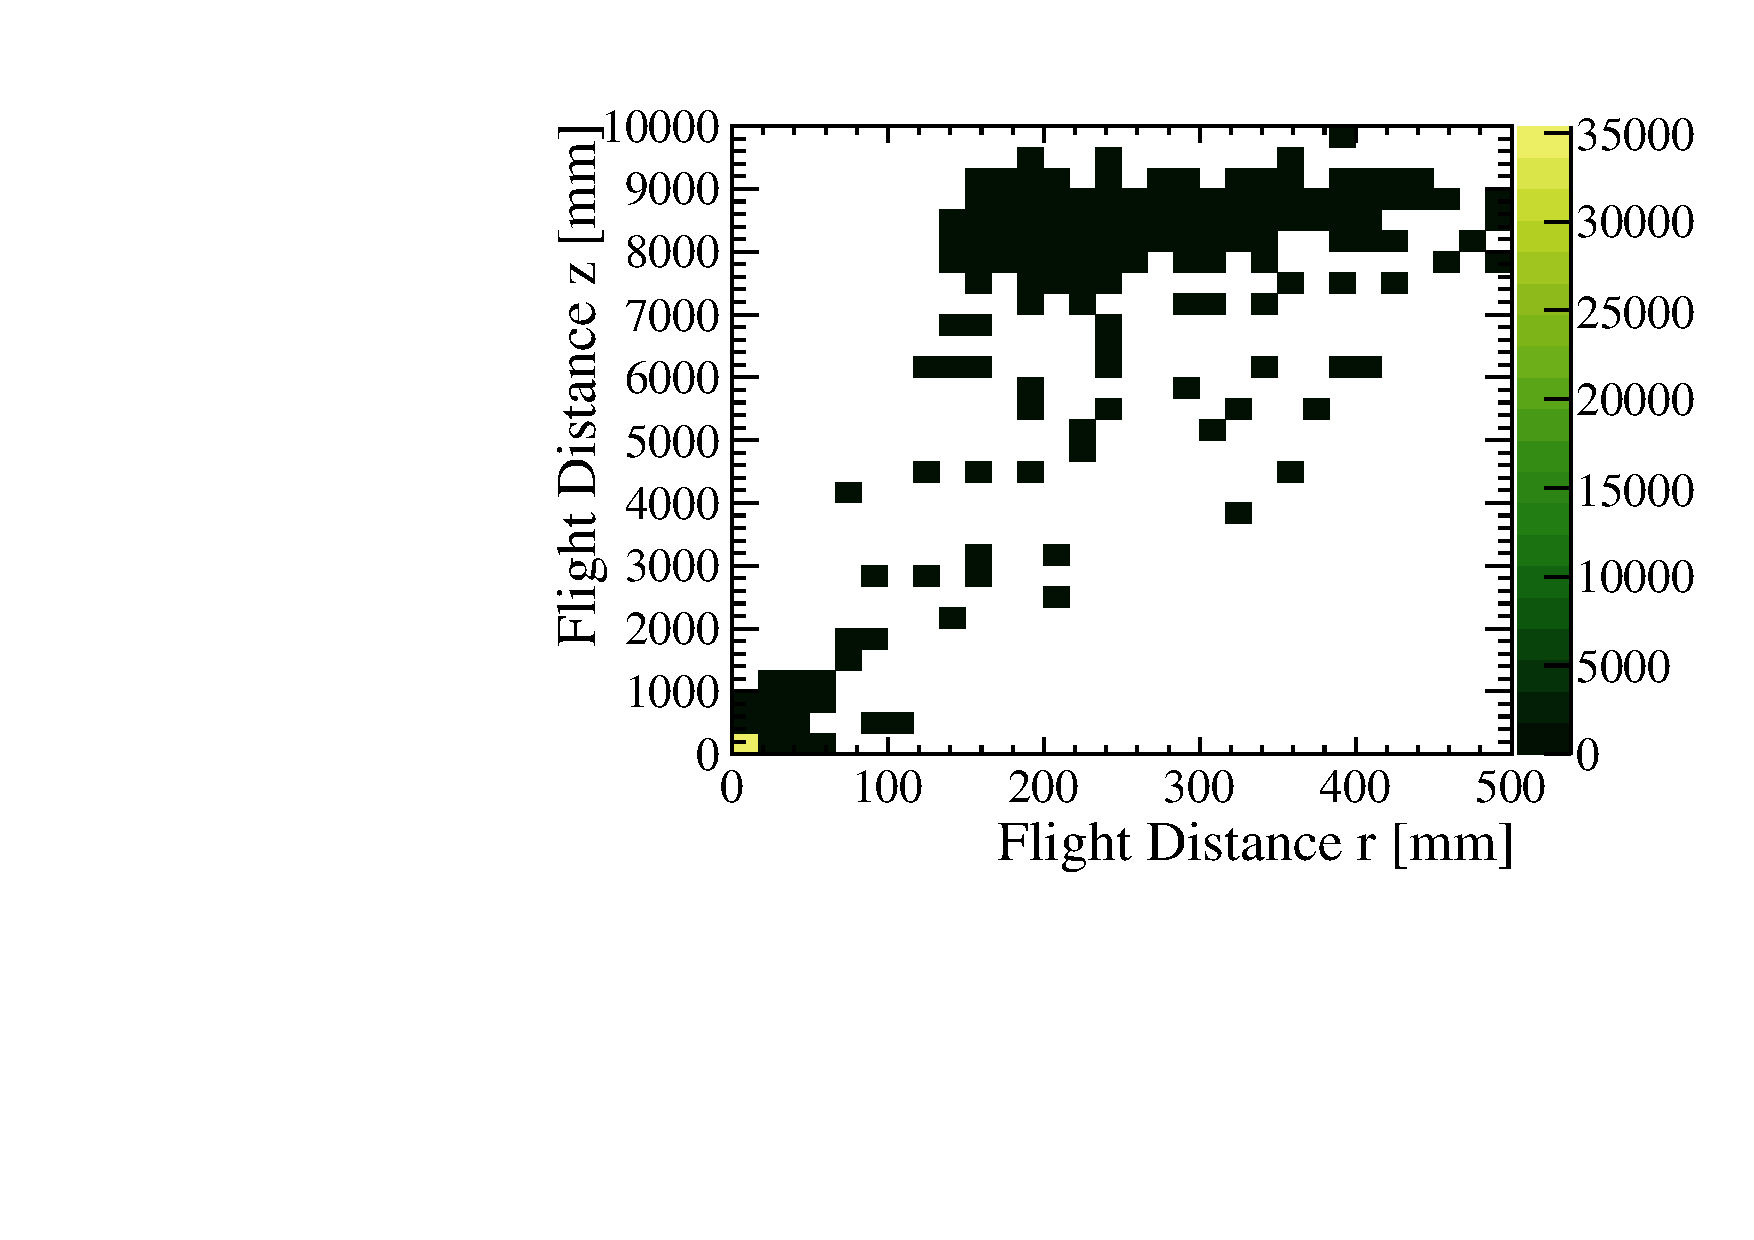
\includegraphics[width=0.5\linewidth]{trimuon/VertexInfoNoClone.pdf}\put(-50,133){(b)}
	\caption{(a) Clone and (b) no clones flight distance properties. It can be seen that \textit{clone} tracks have their decay vertex placed at the end of the detector, whereas regular good tracks will decay within \gls{VELO}.}
\label{fig:ClonesFD}
%\vspace*{-1.0cm}
\end{figure}


\begin{figure}[h!]
\centering
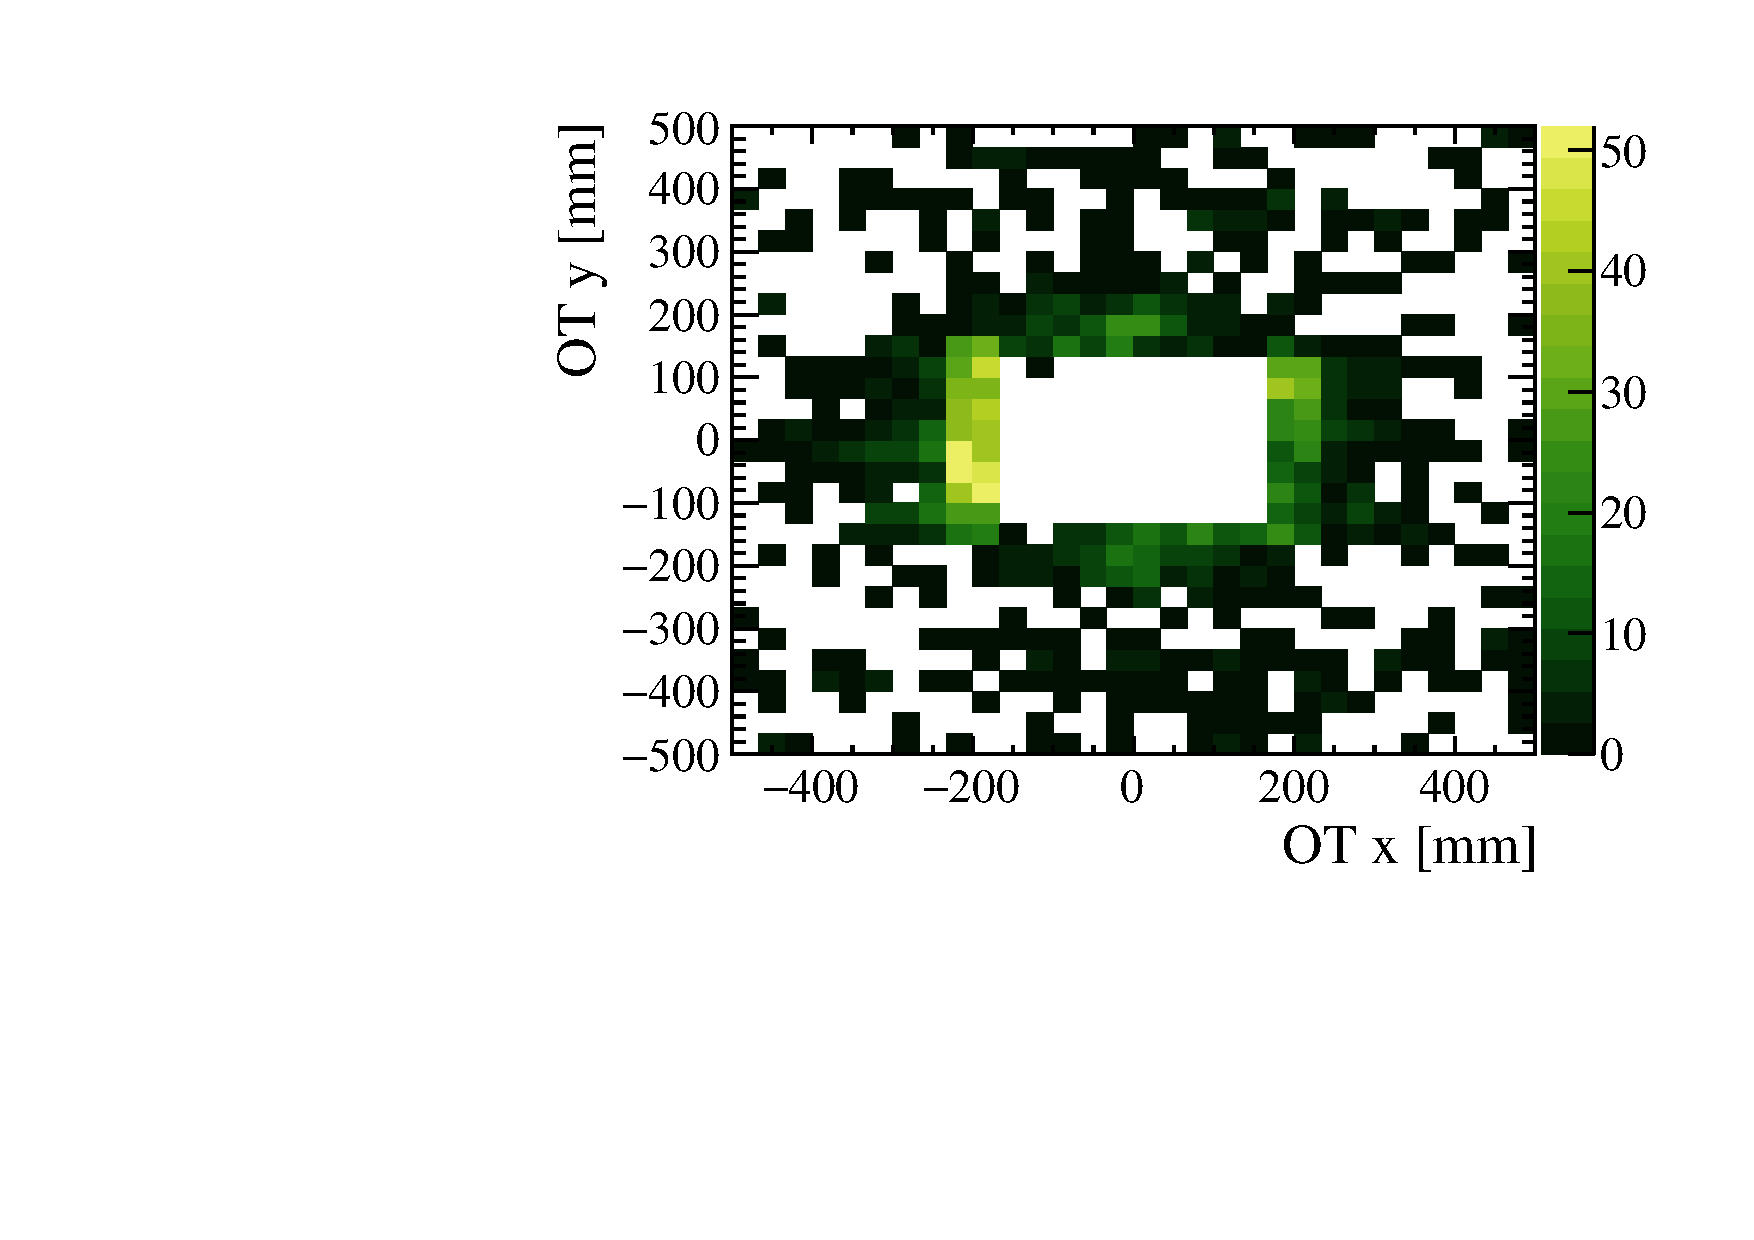
\includegraphics[width=0.5\linewidth]{trimuon/OTxandyClone.pdf}\put(-50,133){(a)}
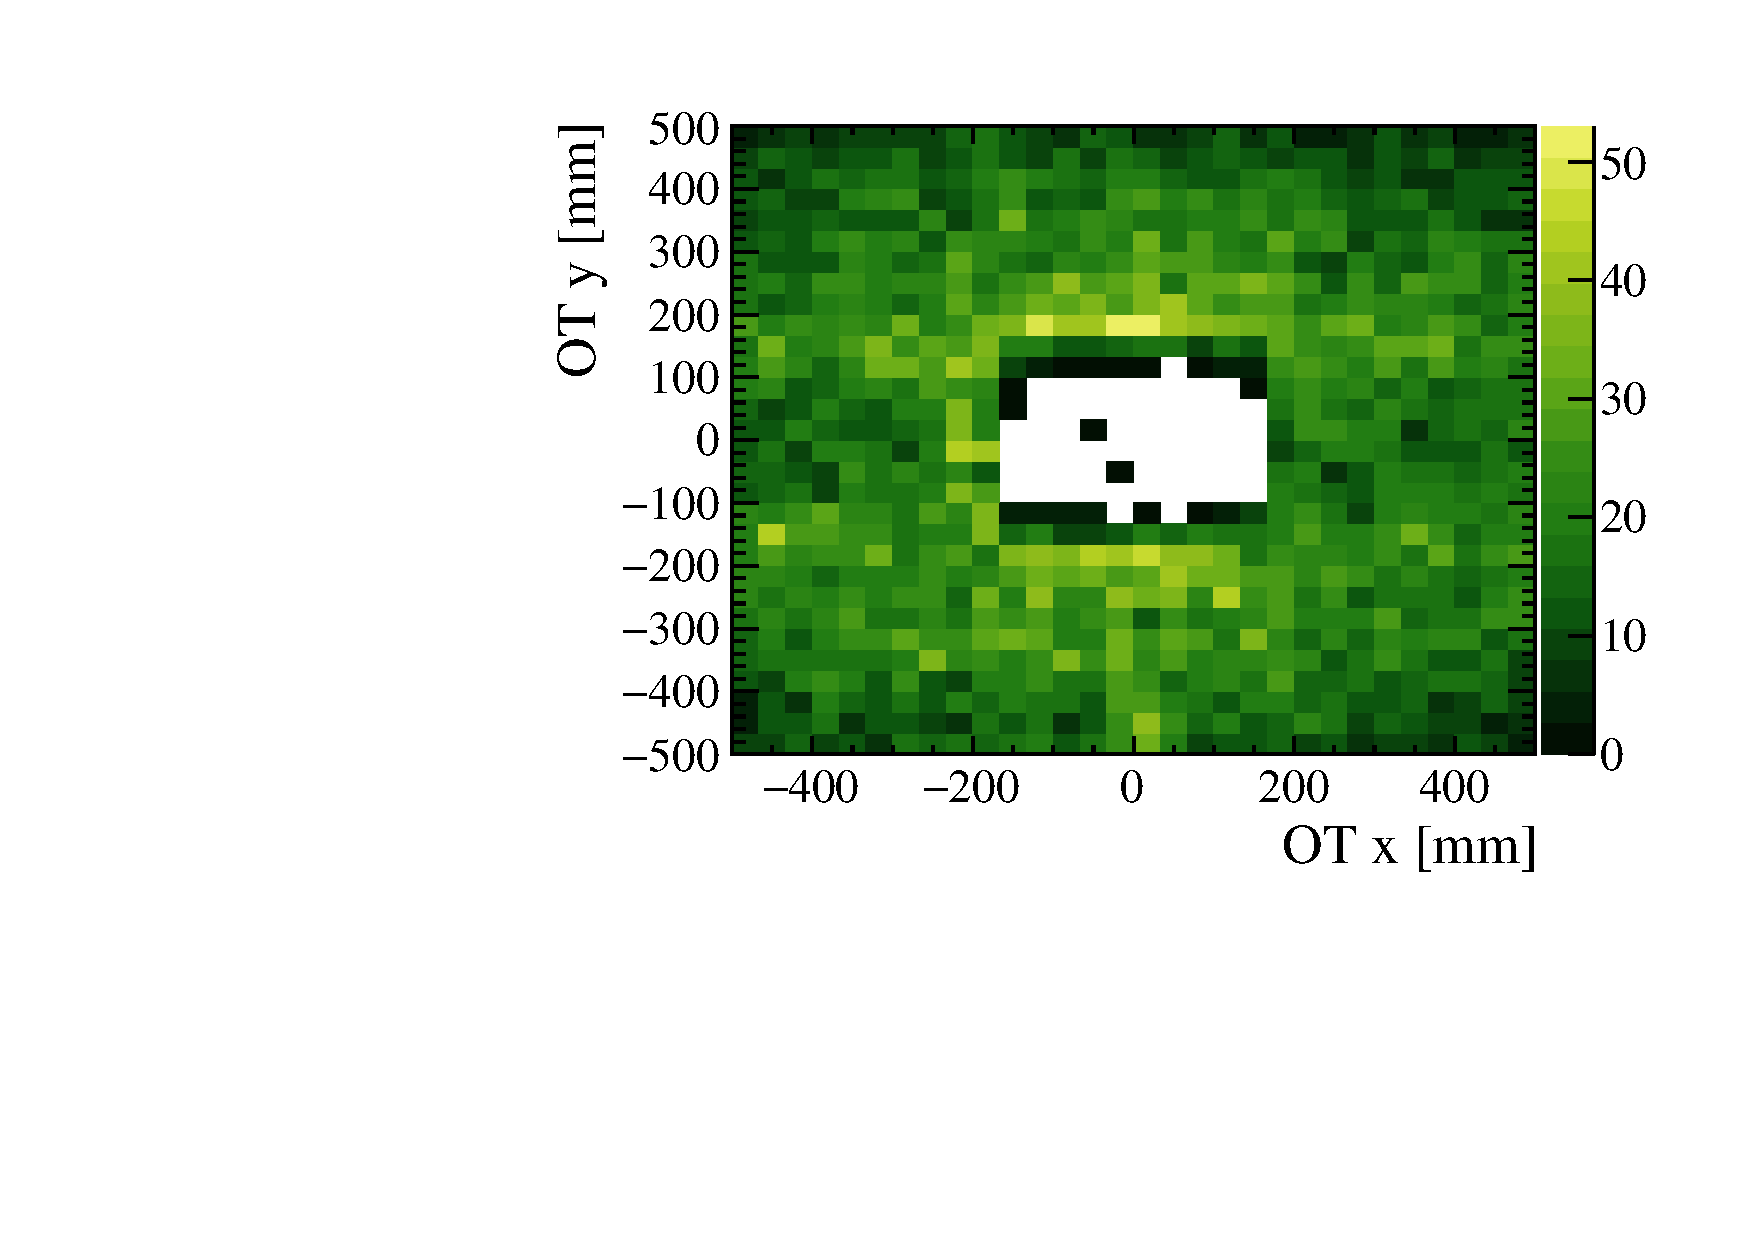
\includegraphics[width=0.5\linewidth]{trimuon/OTxandyNoClone.pdf}\put(-50,133){(b)}
	\caption{The occupancy difference in the \gls{OT} detector between (a) clones and (b) real tracks in the \Gls{OT} at the distance 9450 \mm along the \gls{LHCb}. \textit{Clones} are concentrated along the inner edge of the \gls{OT}. Good muon tracks will cover most of \gls{OT} evenly.}
\label{fig:ClonesOT}
%\vspace*{-1.0cm}
\end{figure}

With this typical path for the clones there is a fixed angle of the clones trough the detector (the angle between muon momentum the z-axis), which is calculated using information from \gls{OT} in a following way:

\begin{equation}
	\arctan(\theta)=\arctan\Big(\frac{\gls{FD}\ radius}{\gls{FD}\ distance\ along\ z}\Big)=\arctan\Big(\frac{200\ \mm\ (\autoref{fig:ClonesOT})}{8500\ \mm}\Big) = 0.023 rad. 
\end{equation}


With the \texttt{L0Muon} $p_{T}$ threshold of 1.76 \gevc for 2012 \cite{Albrecht:2013fba}, the typical momentum from about 75  to 120 \gevc is yielded because

\begin{equation}
	p=1.76\gevc/\sin\bigg(\arctan(\theta)=\arctan\Big(\frac{200\ \mm}{8500\ \mm}\Big)\bigg).
\end{equation}

The angle between $B$ flight and trimuon momentum vector, \gls{DIRA}, will also be fixed and have typical value of 0.7 \mrad as seen in \autoref{fig:ClonesDIRA}.

\begin{figure}[h!]
\centering
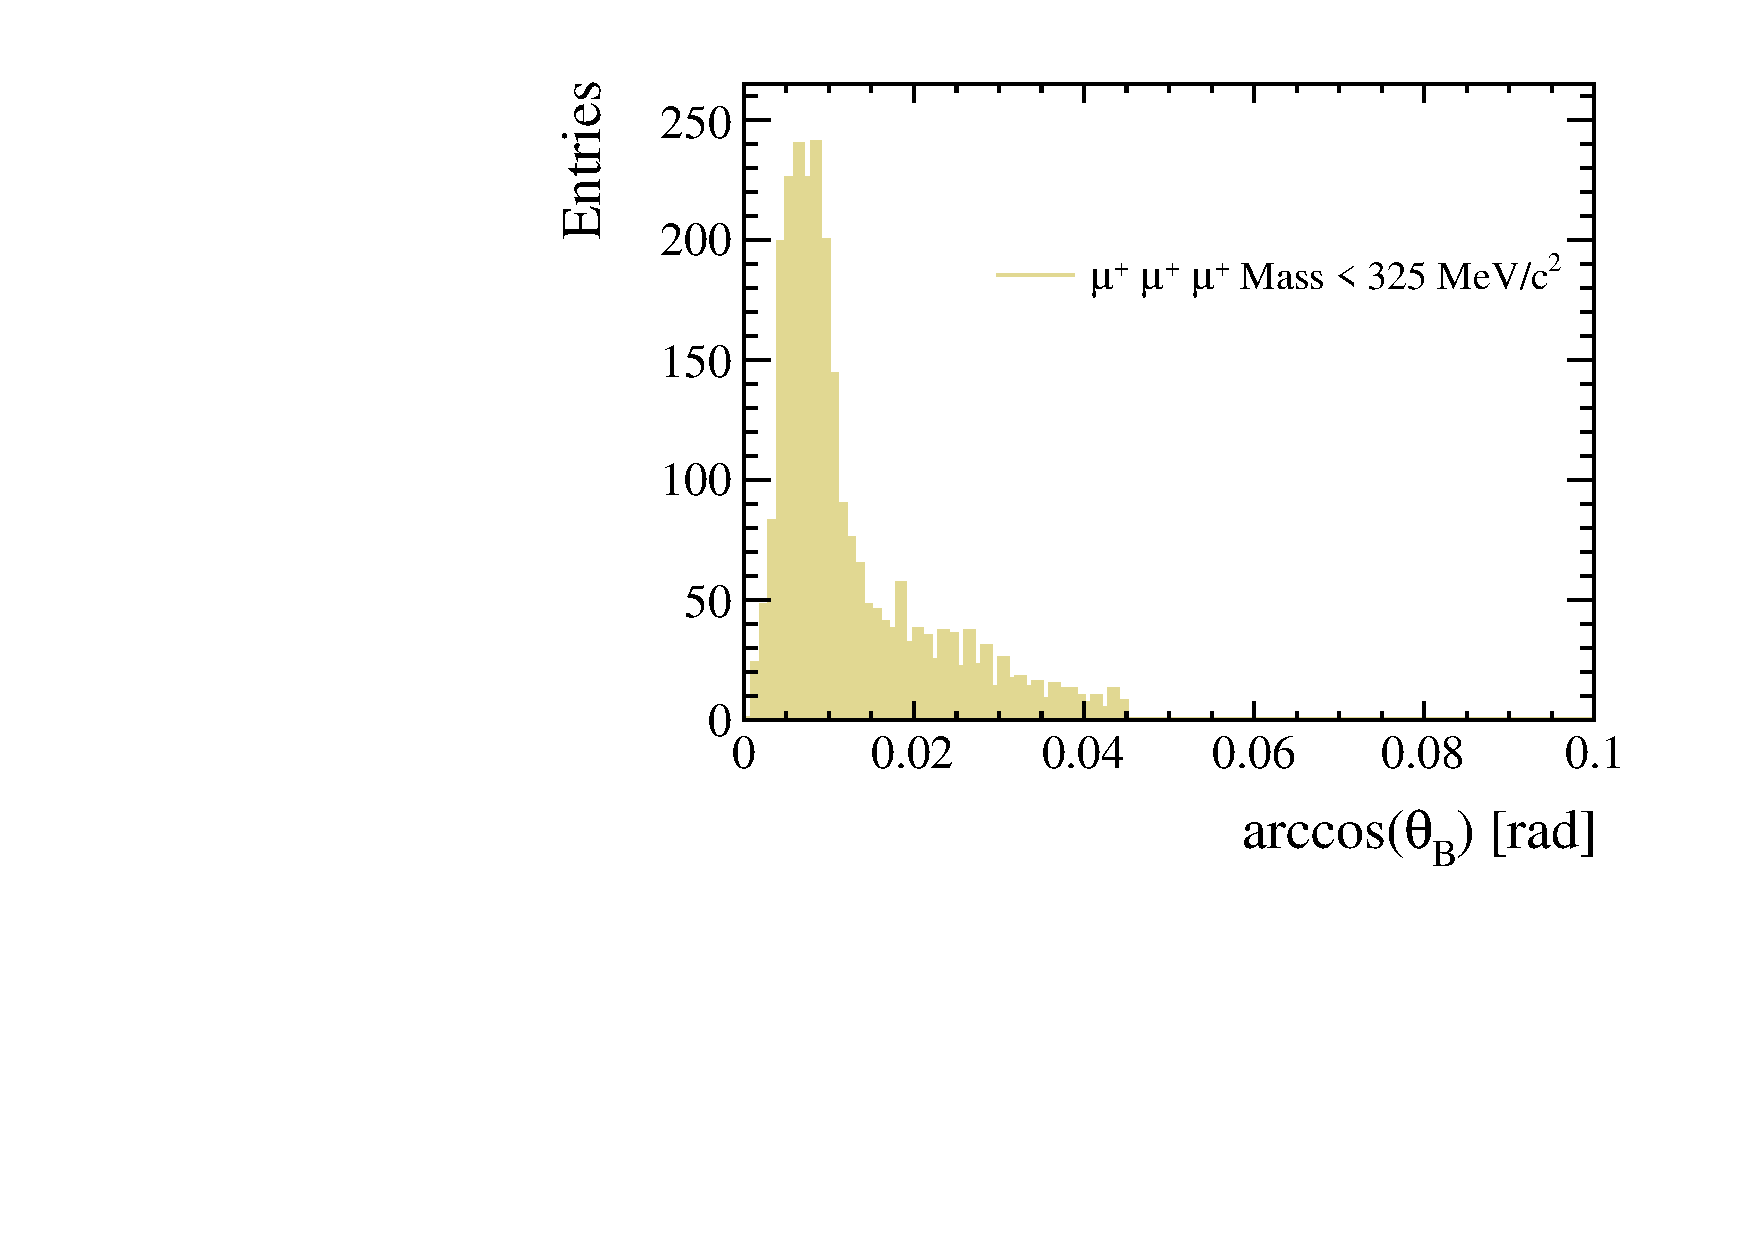
\includegraphics[width=0.5\linewidth]{trimuon/compnice_even_nicer_ONLY_STACKED_HIST_oneFILE_BplusDiraclone.pdf}\put(-50,133){(a)}
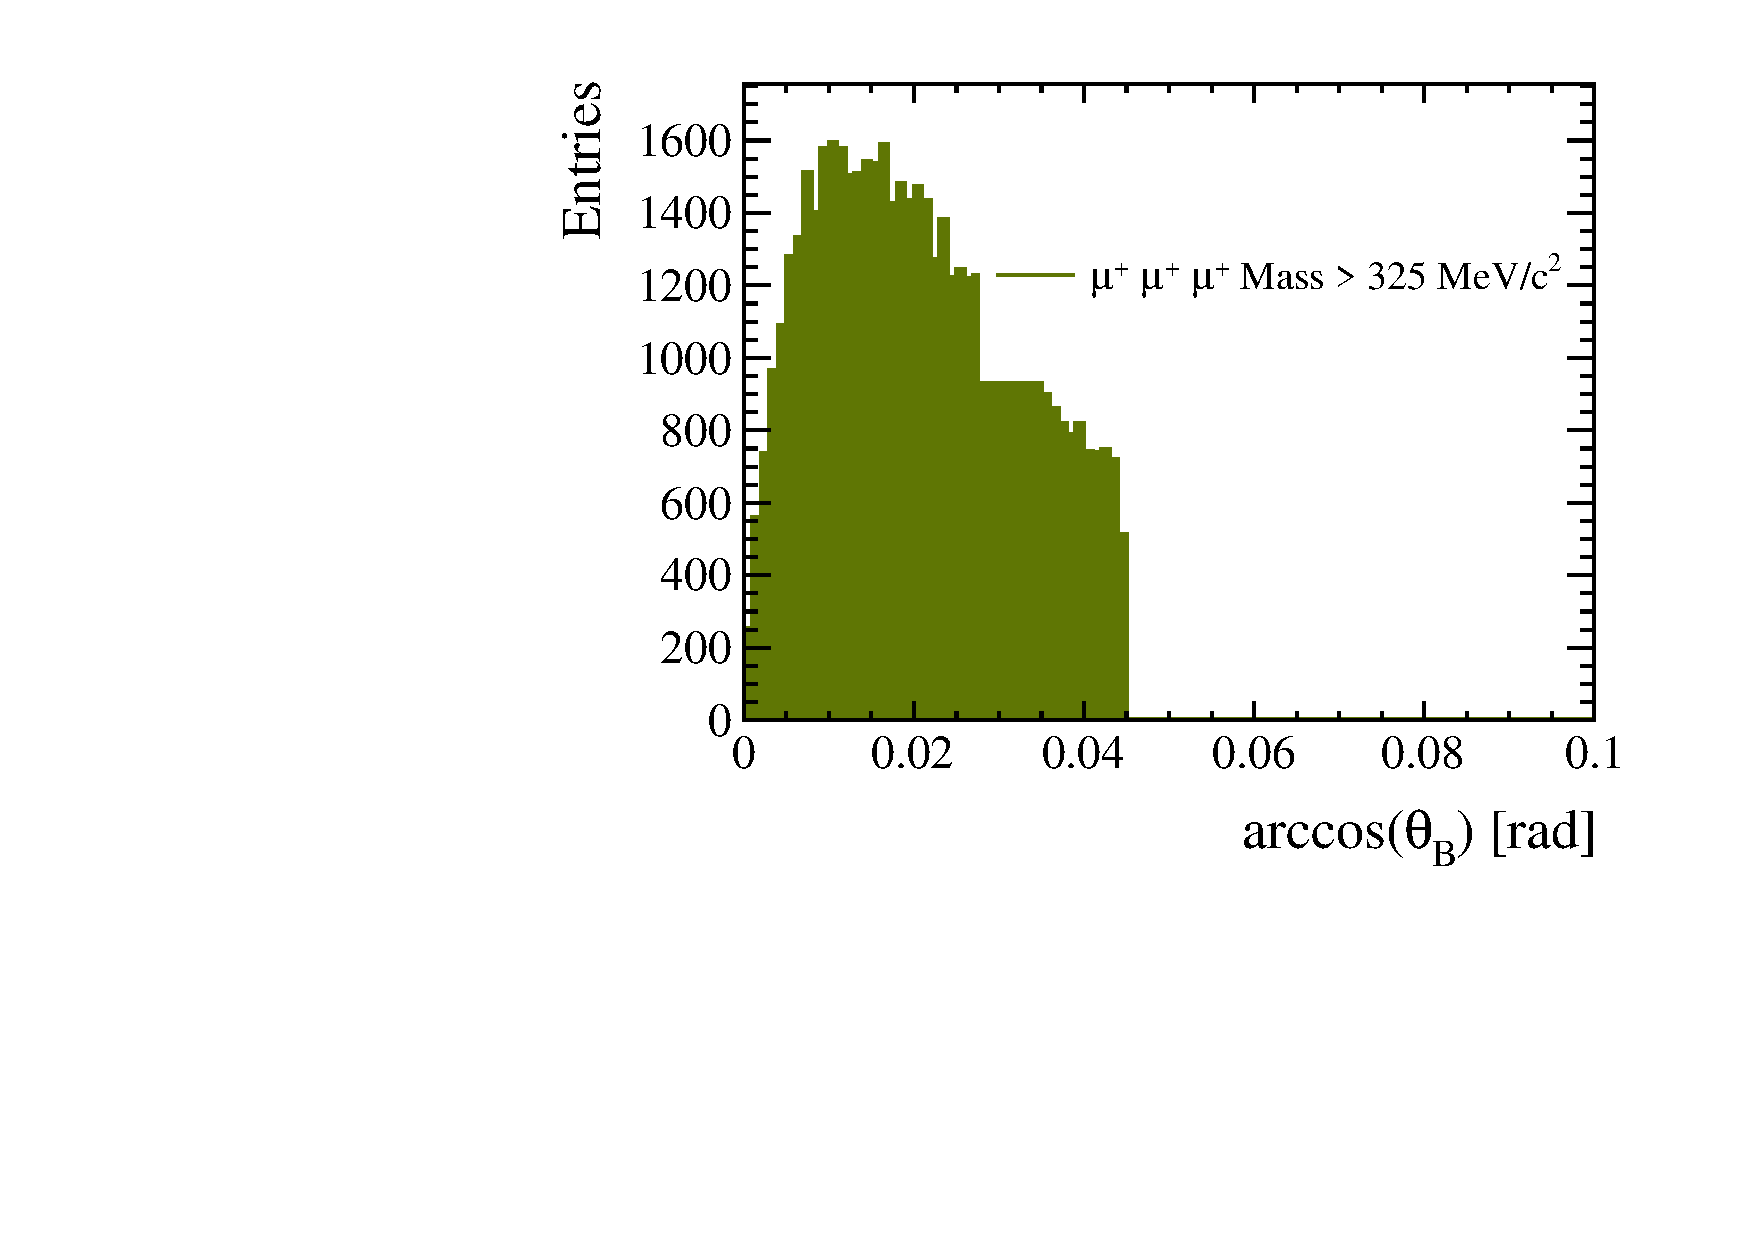
\includegraphics[width=0.5\linewidth]{trimuon/compnice_even_nicer_ONLY_STACKED_HIST_oneFILE_BplusDiranoclone.pdf}\put(-50,133){(b)}
	\caption{(a) Peaking clone distribution is visible as all of \textit{clone} tracks are collinear compared to (b) smooth no clone distribution for \gls{DIRA}.}
\label{fig:ClonesDIRA}
%\vspace*{-1.0cm}
\end{figure}

Hence, missing $p_{T}$ in the direction of the flight can be calculated using \gls{DIRA} and typical $p$,

\begin{equation}
	p_{T}=100\gevc \times \sin(0.0007)=0.7\gevc.
	\label{eq:mispt}
\end{equation}

Hence corrected mass $M_{corr} = \sqrt{{M}^{2} + |p^{2}_{T}|} + |p_{T}| = 4.2 \gevcc$, using missing $p_{T}$ from \autoref{eq:mispt} and visible mass of \textit{clones} from \autoref{eq:invmass}.


In order to suppress these tracks in analysing \Bmumumu, where two muons have the same sign, any distinguishing features mentioned could be used. But the most powerful \gls{PID}-wise is requiring \texttt{nShared==0}, as this requirement removes all of the clones, as seen in \autoref{fig:ClonesnShared}.

%\newline In order to keep the signal efficiency high in 2016 data, as shown in Table ~\ref{tab:Reason}, softer condition ,$\texttt{nShared}<2$, is applied.

\begin{figure}[h!]
\centering
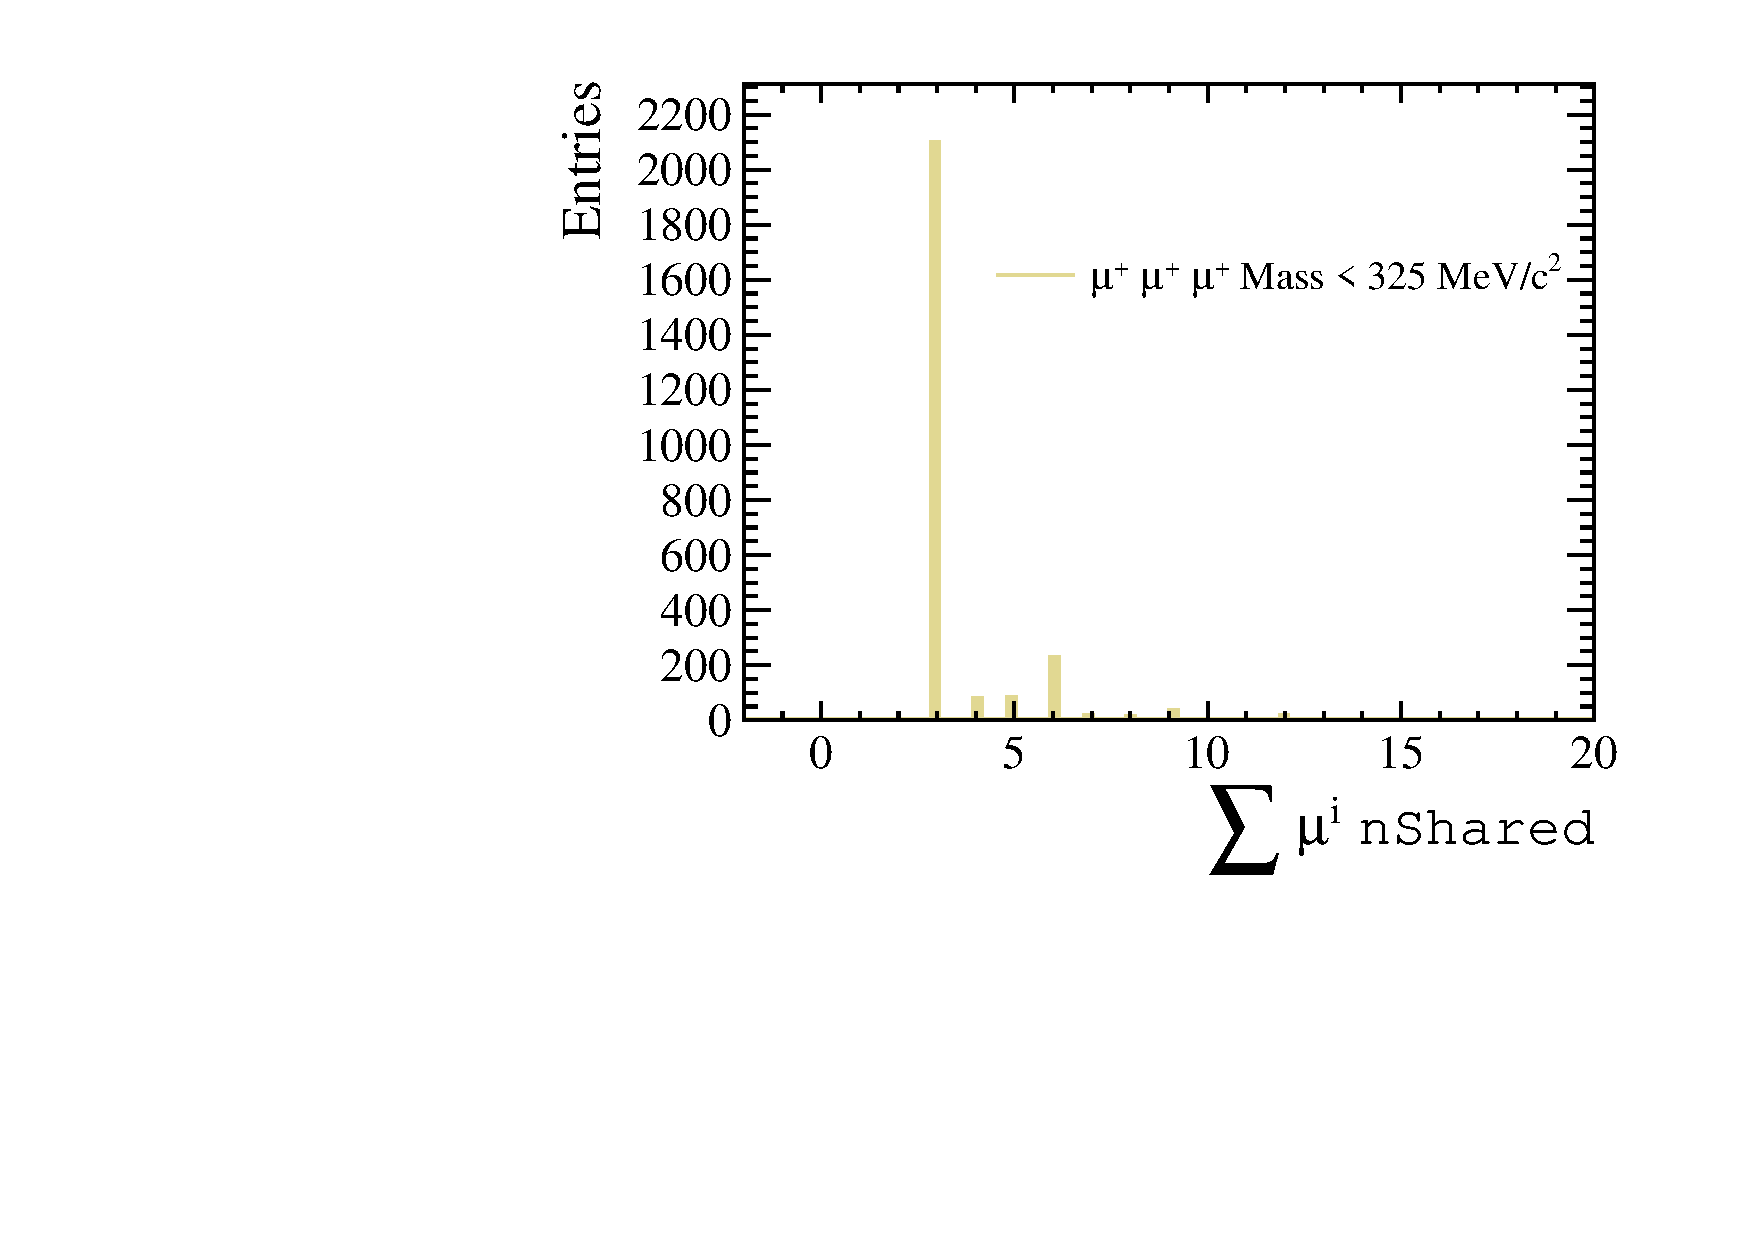
\includegraphics[width=0.5\linewidth]{trimuon/compnice_even_nicer_ONLY_STACKED_HIST_oneFILE_sumnSharedclone.pdf}\put(-50,133){(a)}
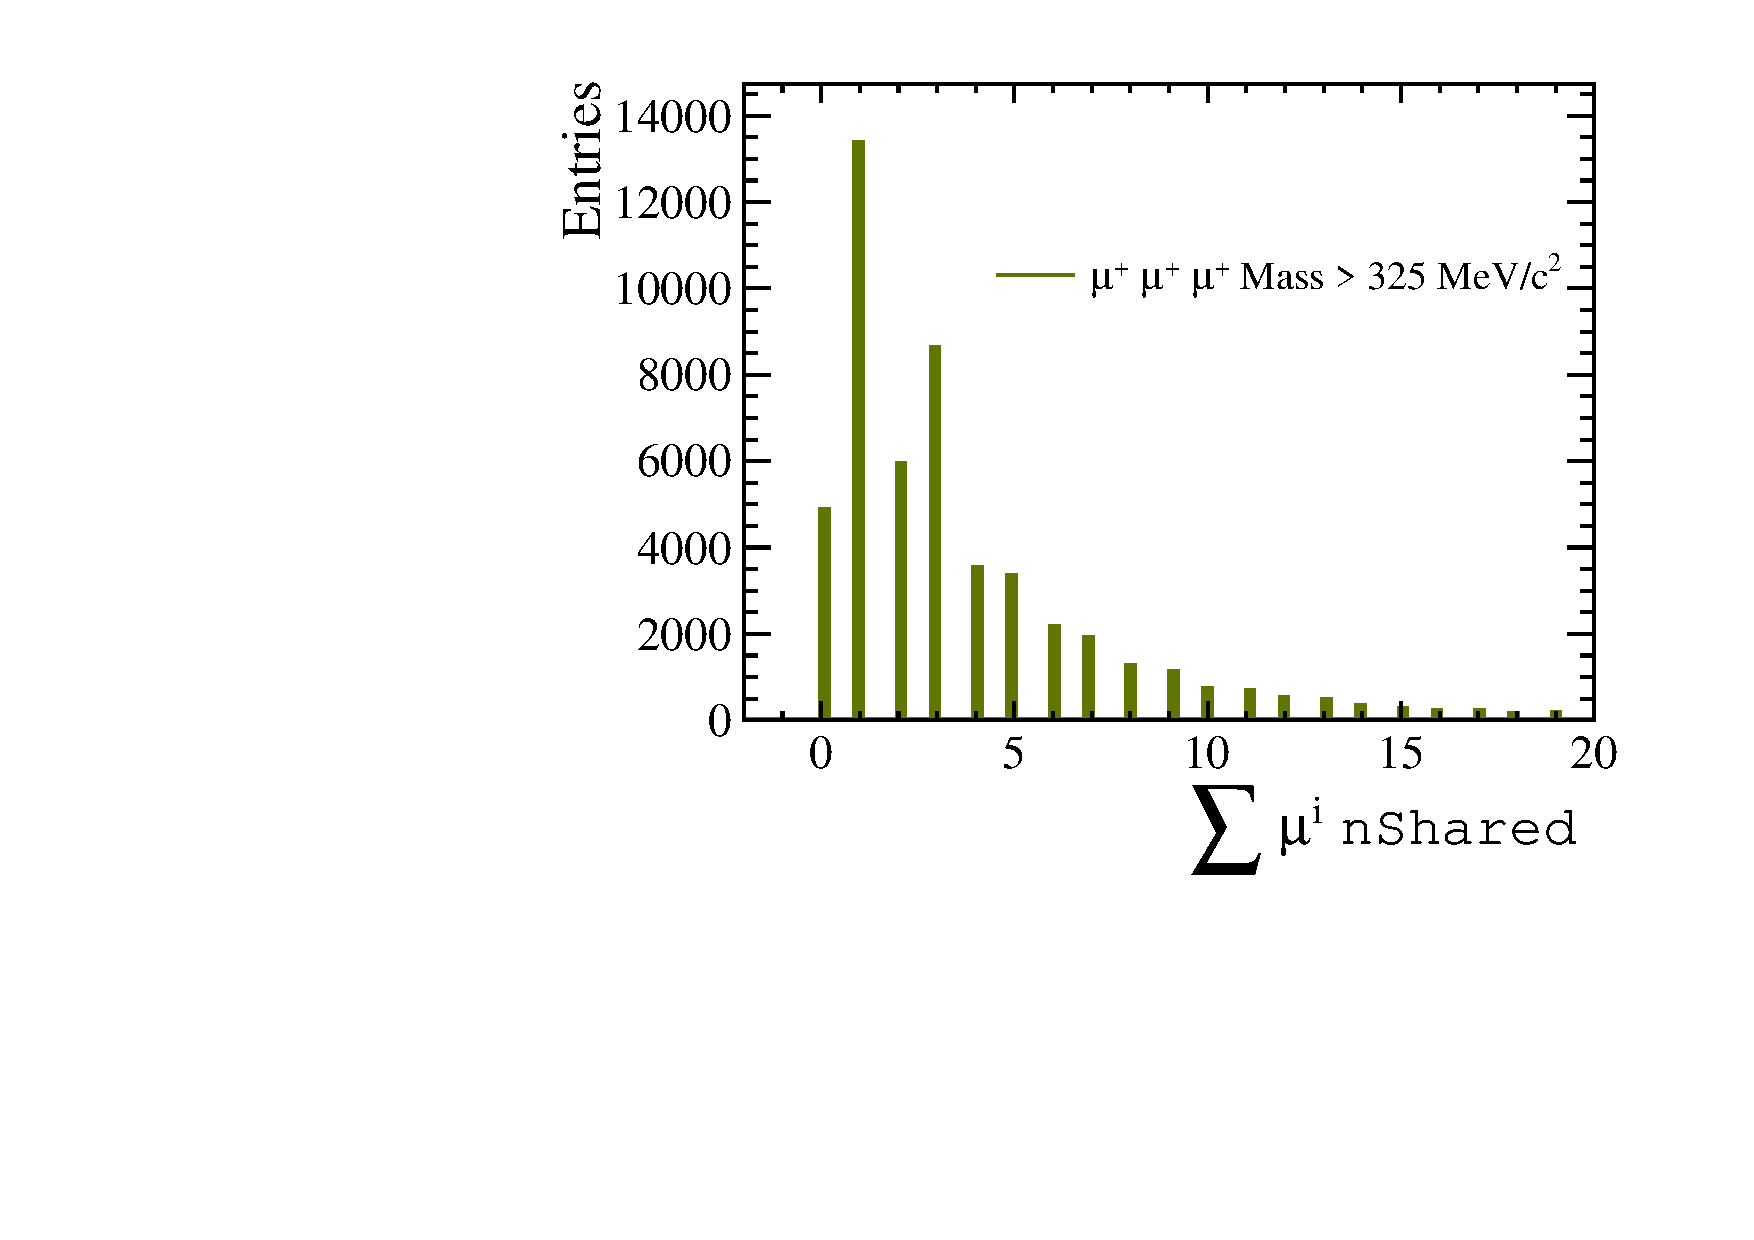
\includegraphics[width=0.5\linewidth]{trimuon/compnice_even_nicer_ONLY_STACKED_HIST_oneFILE_sumnSharednoclone.pdf}\put(-50,133){(b)}
	\caption{(a) Clone and (b) no clone distribution for sum of all muon \texttt{nShared}. Since in this case the clones are of each other, for clone there is clear peak at three. }
\label{fig:ClonesnShared}
%\vspace*{-1.0cm}
\end{figure}

\section{Probability of $K/\pi$ $\rightarrow \mu$ misidentification at LHCb \mybox{ULRIK}}

Usually, in order to estimate background coming from misidentification of species into muons in the detector, data samples with \textit{non-muon} (identified not to be muons) tracks are obtained. They are assigned parametrically probabilities of misid rates from some specific control samples, which were discussed in \autoref{RICHperf}. However, three muon signature will induce problems for \gls{PID} variables that are correlated with the number of muons in the detector and other control samples need to be used.

\subsection{Specific control sample for $K/\pi$ $\rightarrow \mu$ misid rates \mybox{ULRIK}}
\label{extraction}
At LHCb, \texttt{PIDCalib} package can usually provide misID and ID rates obtained from standard $K/\pi$ control samples $D^{*+}(\rightarrow D^{0}(\rightarrow \underline{K^{+} \pi^{-}}) \pi^{+})$. These statistically populated background-free \textit{sWeighted} samples, for which it is possible to extract misID and ID rates as a function of kinematics given certain \gls{PID} criteria, do not have other muons in the final state. 

More specifically, the topology of the mis-ID background component, which is two real muon tracks with an additional \textit{fake} muon track is very different to \texttt{PIDCalib} sample $D^{*+}(\rightarrow D^{0}(\rightarrow \underline{K^{+} \pi^{-}}) \pi^{+})$, where there are no muons in the final state. This influences rest of misID rates as some of the \gls{PID} variables are strongly correlated with number of muons in the decay, due to the fact that the mis-identified particle can share hits with other muons in the rest of the decay. This should be reflected mostly in high momenta region, where the three particles tend to be collimated and share hits most often.

For this reason, an alternative sample that is also be statistically populated background-free, $B^{0} \rightarrow J/\psi(\rightarrow \mu^{+} \mu^{-}) K^{*}(\rightarrow \underline{K^{+} \pi^{-}})$. It mimics the two real muon plus fake muon correctly and will be used to obtain pion and kaon misID probabilities.
% This is a clean decay that can be fit to obtain \textit{sWeights} to measure PID efficiencies. Moreover, its the signal topology and kinematics are much closer to the actual mis-ID backgroundcomponent than
% that of the PIDCalib control samples.

\subsection{Selection for $B^{0} \rightarrow J/\psi(\rightarrow \mu^{+} \mu^{-}) K^{*}$ \mybox{ULRIK} }
Data samples for each year of data taking were obtained from \textit{stripping} dedicated to look for this type of decay, but with both kaon and pion having no particle identification applied, which ensures that \gls{PID} performance of different variables can be studied. Some initial selection was applied together with more stringent \Bmumumu selection including trigger (but on $J/\psi$ candidate rather than $B$). Finally to remove most of the backgrounds that still pollute the signal samples following selection summarized in Table ~\ref{tab:cleanjpsikst} is used.


\begin{table}[h!]
\begin{center}
\begin{tabular}{ l  l }
Idea  & Cut  \\ \hline
ID $K^{*}$ & $|$ m(K$\pi$) - m$_{PDG}(K^{∗}_{0})$ $|$ $ <100$ \mevcc \\
Compatible with \texttt{PIDCalib} &  for K,$\pi$ , p$_{T} > 250$ \mevc\\
Compatible with \texttt{PIDCalib} &  for $\mu$ , p$_{T} > 800$ \mevc \\
Muon swap veto & $|$ m((h $\rightarrow \mu$ )$\mu$) - m$_{PDG}$(J/$\psi$)$|$ $> 60$ \mevcc \\
	Veto $B^{+}\rightarrow K^{+}\mu^{+}\mu^{-}$ & max(m($K^{+}\mu^{+}\mu^{-}$)), m($(\pi^{+} \rightarrow K^{+})\mu^{+}\mu^{-})$) $< 5100$ \mevcc\\
Veto $B^{0}_{s}\rightarrow \phi \mu^{+} \mu^{-} $ & m(K($\pi\rightarrow$ K)) $>1040$ \mevcc \\
ID muons & mu1$\_$ProbNNmu$>$0.5 and mu2$\_$ProbNNmu$>$0.5 \\
\hline
For kaon misID rates: & \\
ID pion & DLLK $<$ 0 DLLp $<$ 0 and \texttt{IsMuon==0}\\
\hline
For pion misID rates: & \\
ID kaon & DLLK $>$ 0 and DLLK-DLLp $>$ 0 and \texttt{IsMuon==0} \\
\hline
\end{tabular}
\end{center}
\caption{Offline selection for $B^{0} \rightarrow J/\psi(\rightarrow \mu^{+} \mu^{-}) K^{*}$ decay.}
\label{tab:cleanjpsikst}
\end{table}


\subsection{Fitting Strategy for $B^{0} \rightarrow J/\psi(\rightarrow \mu^{+} \mu^{-}) K^{*}$ decay \mybox{ULRIK}}
After all the selection, the residual background needs to be modelled. 

The signal component, $B^{0} \rightarrow J/\psi K^{*}$, is obtained by fixing the shape from simulation apart from mean $\mu$ and width $\sigma$. It is fitted with double-sided Hypatia function \cite{Santos:2013gra} (more in \autoref{IP}).

Background that peaks in the upper mass sideband, coming from heavier $B^{0}_{s}$, $\bar{B}^{0}_{s} \rightarrow J/\psi (\rightarrow \mu^{+} \mu^{-}) K^*(\rightarrow \underline{K^{+} \pi^{-}})$ is also modelled using simulation, using the same function as a signal but with offset of $\mu$ by PDG difference between $B^{0}_{s}$ and $B^{0}$.

It is also possible that kaons and pions are swapped between themselves. Background coming from $K \leftrightarrow \pi$ swaps is modelled from simulation where mass hypotheses were swapped. Its distribution is fitted with double sided Crystal Ball function \cite{Skwarnicki:1986xj} (more in \autoref{CB}).

Possibility of misidentified background comes from decay of $\Lambda_{b} \rightarrow K^{-} p \mu^{+} \mu^{-}$ where proton is misidentified as pion. This background is modelled from simulation and fitted with \texttt{RooKeys} p.d.f (more in \autoref{RK}).

And finally combinatorial component is modelled by the exponential function.

In order to obtain $K/\pi$ misid probabilities fit to $\mu^{+} \mu^{-} \pi^{+} K^{-}$ mass between 5150 - 5450 \mevcc was performed, where all of the yields for different components are left floating. Moreover, mass of $J/\psi$ was \textit{constrained} to its nominal mass, known as \textit{mass constraint}, which will yield new estimates for track parameters of the final state particles, from which a new kinematic refit is done.

Actual extraction of the misid rate was obtained using statistical subtraction of background, also known as \textit{sPlot} technique. The same is used in \texttt{PIDCalib} package. It was cross-checked with \textit{fit twice method}, because \textit{sPlot} technique relies on the fact that there is no correlation between the between the control variables ($p$, $\eta$) and the discriminating variable (invariant mass) for both signal and background. This assumption may not be true especially for background, and it can introduce biases.

The \textit{fit twice method} consists of fitting $B^{0} \rightarrow J/\psi(\rightarrow \mu^{+} \mu^{-}) K^{*}$ before and after \gls{PID} requirement in a given kinematic ($p$, $\eta$) bin separately. Misid probabilities are then then obtained as a ratio of signal yields arising from these two fits.

In the \textit{sPlot} method, the invariant mass distribution is fitted once and each event is assigned \textit{sWeights}, probabilities that a given event is a signal-like or a background-like. Then, through \textit{sPlot} technique, background is subtracted. The misid probabilities are then obtained by looking at sum of all \textit{sWeights} in each bin.

It was shown that these two methods yields very similar results, hence,
for purposes of \Bmumumu analysis \textit{sWeight} values will be used. Fits to Run \Rn{1} and Run \Rn{2} data can be seen in ~\autoref{fig:JpsiKst}.
%IF YOU WANT TO CHANGE THE PLOTS HAVE A LOOKHERE /vols/lhcb/ss4314/fitjpsikst/fitjpsikst_idKAON_includeswaps_automatize_master_sweight_cinMuonAc_NOghostprob_mydefbin_onnlyONEbinINeta_2016_newPIDopt/NOFCME/ there is mainPLOTonly function
\begin{figure}[H] 

\center
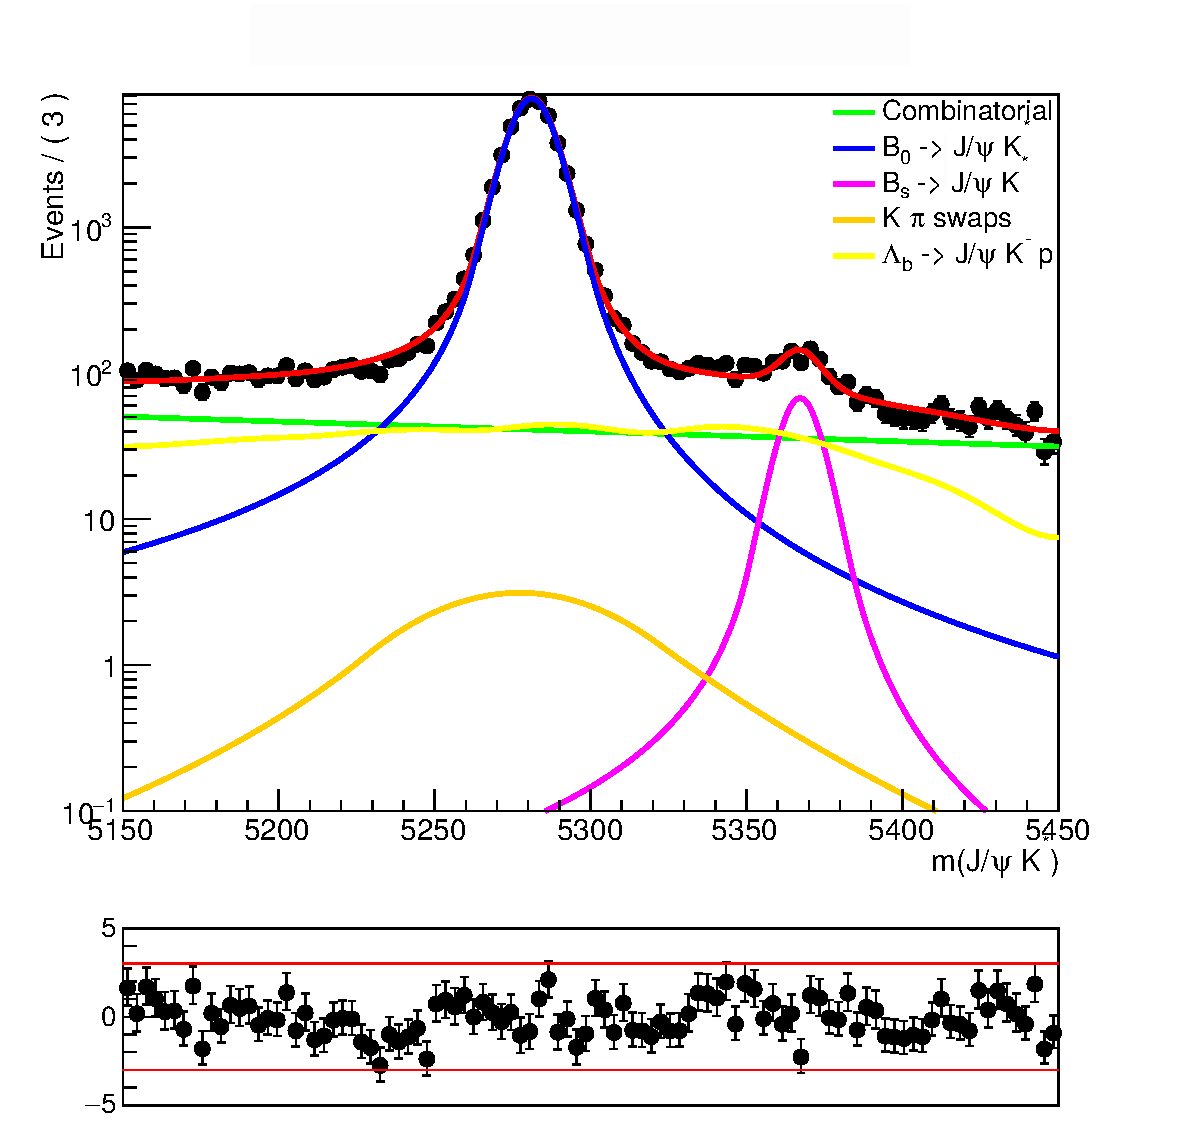
\includegraphics[width = 0.5\textwidth]{figs/trimuon/jpsikst/2011/kaonmisid2011_new.pdf}\put(-150,100){(a) 49K events }%
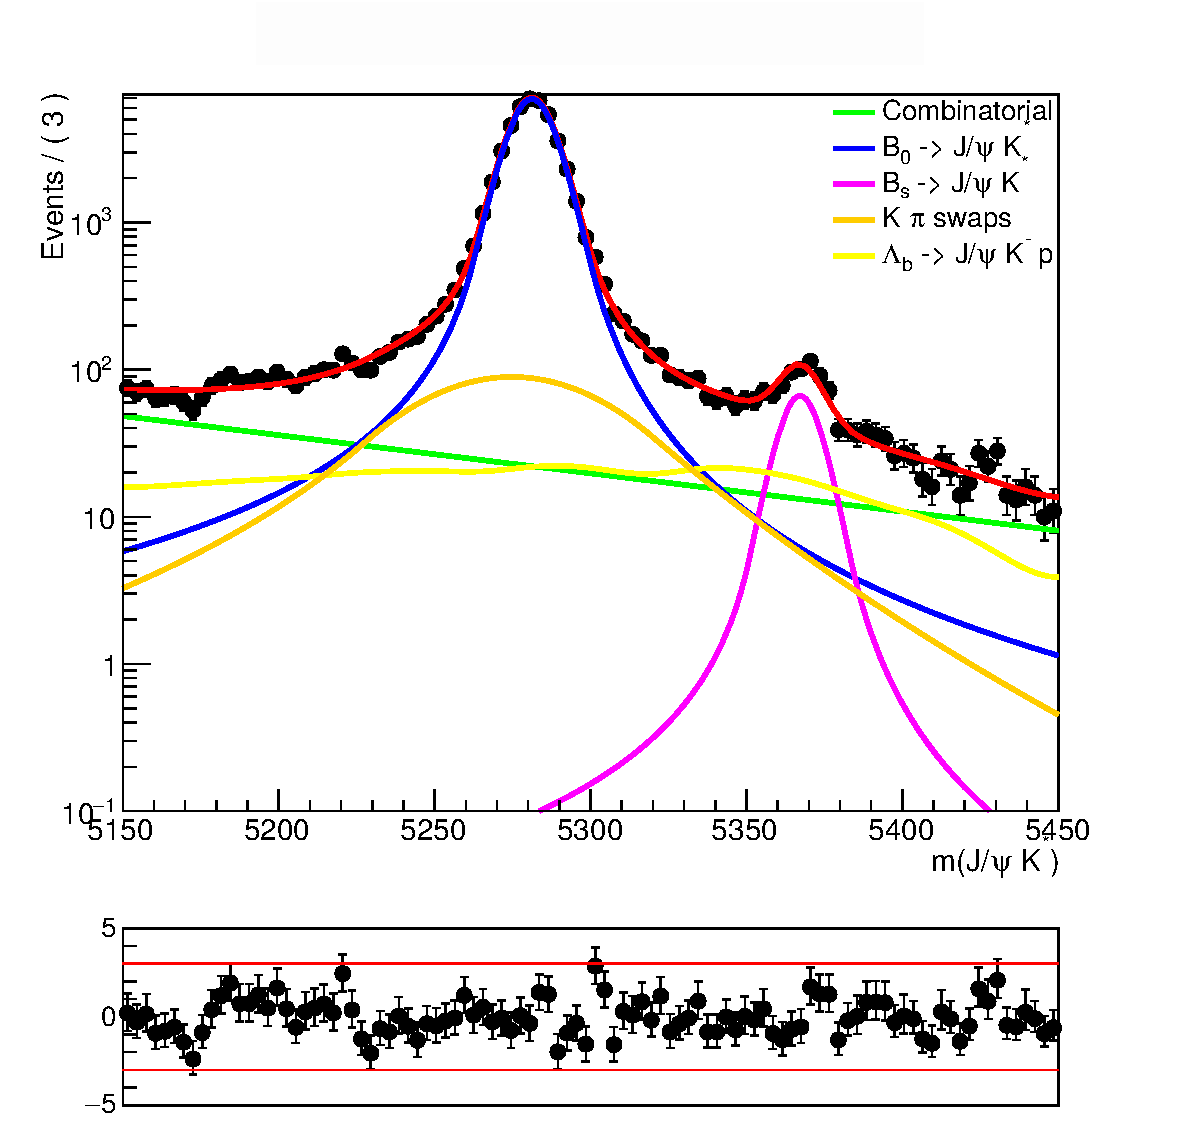
\includegraphics[width = 0.5\textwidth]{figs/trimuon/jpsikst/2011/pionmisid2011_new.pdf}\put(-150,100){(b) 46K events}
\newline
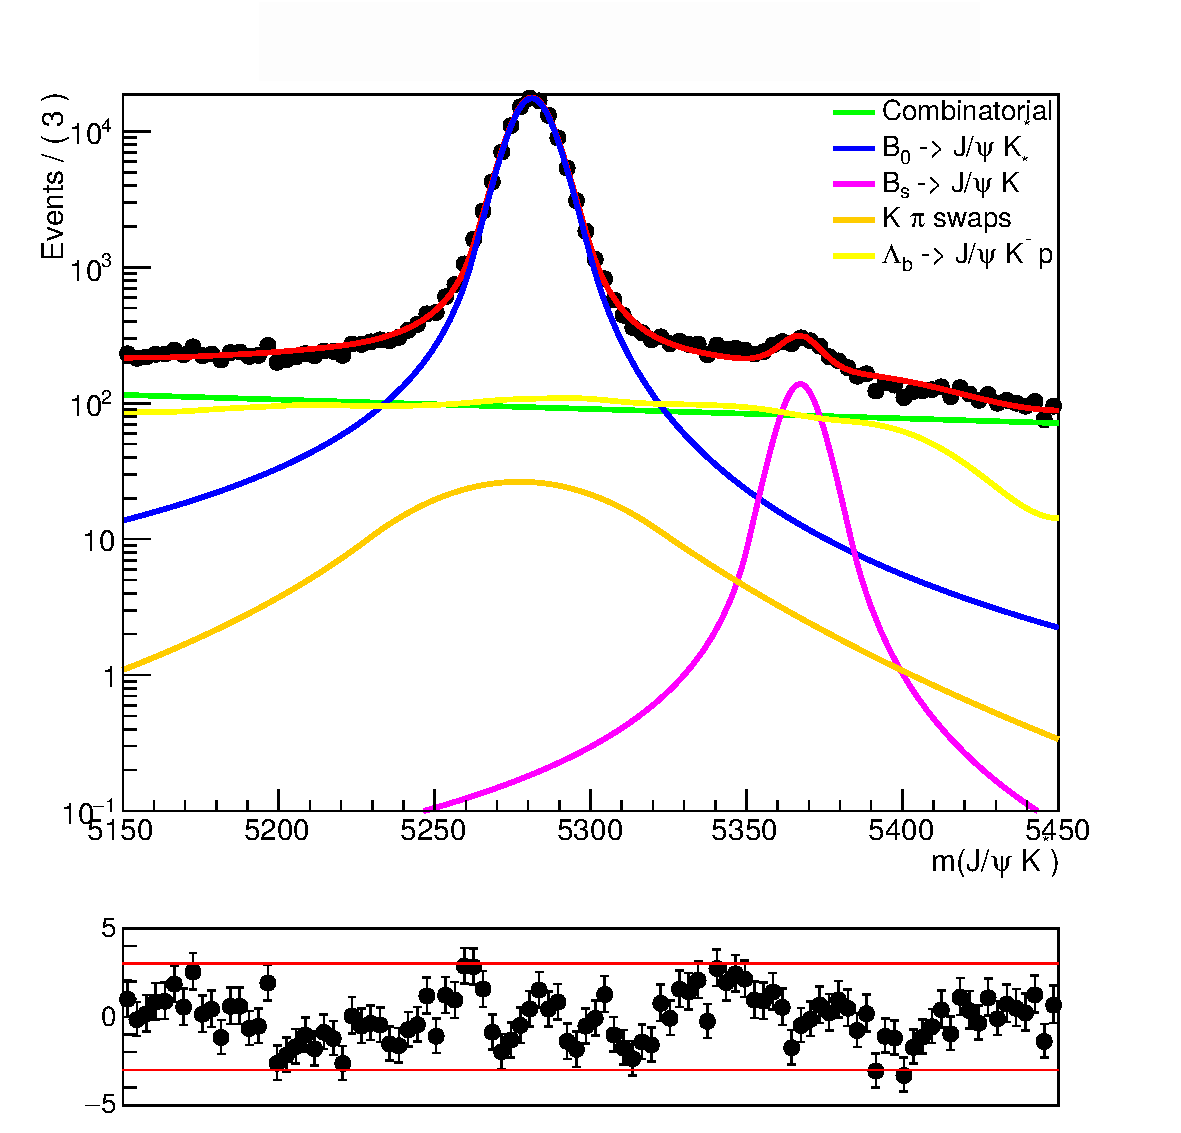
\includegraphics[width = 0.5\textwidth]{figs/trimuon/jpsikst/2012/KaonMisid_new.pdf}\put(-150,100){(c) 112K events }%
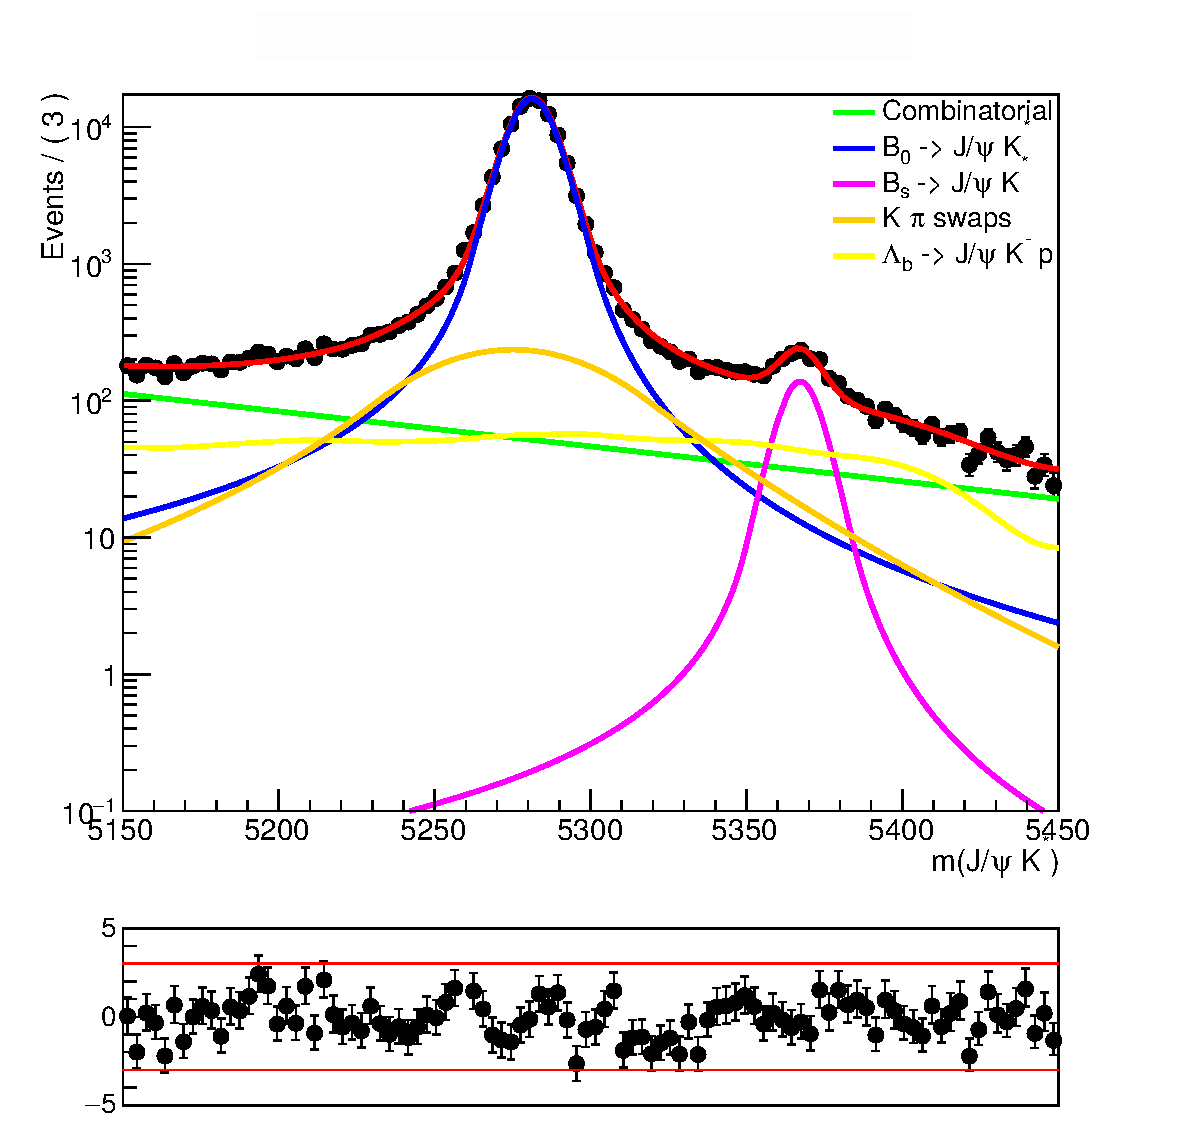
\includegraphics[width = 0.5\textwidth]{figs/trimuon/jpsikst/2012/PiMisid_new.pdf}\put(-150,100){(d) 107K events}
\newline
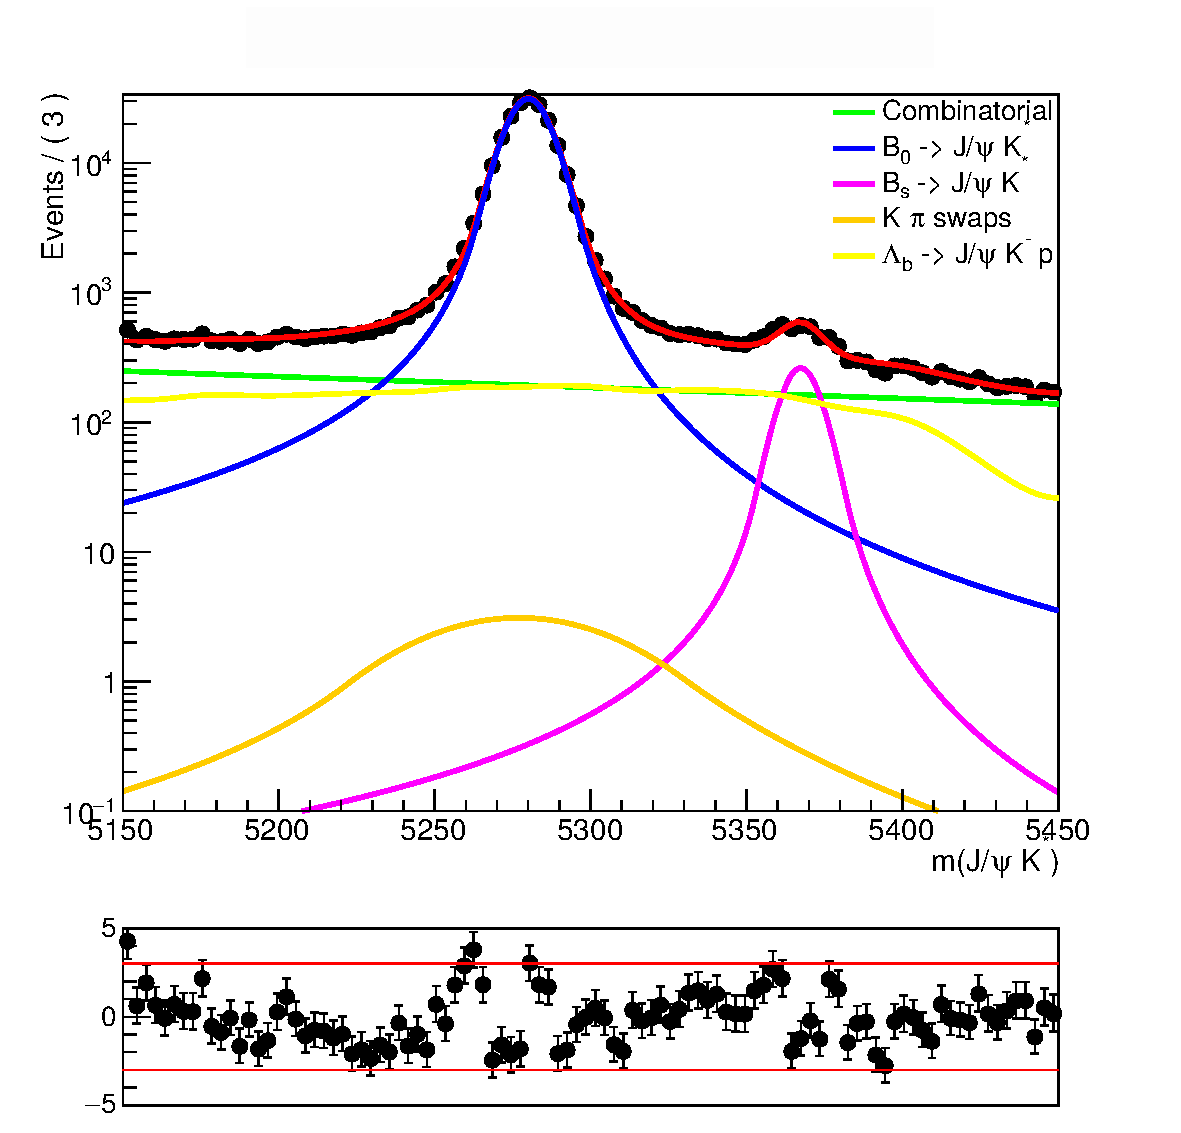
\includegraphics[width = 0.5\textwidth]{figs/trimuon/jpsikst/2016/kaonmisid2016_new.pdf}\put(-150,100){(e) 205K events}%
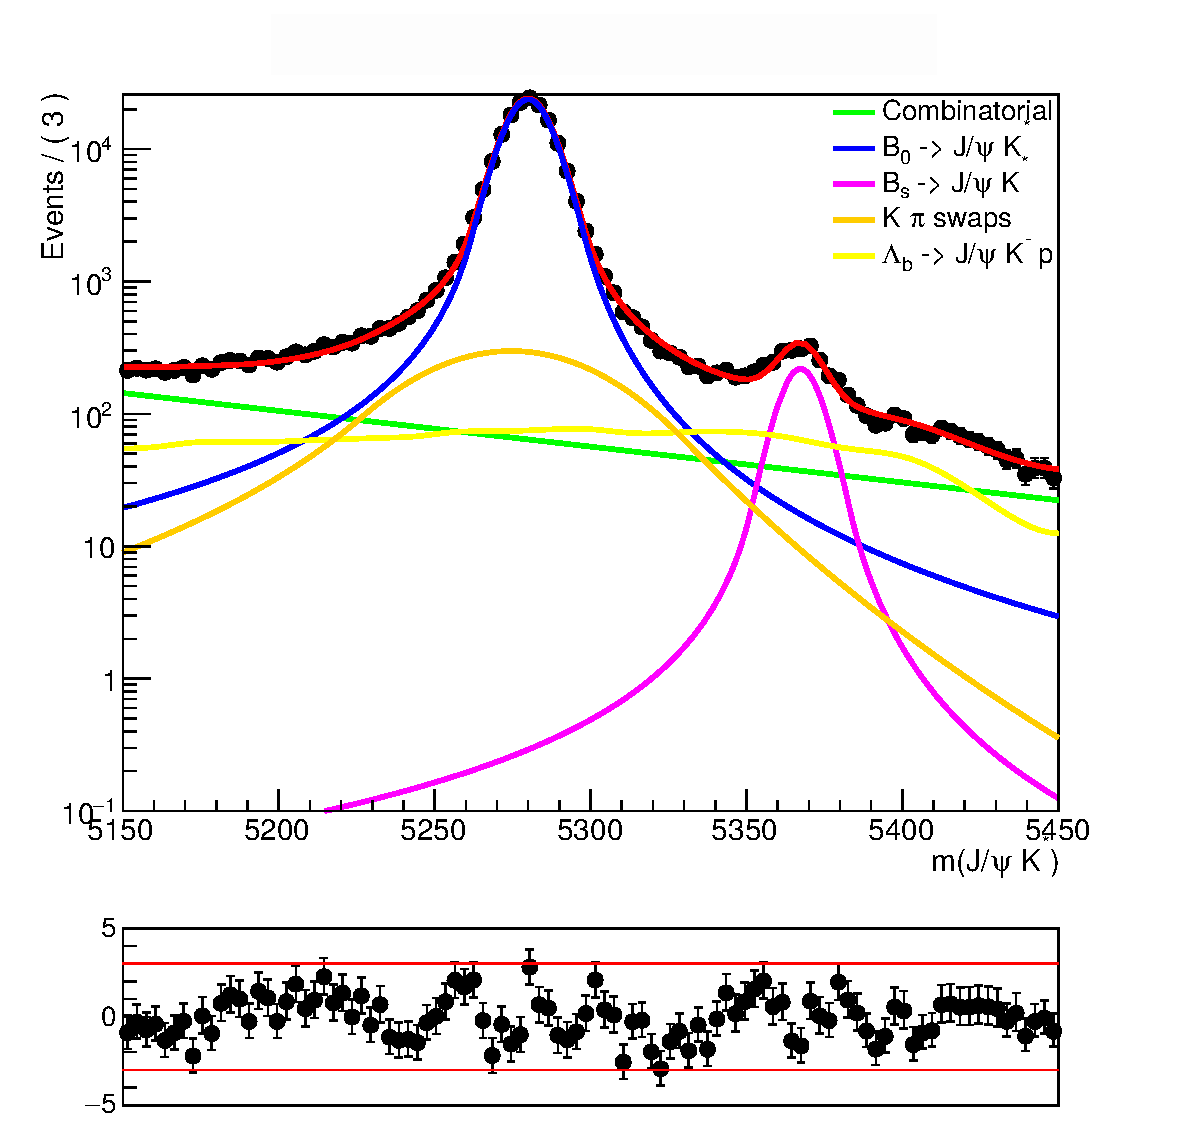
\includegraphics[width = 0.5\textwidth]{figs/trimuon/jpsikst/2016/pionmisid2016_new.pdf}\put(-150,100){(f) 161K events}
	\caption{Fit to constrained $J/\psi(\rightarrow \mu^{+} \mu^{-}) K^{*}(\rightarrow \pi^{+} K^{-})$ mass with all the components for (a)(b) 2011, (c)(d) 2012, (e)(f) 2016. On the left, fit to data with pion ID (giving kaon misid probabilities), on right data with kaon ID (pion misid rates).}
\label{fig:JpsiKst}
\end{figure}

\subsection{Results of $B^{0} \rightarrow J/\psi(\rightarrow \mu^{+} \mu^{-}) K^{*}$ control sample for $K/\pi$ $\rightarrow \mu$ misid rates \mybox{ULRIK}}
Using the \textit{sWeight} method, misID rates for $K/\pi$ can be obtained. In order to rule out that any disagreement of \gls{PID} performance is caused by the rest of the event (such as the different nature of the tracks) following check is performed. For both samples the probability of correctly identifying kaon is computed, given that only extrapolated tracks that fall within muon acceptance are considered. This is achieved by requiring that given kaon track has \texttt{InMuonAcceptance==1.0}. It can be seen in ~\autoref{tab:ROE} that the ID performance is the same across nearly all of the momentum range for kaons, showing that these kaons are good proxy for misID probability studies. The same check was done for pions tracks as well. 


\begin{table}[h!]
\small
\begin{center}
\begin{tabular}{ l  l  l  l  l  l }
	$p$ range [\mevc] & $D^{*+}(\rightarrow D^{0}(\rightarrow \underline{K^{+} \pi^{-}}) \pi^{+})$  & $B^{0} \rightarrow J/\psi(\rightarrow \mu^{+} \mu^{-}) K^{*}(\rightarrow \underline{K^{+} \pi^{-}})$  & Ratio  \\ \hline
3000 - 6000 &   0.77$\pm$0.0016 & 0.83$\pm$0.0047 & 1.1$\pm$0.0065 \\
6000 - 9300 &   0.93$\pm$0.00030 & 0.95$\pm$0.0019 & 1.0$\pm$0.0020 \\
9300 - 10000 &  0.96$\pm$0.00037 & 0.97$\pm$0.0031 & 1.0$\pm$0.0033 \\
10000 - 12600 &  0.97$\pm$0.00014 & 0.97$\pm$0.0017 & 1.0$\pm$0.0017 \\
12600 - 15600 &   0.98$\pm$0.00011 & 0.97$\pm$0.0017 & 0.99$\pm$0.0018 \\
15600 - 17500 &   0.98$\pm$0.00013 & 0.96$\pm$0.0024 & 0.98$\pm$0.0025 \\
17500 - 21500 &   0.98$\pm$8.9e-05 & 0.96$\pm$0.0018 & 0.98$\pm$0.0018 \\
21500 - 27000 &   0.98$\pm$7.8e-05 & 0.96$\pm$0.0018 & 0.98$\pm$0.0019 \\
27000 - 32000 &   0.98$\pm$8.8e-05 & 0.96$\pm$0.0024 & 0.98$\pm$0.0025 \\
32000 - 40000 &  0.98$\pm$8.0e-05 & 0.96$\pm$0.0022 & 0.98$\pm$0.0022 \\
40000 - 60000 &  0.97$\pm$7.5e-05 & 0.95$\pm$0.0021 & 1.0$\pm$0.0022 \\
60000 - 70000 &  0.96$\pm$0.00016 & 0.96$\pm$0.0043 & 1.0$\pm$0.0046 \\
70000 - 100000 &  0.95$\pm$0.00013 & 0.94$\pm$0.0044 & 0.99$\pm$0.0046 \\
\hline

\end{tabular}
\end{center}
\caption{\texttt{K$\_$InMuonAcc==1.0} shows the interpolation of $K$ tracks into muon chambers. It can be seen that both samples agree with each other, meaning that the rest of the event information is the same for both samples. This measurement is in a bin $1.5<\eta<5.0$.}
\label{tab:ROE}
\end{table}


Hence using \texttt{InMuonAcc==1.0} tracks for both pion and kaon allows to perform study of the misID probabilities within the two calibration samples.
In ~\autoref{fig:JpsiKnew}, $\pi \rightarrow \mu$ misID probability for different \gls{PID} hypotheses are studied. As it can be noticed, the more stringent the muon selection on the pion track the lower the probability of misidentification. On the right, the ratio of the misID probabilities between two samples show particular trend. 


\begin{figure}[h!]
\center
%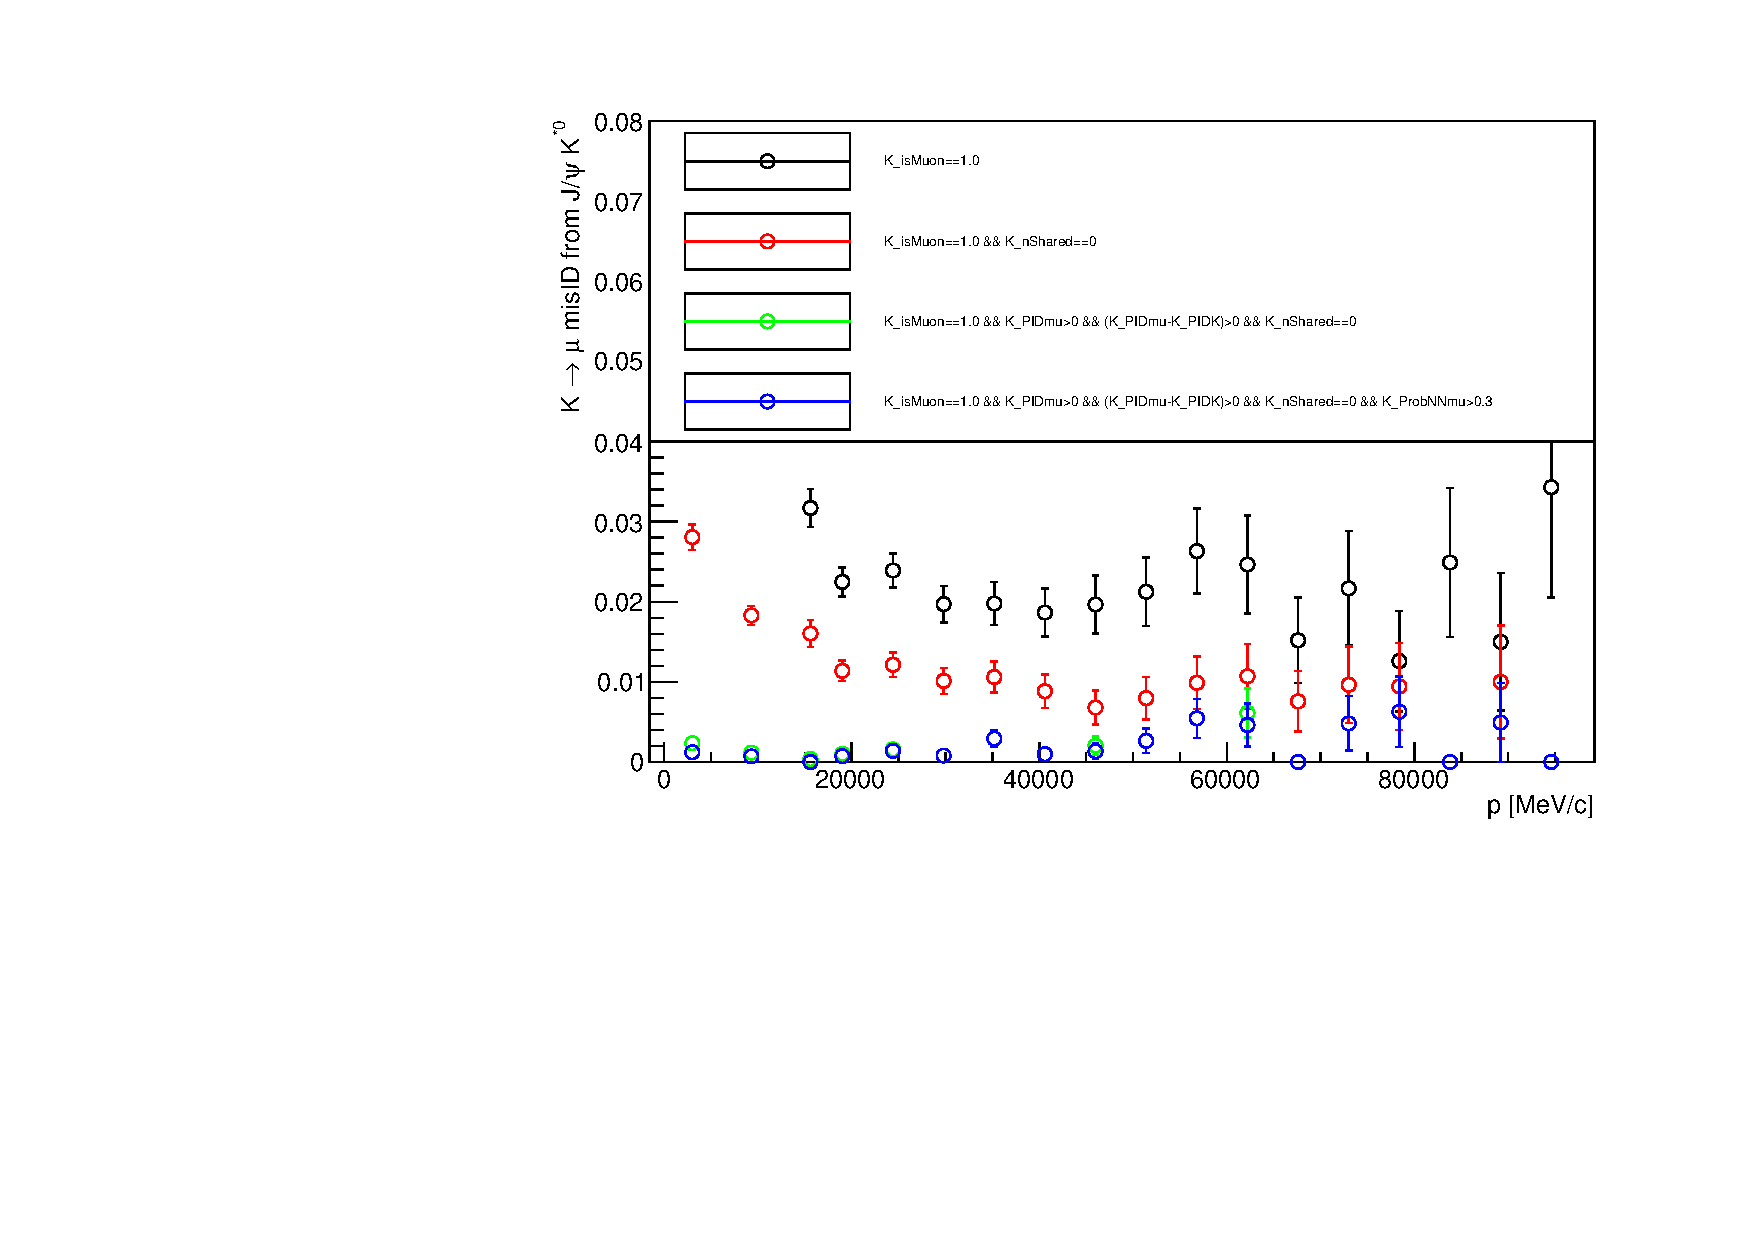
\includegraphics[width = 0.55\textwidth]{figs/trimuon/jpsikst/2012/Visualize_Weights_KaonMisid_2011_small.pdf}\put(-50,133){(a)}%
		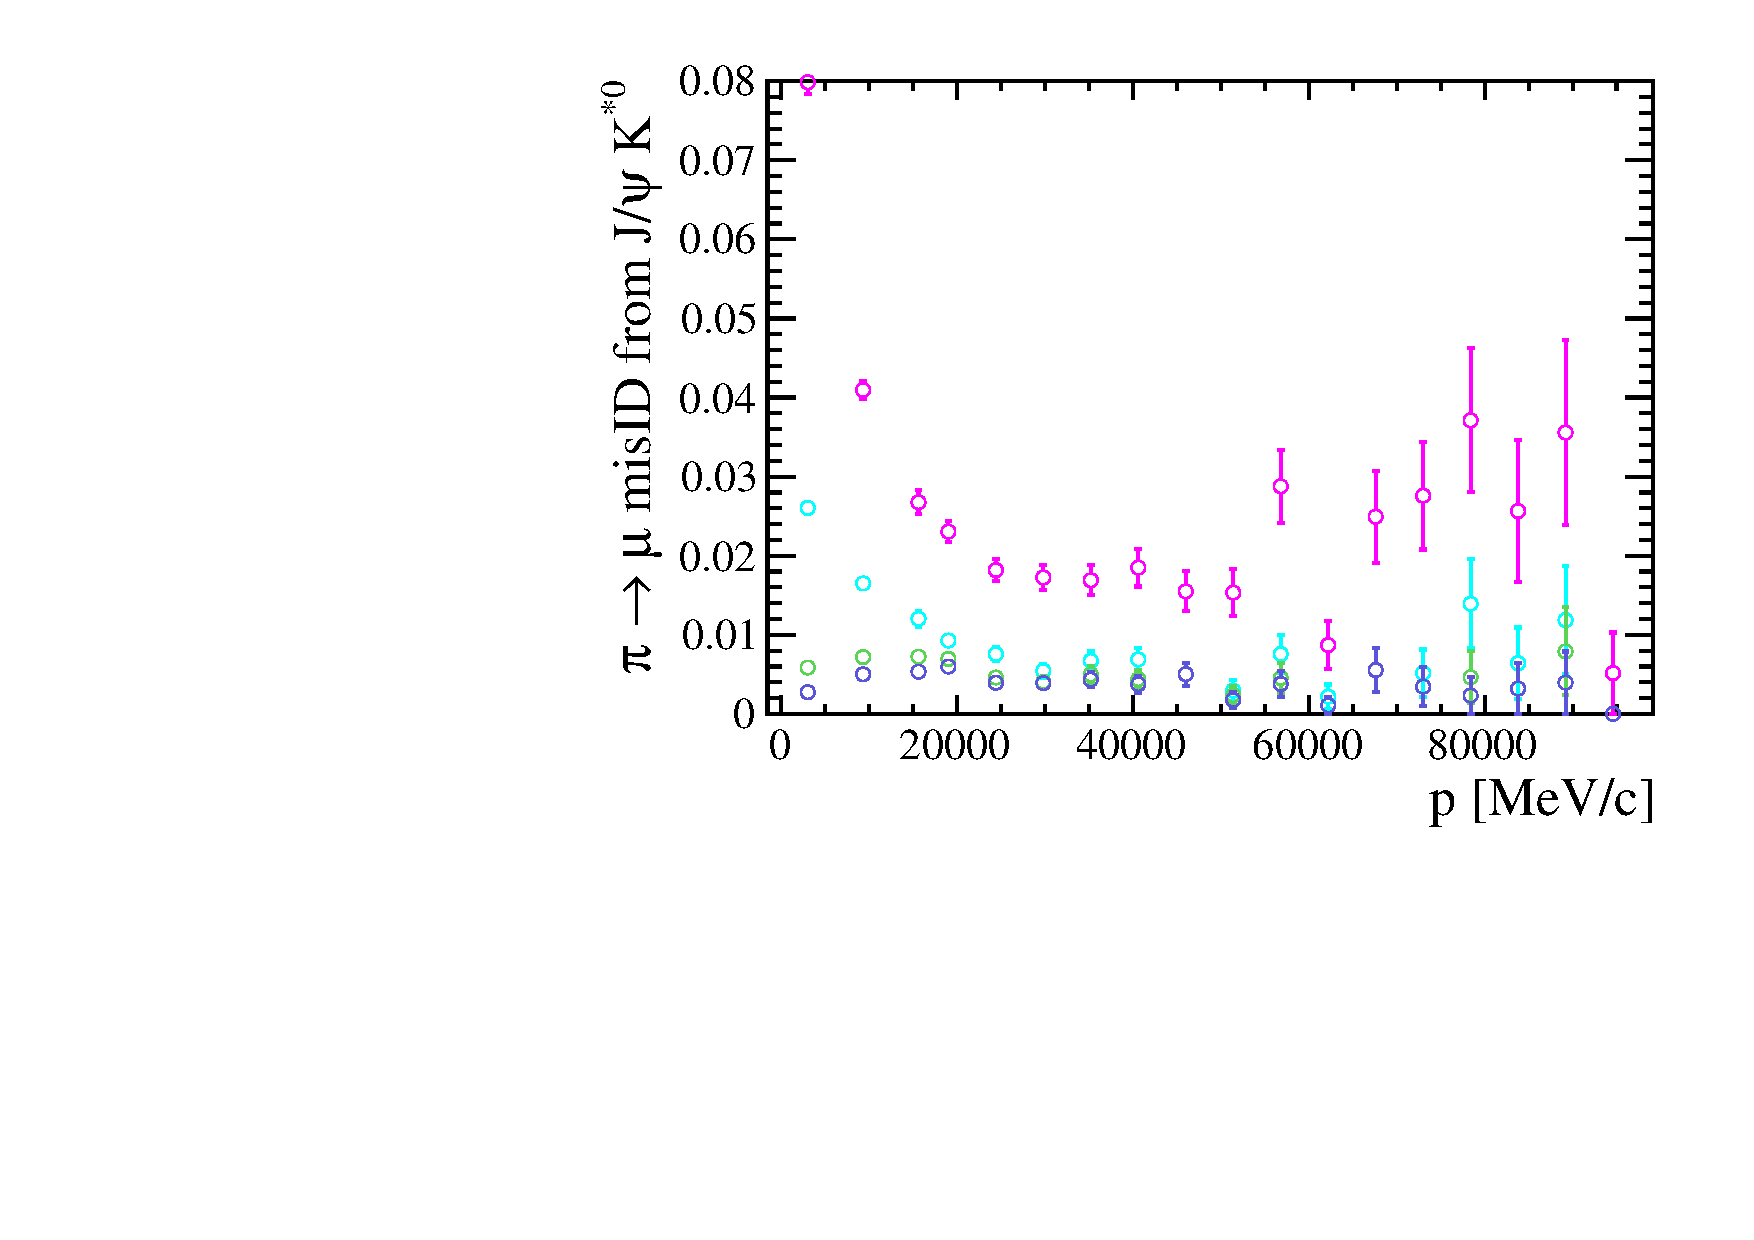
\includegraphics[width = 0.5\textwidth]{figs/trimuon/jpsikst/2012/Visualize_Weights_PionMisid_2012_small_thesis.pdf}\put(-50,133){(a)}
%		\newline
%		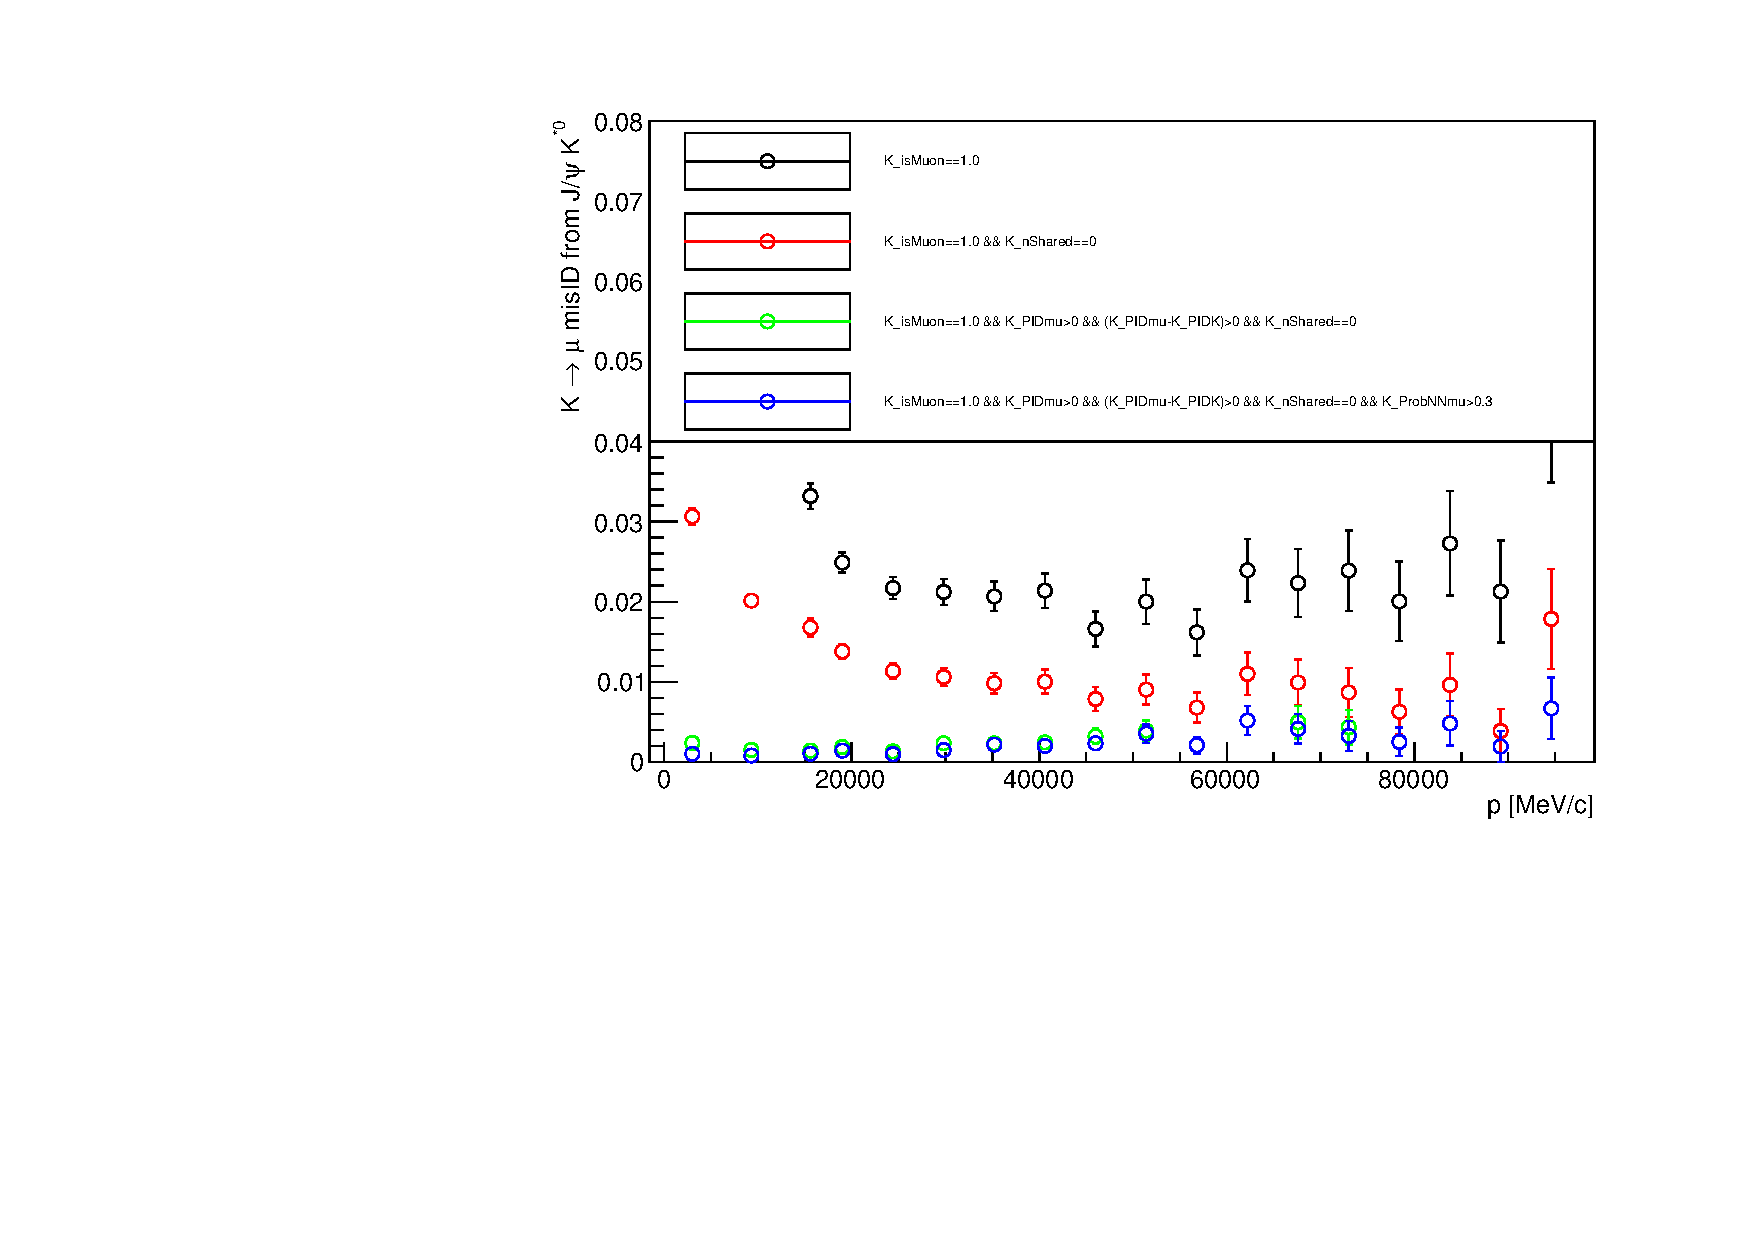
\includegraphics[width = 0.55\textwidth]{figs/trimuon/jpsikst/2012/Visualize_Weights_KaonMisid_small.pdf}\put(-50,133){(c)}%
		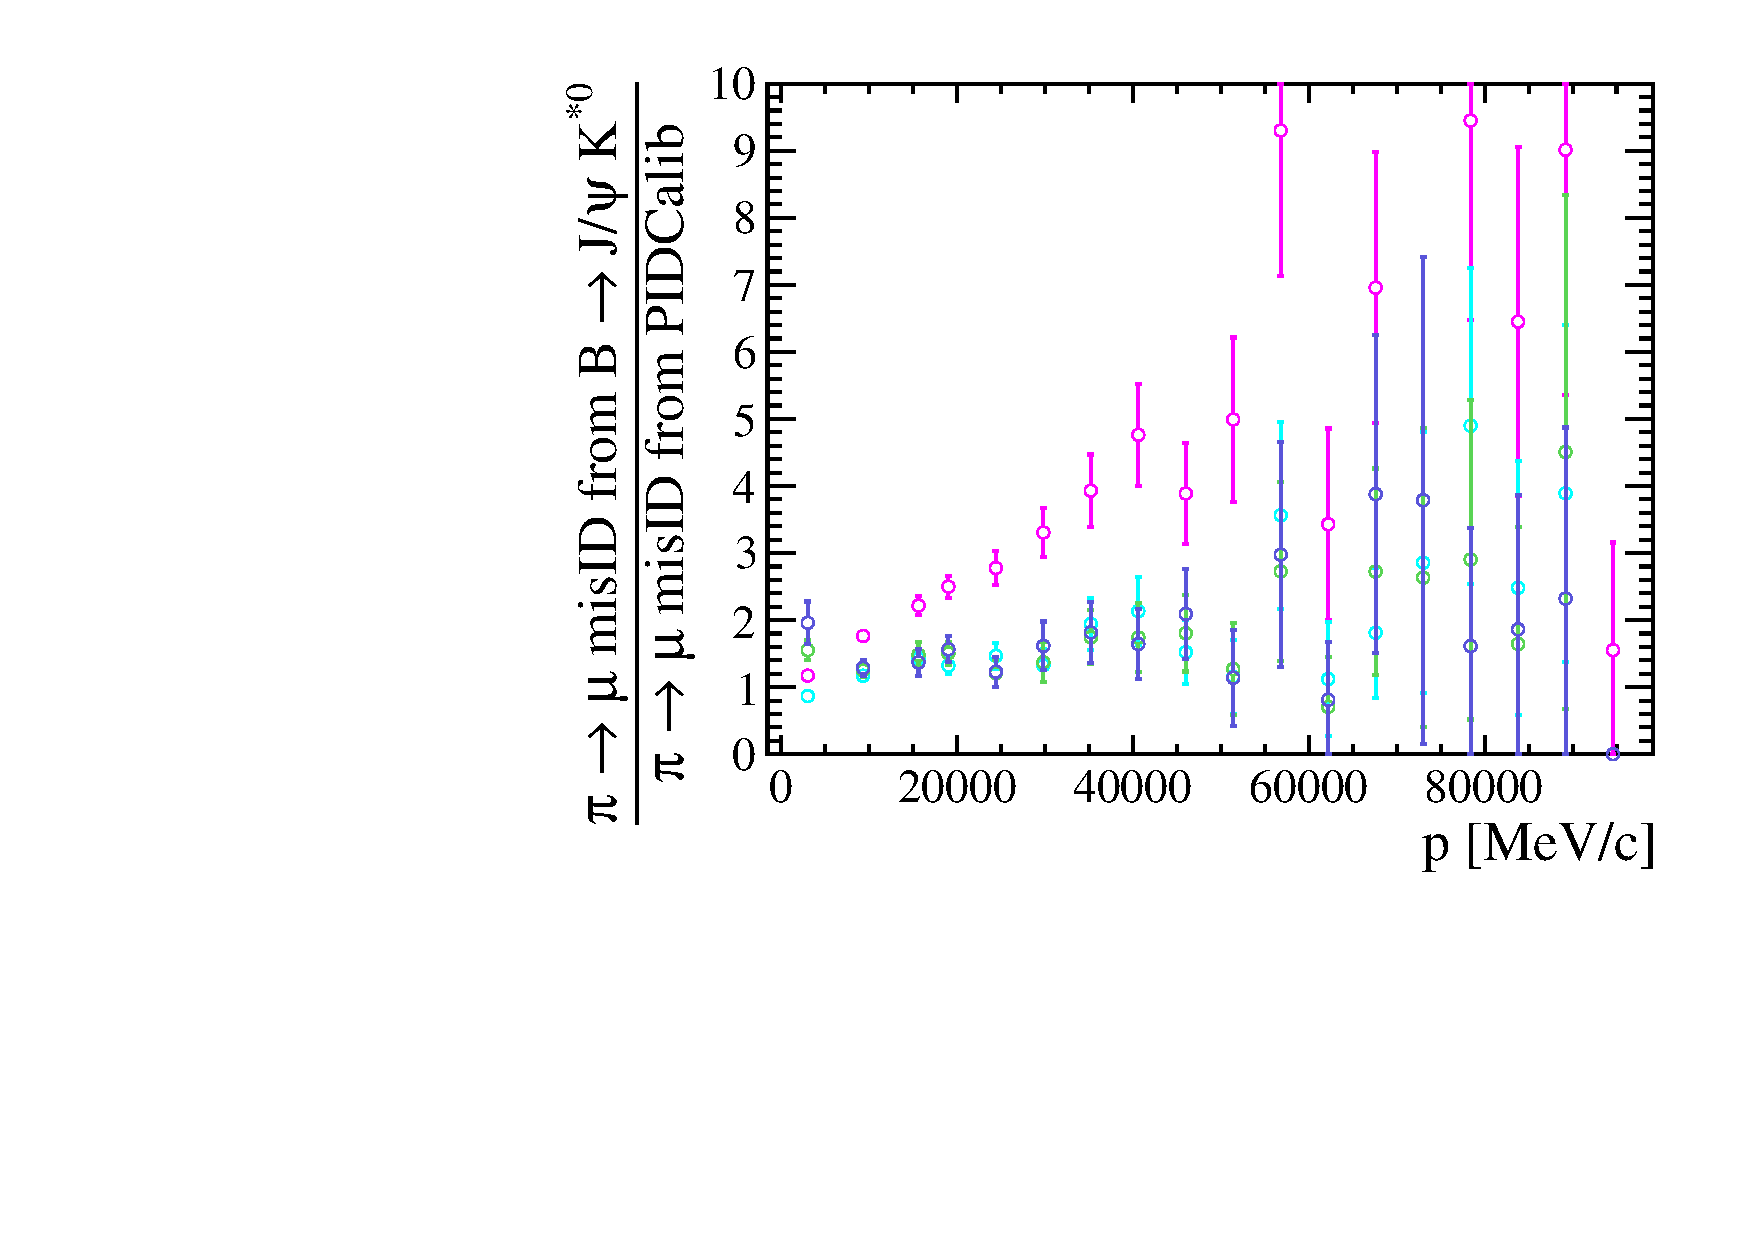
\includegraphics[width = 0.5\textwidth]{figs/trimuon/jpsikst/2012/Visualize_Ratios_PionMisid_small_thesis.pdf}\put(-50,133){(b)}
		\newline
%		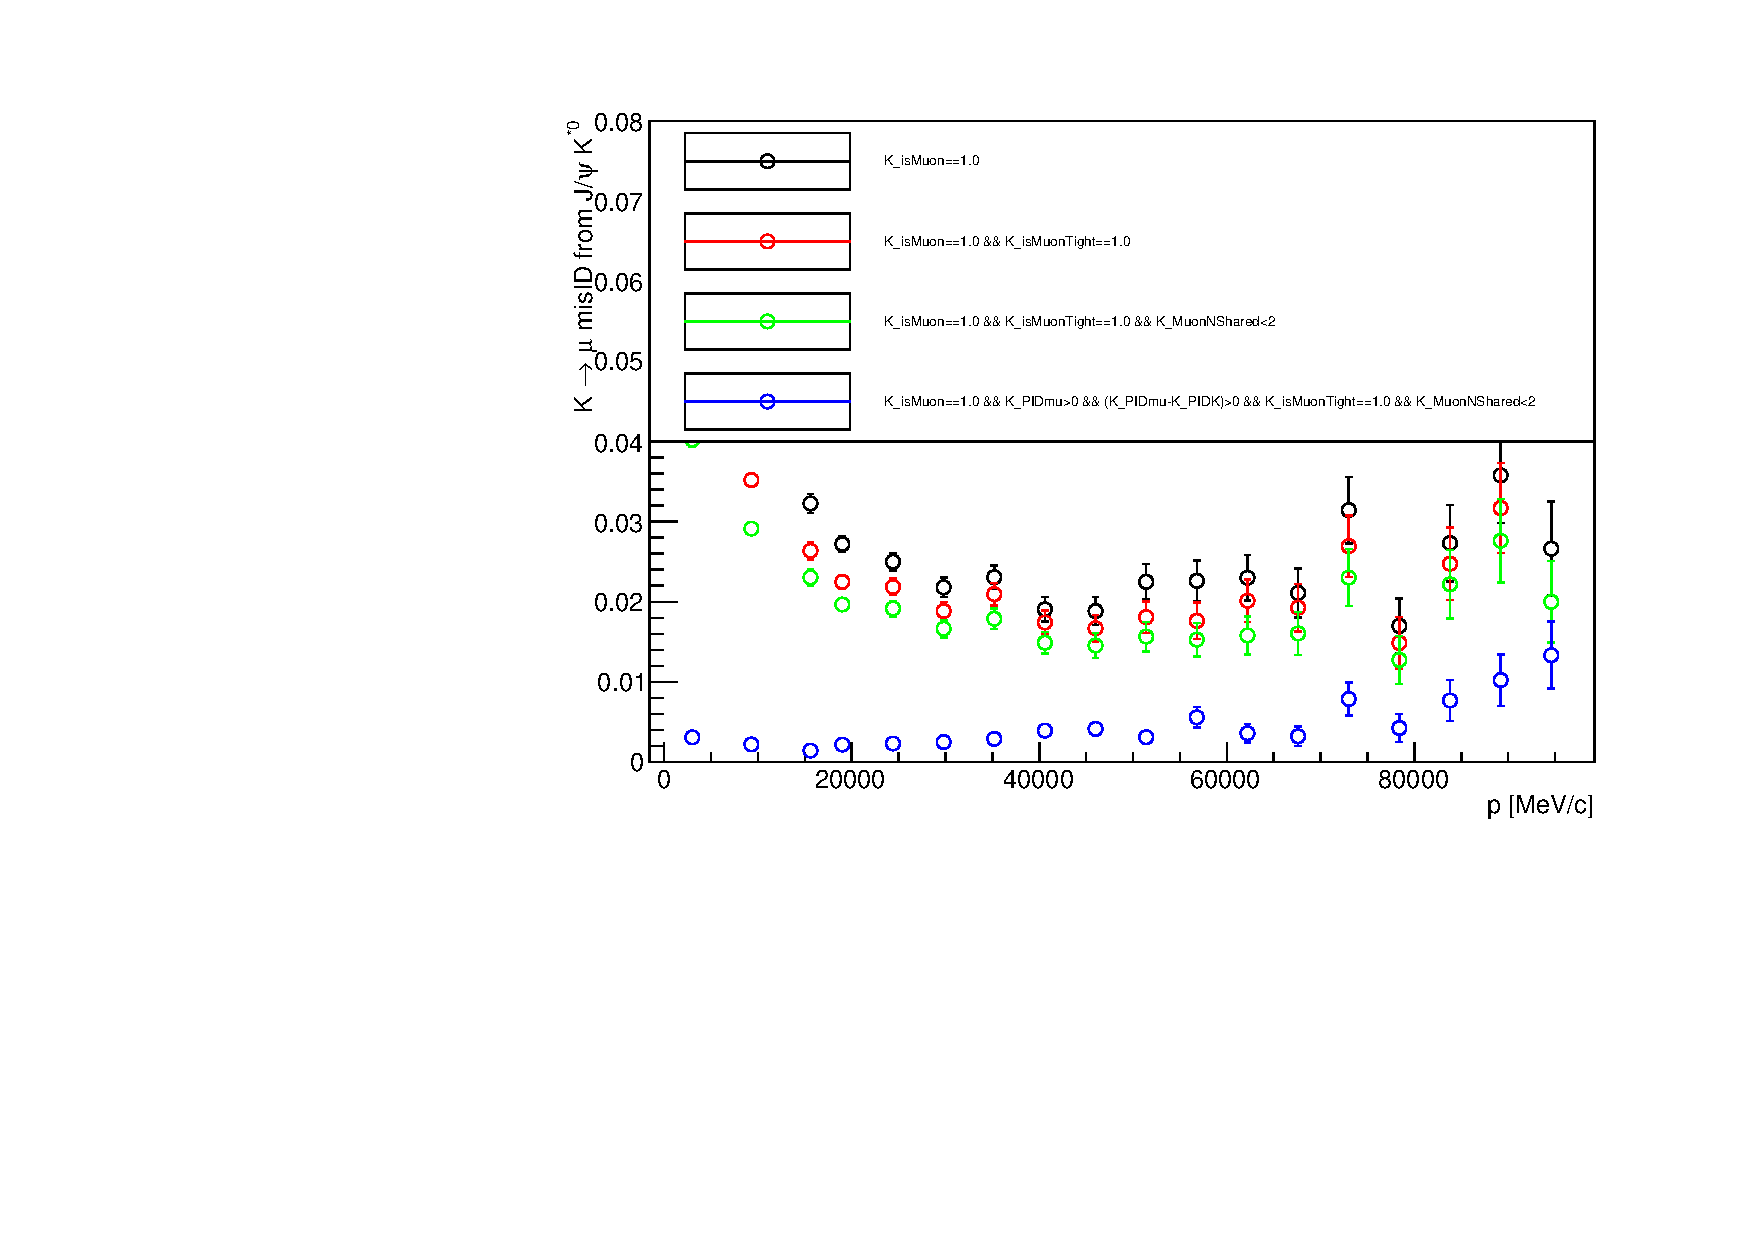
\includegraphics[width = 0.55\textwidth]{figs/trimuon/jpsikst/2012/Visualize_Weights_KaonMisid_2016_small.pdf}\put(-50,133){(e)}%
		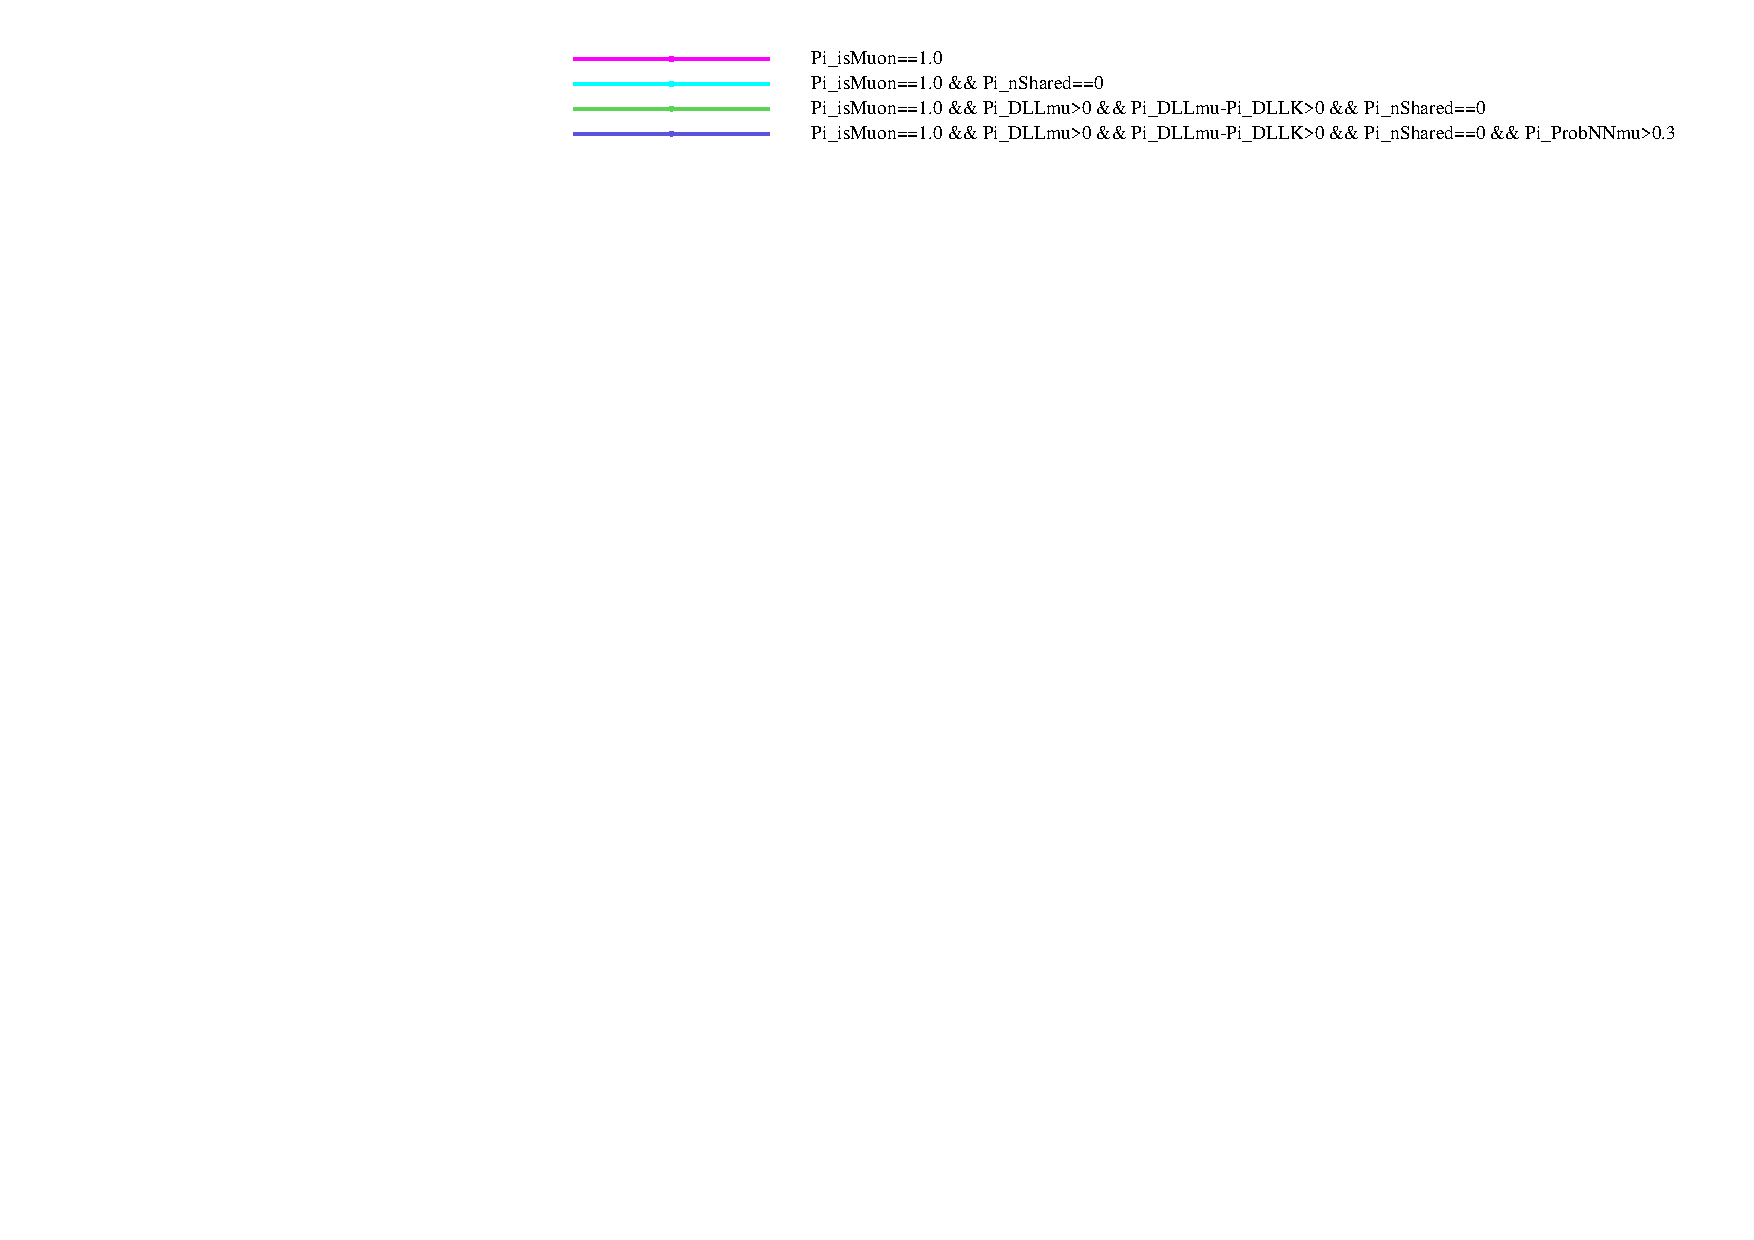
\includegraphics[width = 1.0\textwidth]{figs/trimuon/jpsikst/2012/Visualize_Weights_PionMisid_2012_small_thesis_legend.pdf}
		\caption{(a) $\pi \rightarrow \mu$ misID probabibility for different PID requirements obtained using $B^{0} \rightarrow J/\psi(\rightarrow \mu^{+} \mu^{-}) K^{*} (\rightarrow {K^{+} \pi^{-}} )$ for 2012 data. (b) This is compared to the standard \texttt{PIDCalib} $D^{*+}(\rightarrow D^{0}(\rightarrow K^{+} \pi^{-}) \pi^{+})$ sample. }
		\label{fig:JpsiKnew}
\end{figure}


In general the agreement is good in the low momenta regions between the two samples. These pions are softer and hence they will not be collimated, causing less interference with other two real muons in decay. However, in high momenta region, particles will tend to be more collimated. The influence of other two real muons in high momenta region will lead to bigger disagreement as these two real muons leave hits in the muon chambers with the collimated pion track, making the rate of \texttt{IsMuon==1.0} (pink) is higher. 

This disagreement is decreased by requiring \texttt{nShared==0.0} (blue), as having two other collimated muons to share hits will be more likely. The effect of other \gls{PID} variables can also be seen, but it is harder to interpret as these depend on several variables.

Even though this disagreement is decreased, it can be still noted that for the high momenta region $\pi \rightarrow \mu$ ~\autoref{fig:JpsiKnew} and $K \rightarrow \mu$ \autoref{fig:JpsiKaonnew} rate is 2 to 3 times higher with additional two real muon tracks, which is significant. 



\begin{figure}[h!]
\center
%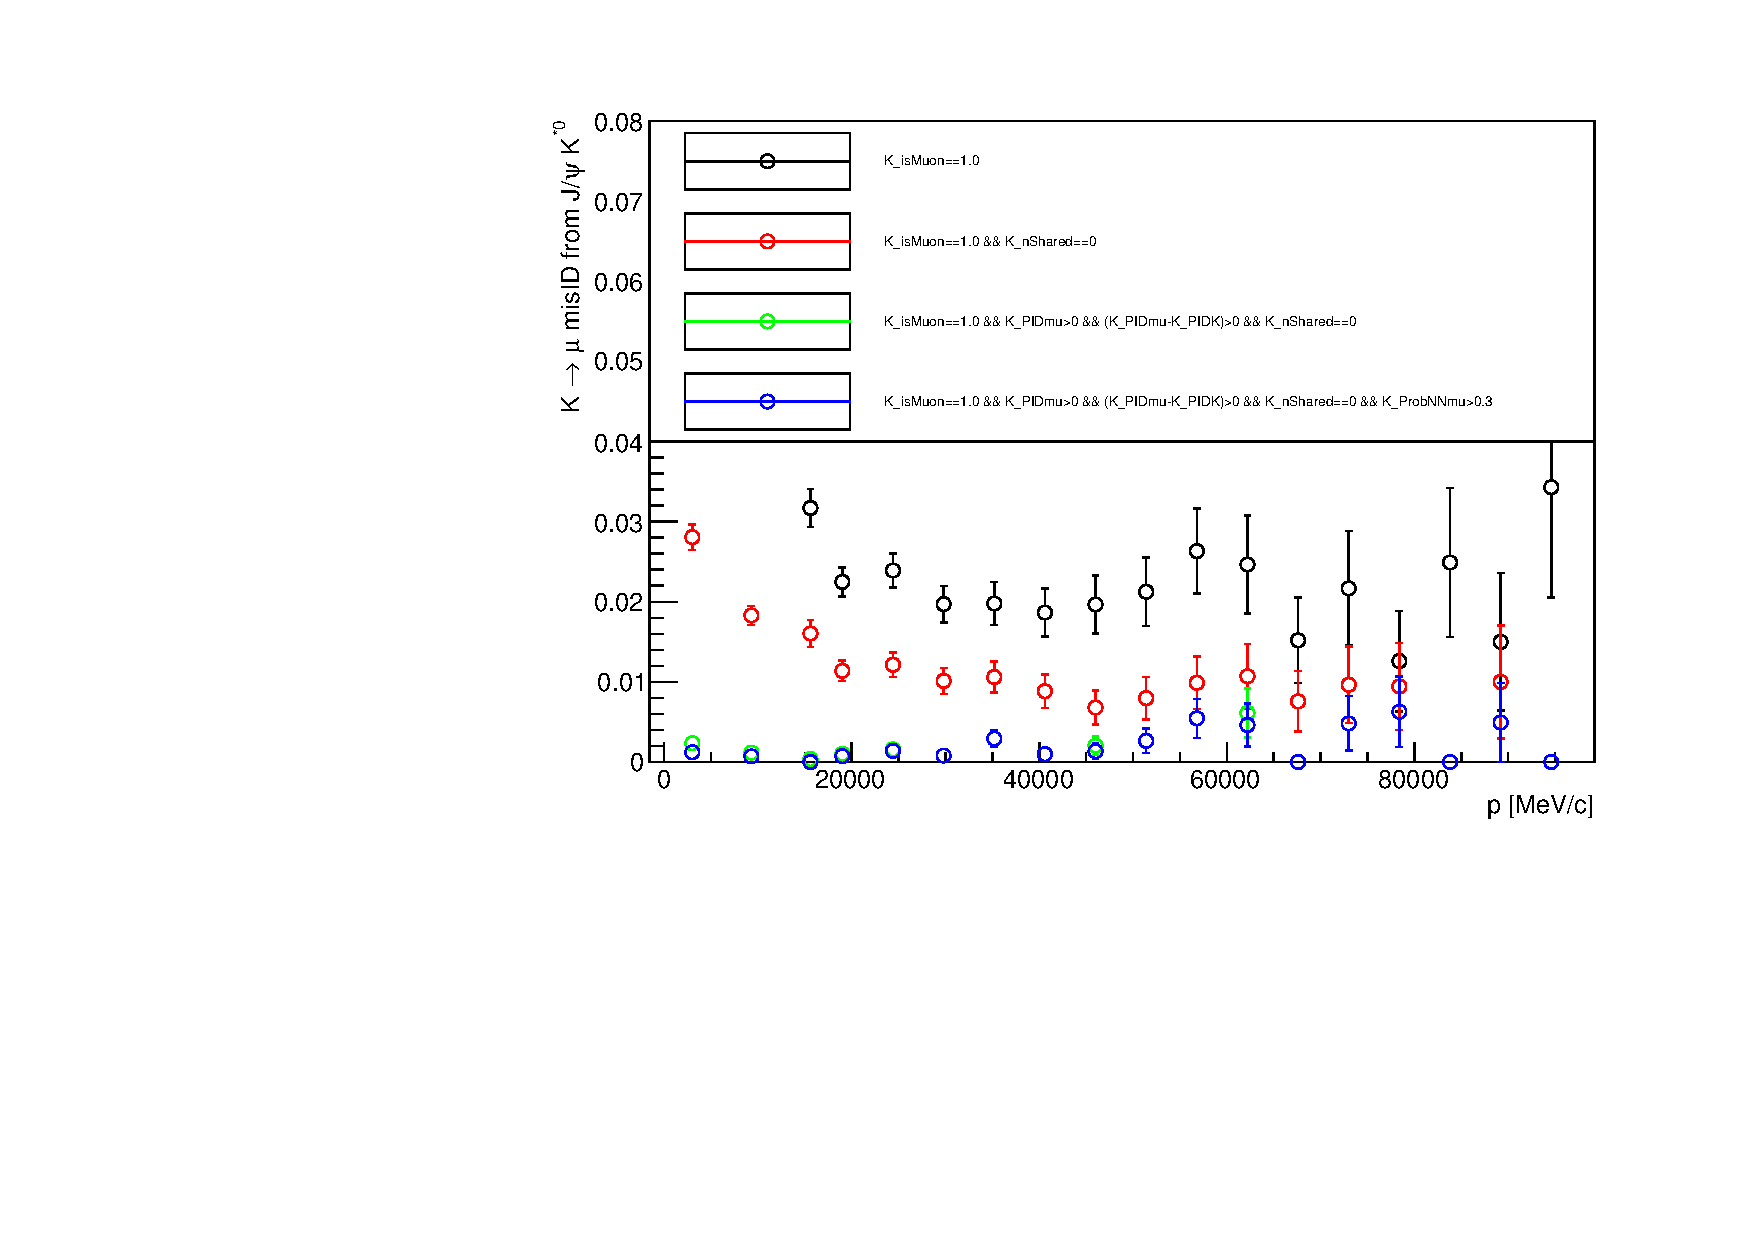
\includegraphics[width = 0.55\textwidth]{figs/trimuon/jpsikst/2012/Visualize_Weights_KaonMisid_2011_small.pdf}\put(-50,133){(a)}%
		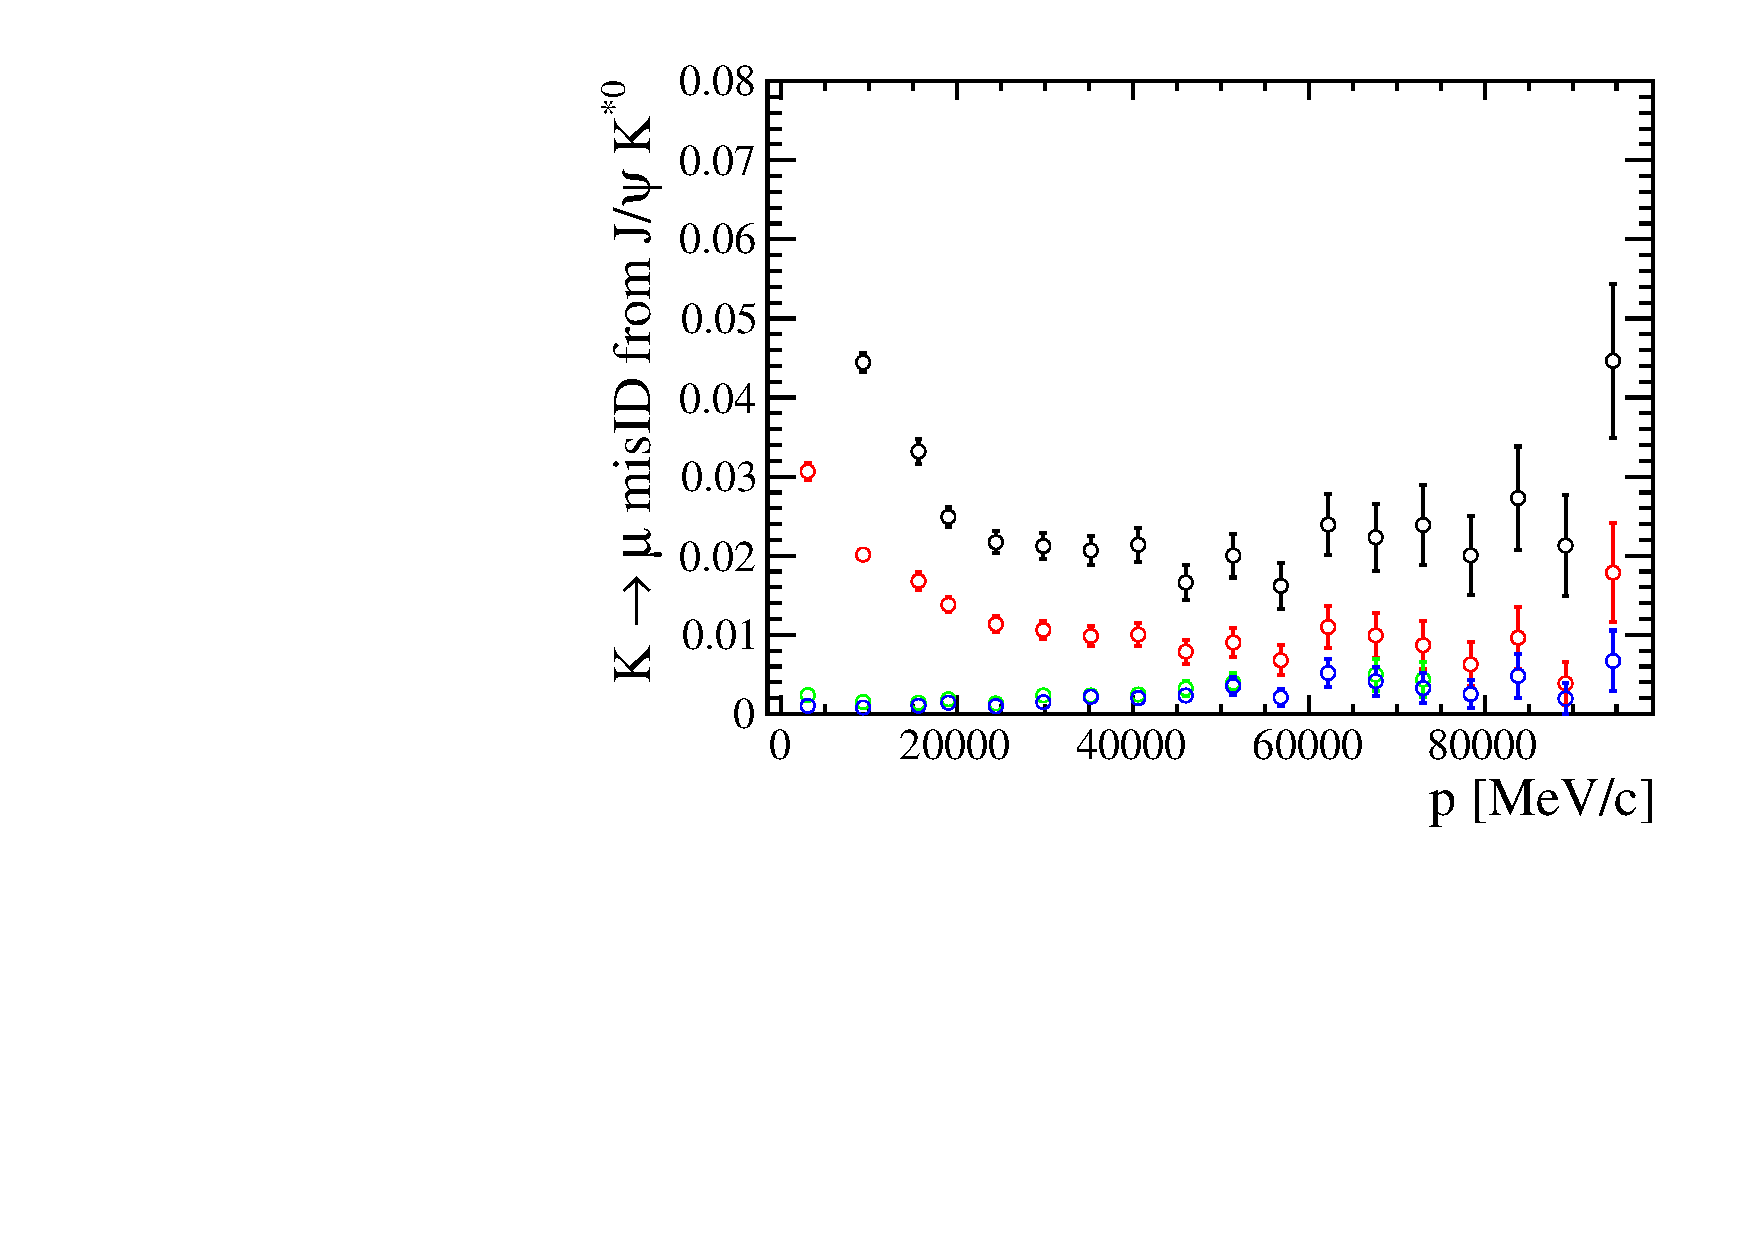
\includegraphics[width = 0.5\textwidth]{figs/trimuon/jpsikst/2012/Visualize_Weights_KaonMisid_2012_small_thesis.pdf}\put(-50,133){(a)}
%		\newline
%		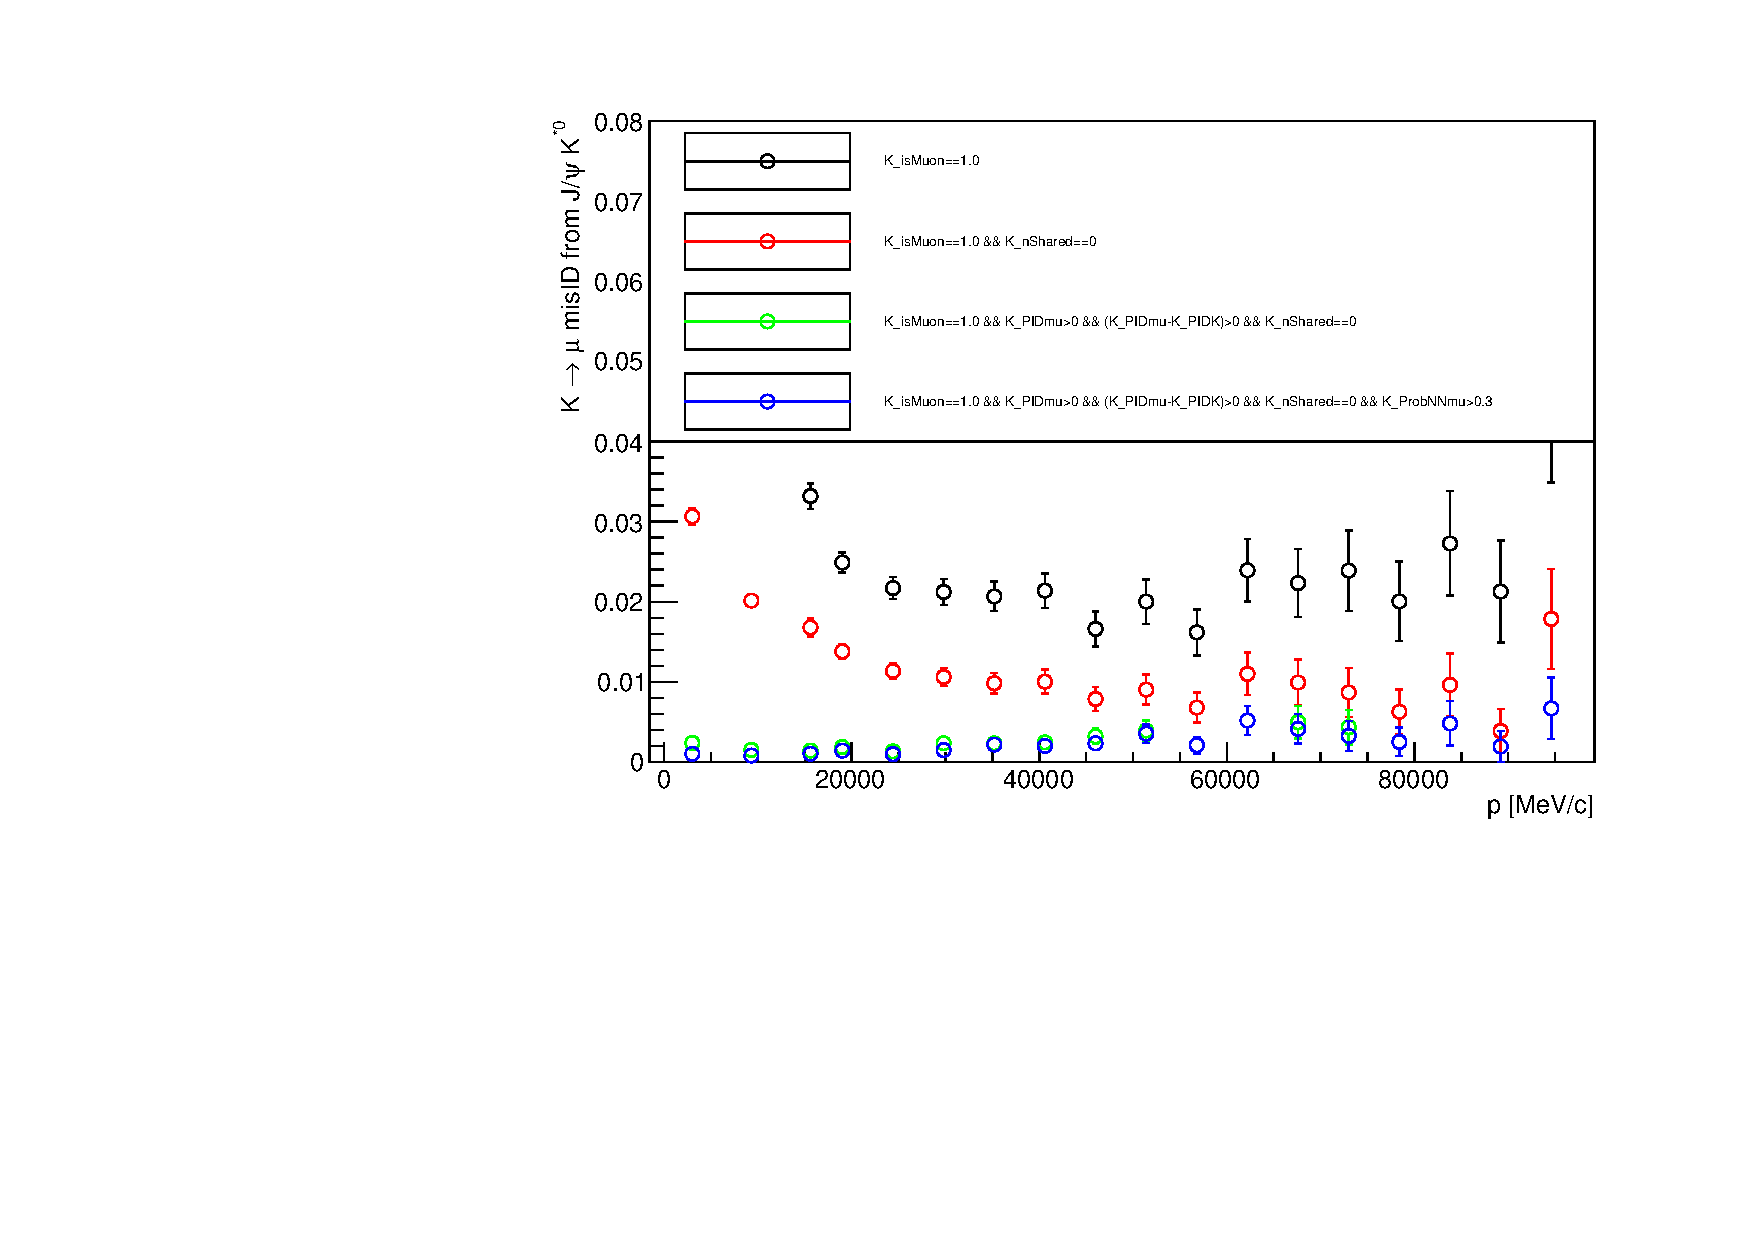
\includegraphics[width = 0.55\textwidth]{figs/trimuon/jpsikst/2012/Visualize_Weights_KaonMisid_small.pdf}\put(-50,133){(c)}%
		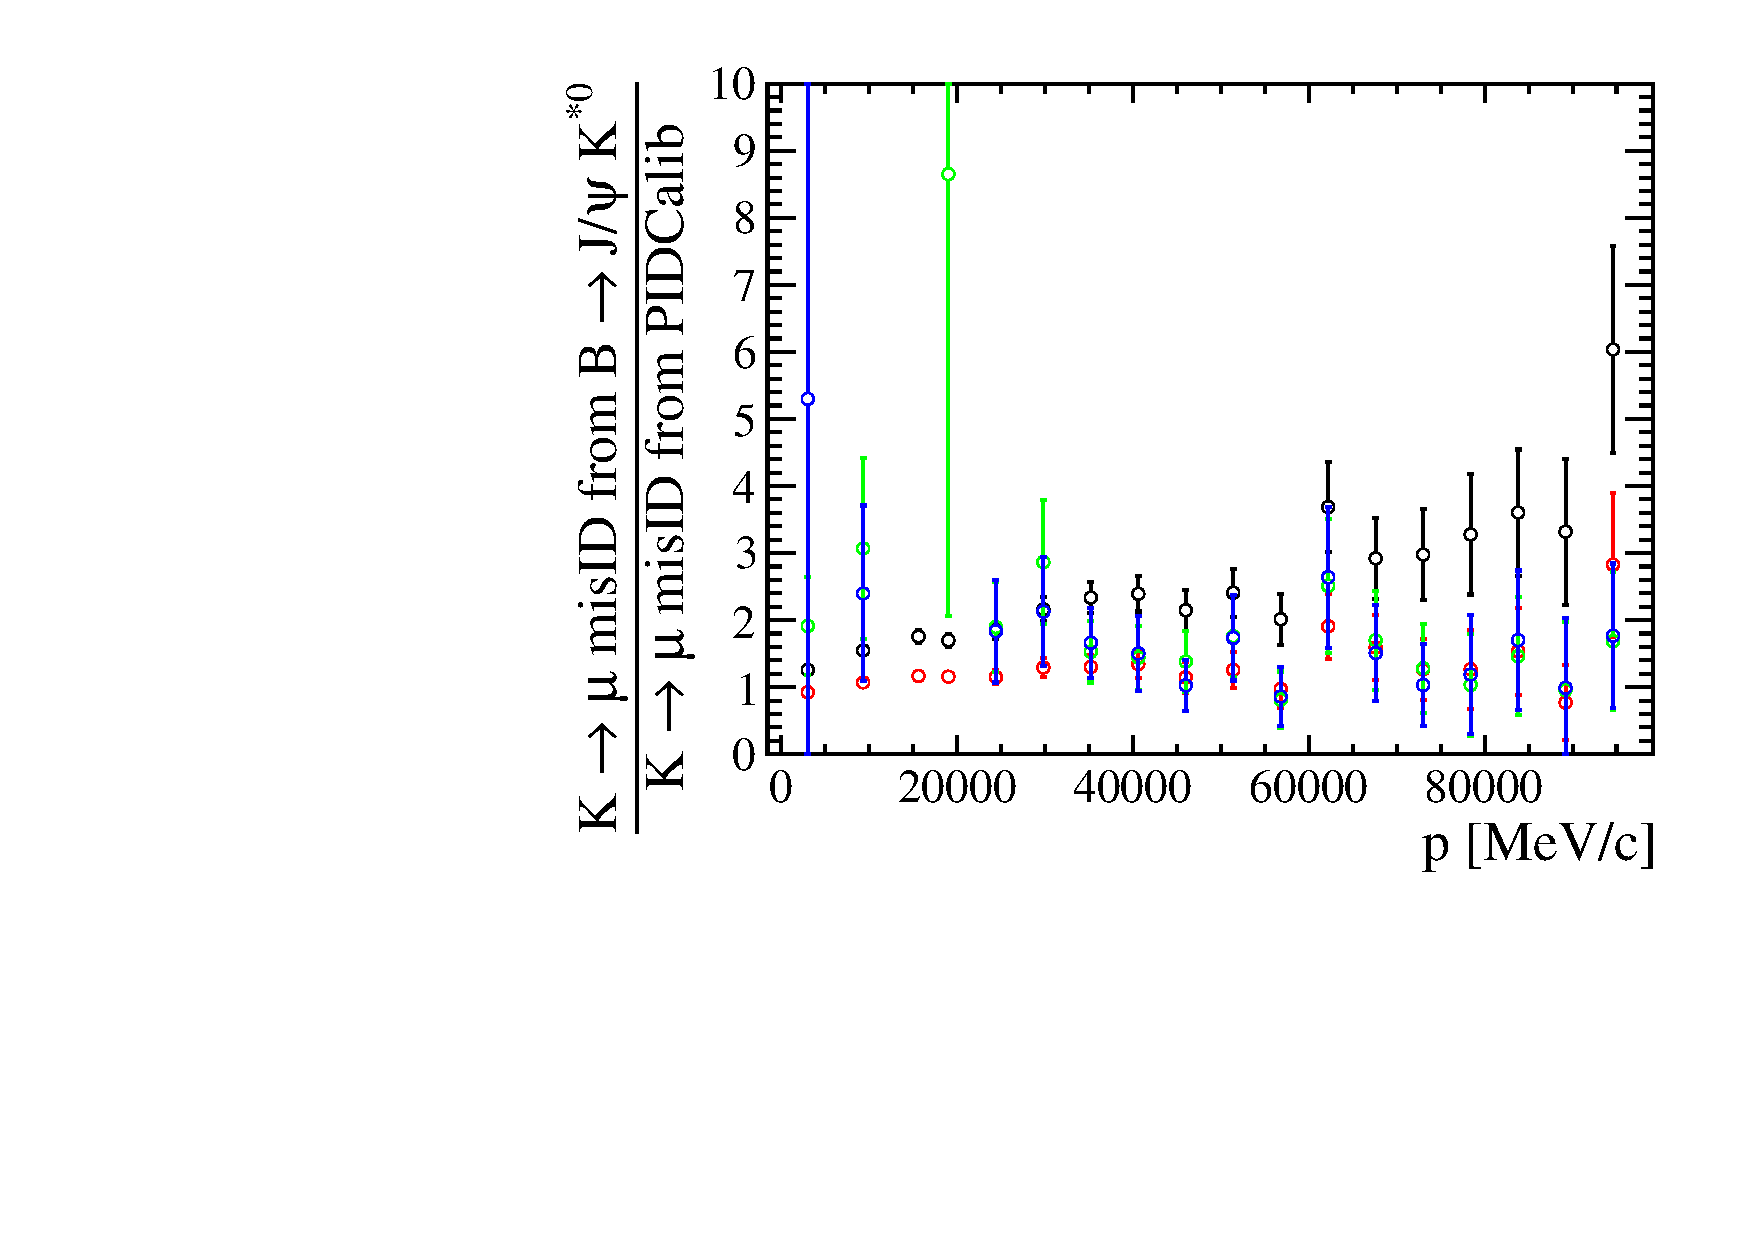
\includegraphics[width = 0.5\textwidth]{figs/trimuon/jpsikst/2012/Visualize_Ratios_KaonMisid_small_thesis.pdf}\put(-50,133){(b)}
		\newline
%		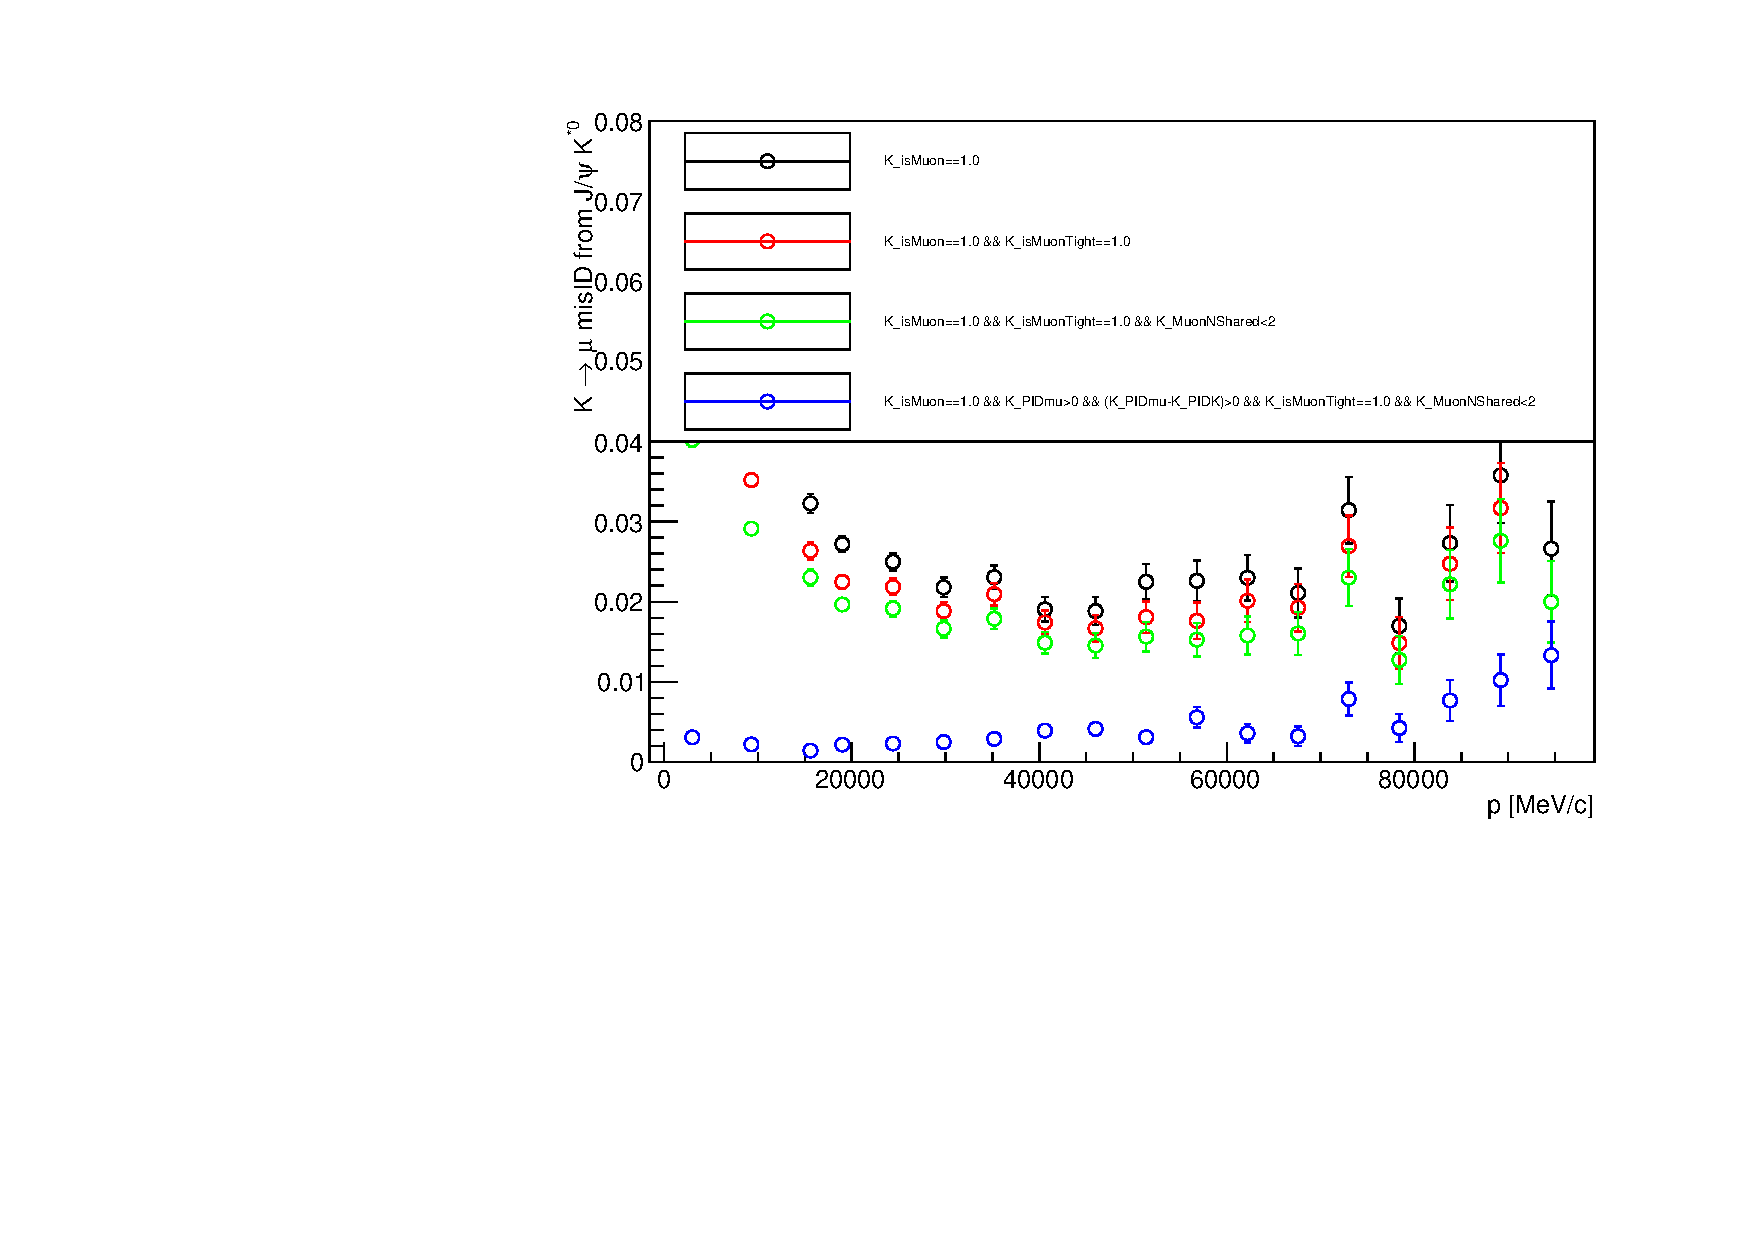
\includegraphics[width = 0.55\textwidth]{figs/trimuon/jpsikst/2012/Visualize_Weights_KaonMisid_2016_small.pdf}\put(-50,133){(e)}%
		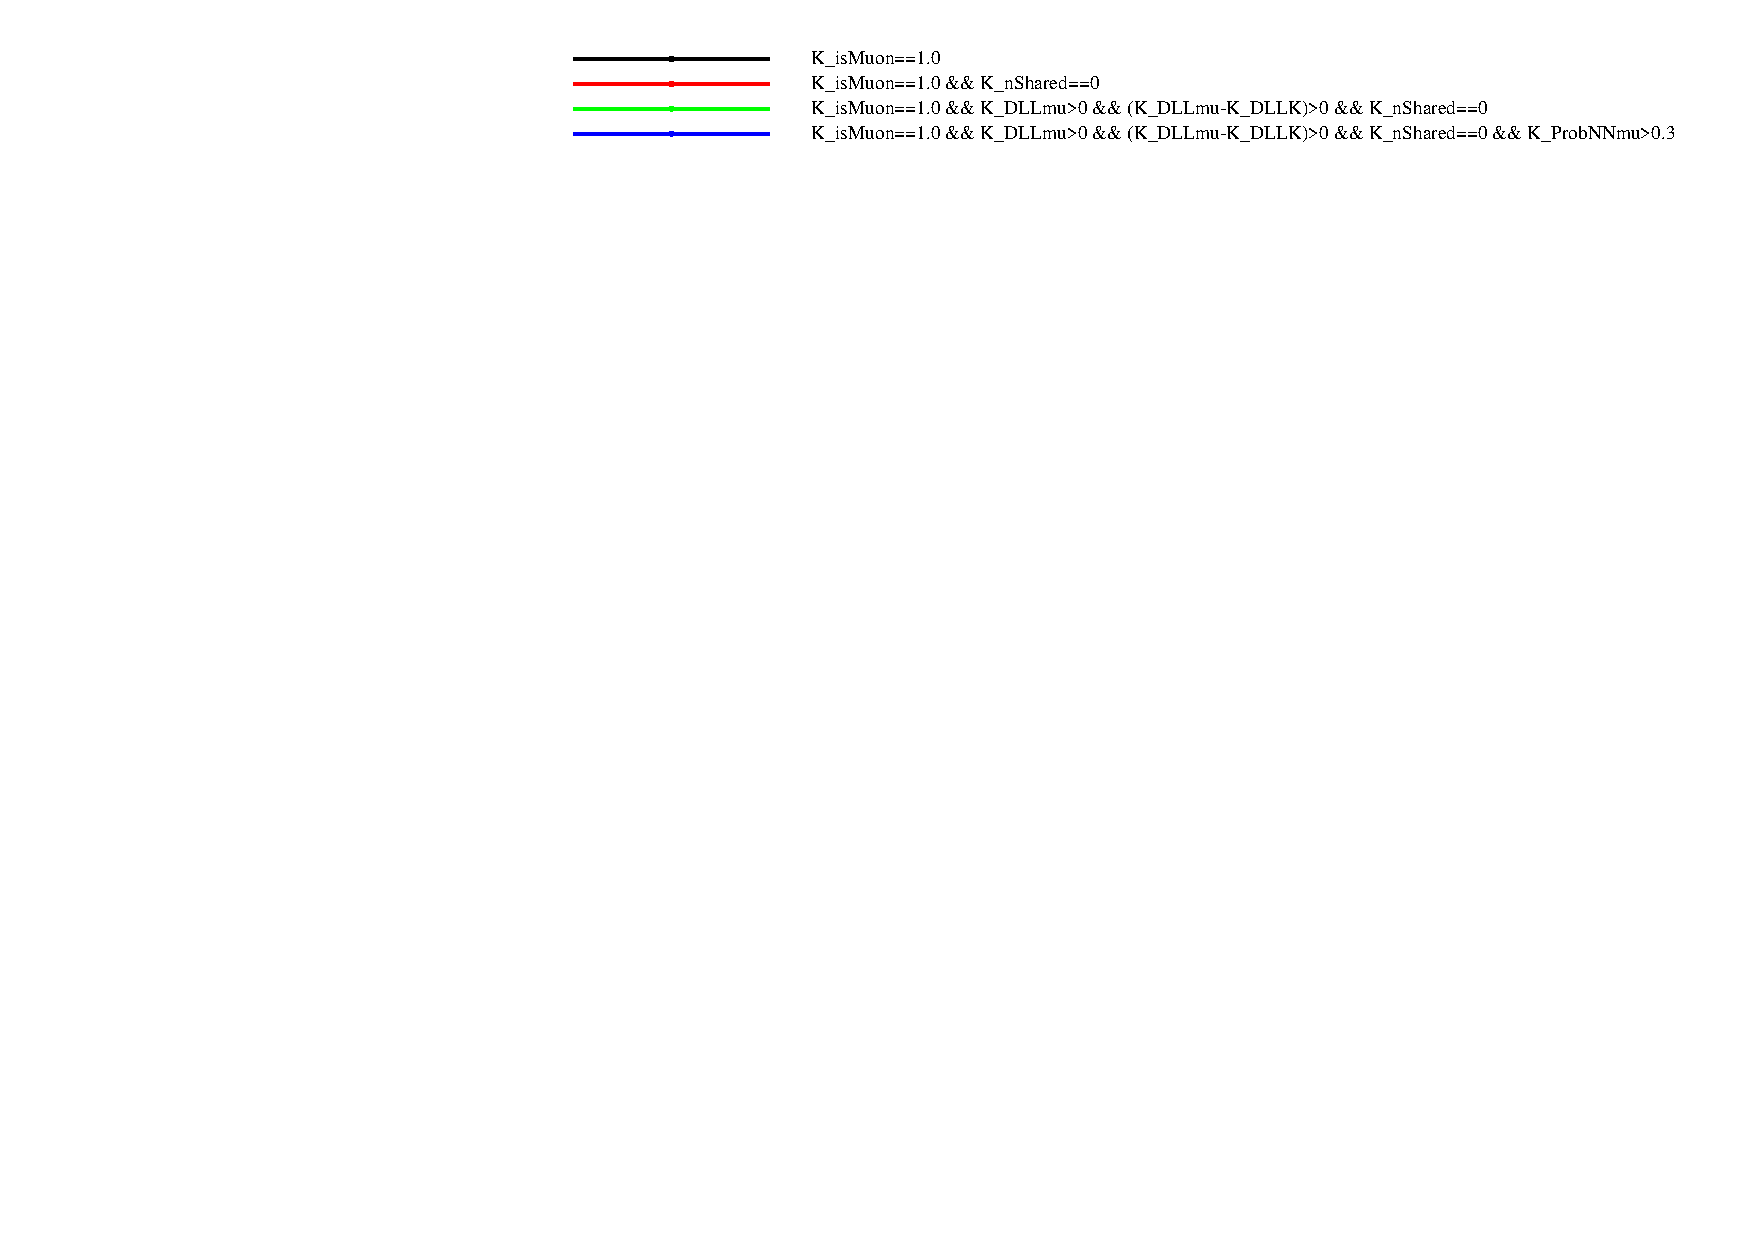
\includegraphics[width = 1.0\textwidth]{figs/trimuon/jpsikst/2012/Visualize_Weights_KaonMisid_2012_small_thesis_legend.pdf}
		\caption{(a) $K \rightarrow \mu$ misID probabibility for different PID requirements obtained using $B^{0} \rightarrow J/\psi(\rightarrow \mu^{+} \mu^{-}) K^{*} (\rightarrow {K^{+} \pi^{-}} )$ for 2012 data. (b) This is compared to the standard \texttt{PIDCalib} $D^{*+}(\rightarrow D^{0}(\rightarrow K^{+} \pi^{-}) \pi^{+})$ sample. }
		\label{fig:JpsiKaonnew}
\end{figure}

Due to the different \gls{PID} definitions of \texttt{nShared} between Run \Rn{1} and \Rn{2}, different \gls{PID} requirement are tested.  Results for $\pi \rightarrow \mu$ and $K \rightarrow \mu$ are summarized in \autoref{fig:JpsiPionnew2016} and
 \autoref{fig:JpsiKaonnew2016}. The misID probabilities in 2016 for also show the same momentum dependent trend as in 2012. 



\begin{figure}[h!]
\center
%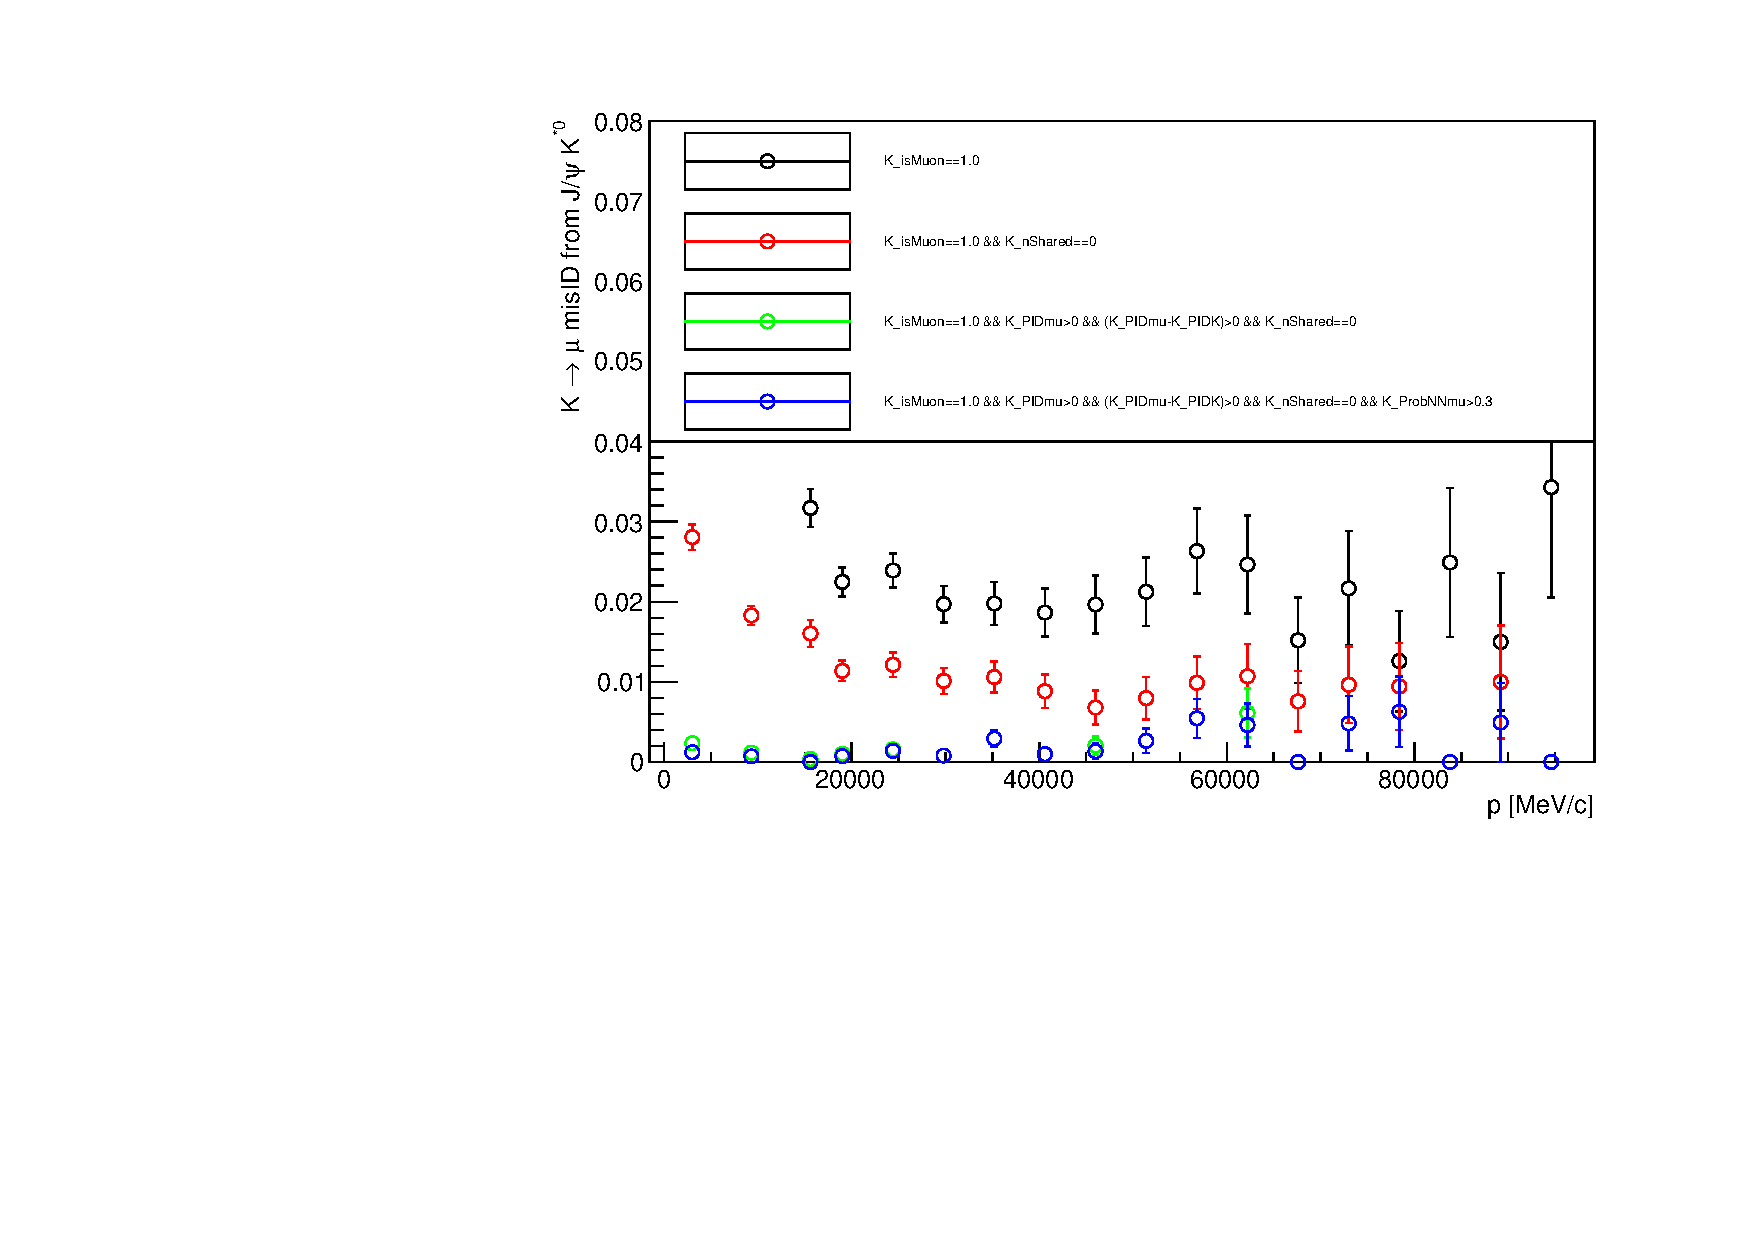
\includegraphics[width = 0.55\textwidth]{figs/trimuon/jpsikst/2012/Visualize_Weights_KaonMisid_2011_small.pdf}\put(-50,133){(a)}%
		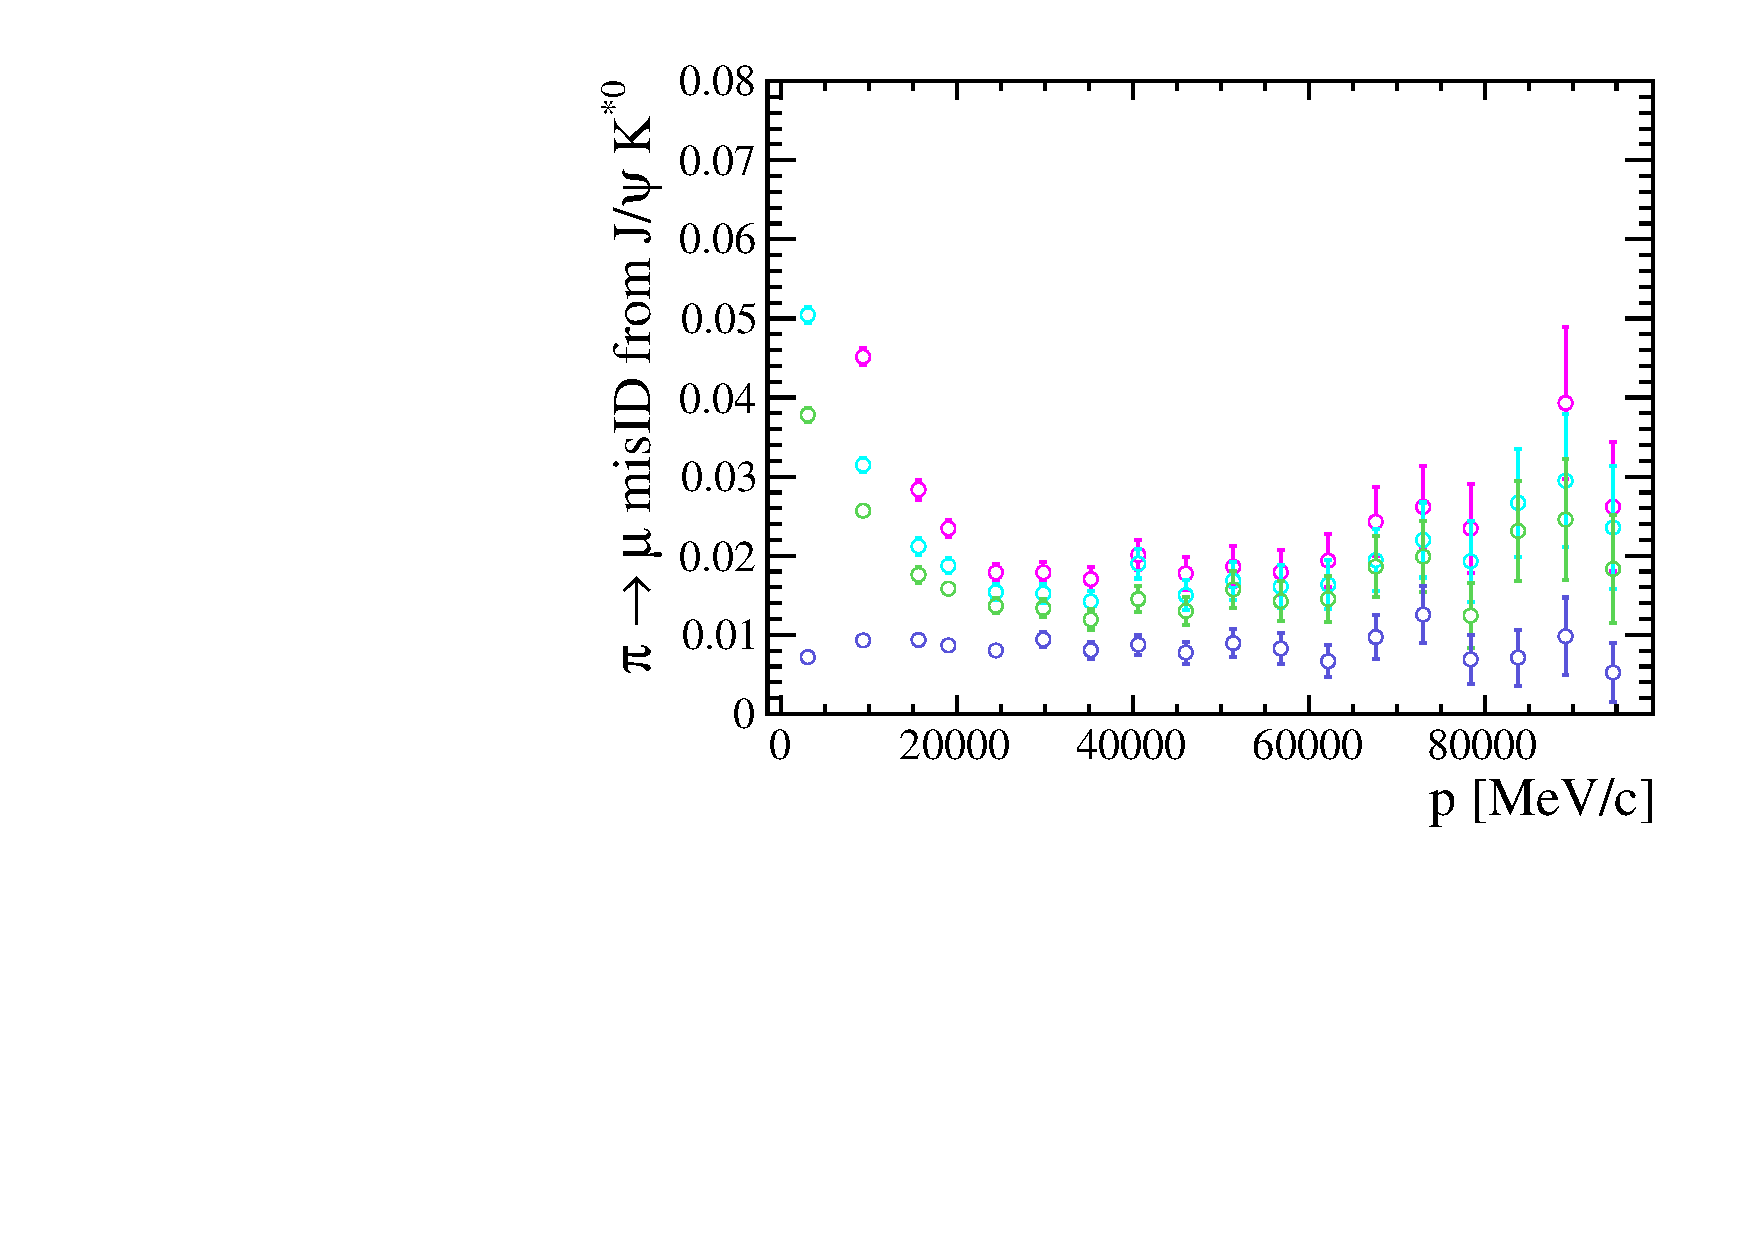
\includegraphics[width = 0.5\textwidth]{figs/trimuon/jpsikst/2016/Visualize_Weights_PionMisid_2016_small_thesis.pdf}\put(-50,133){(a)}
%		\newline
%		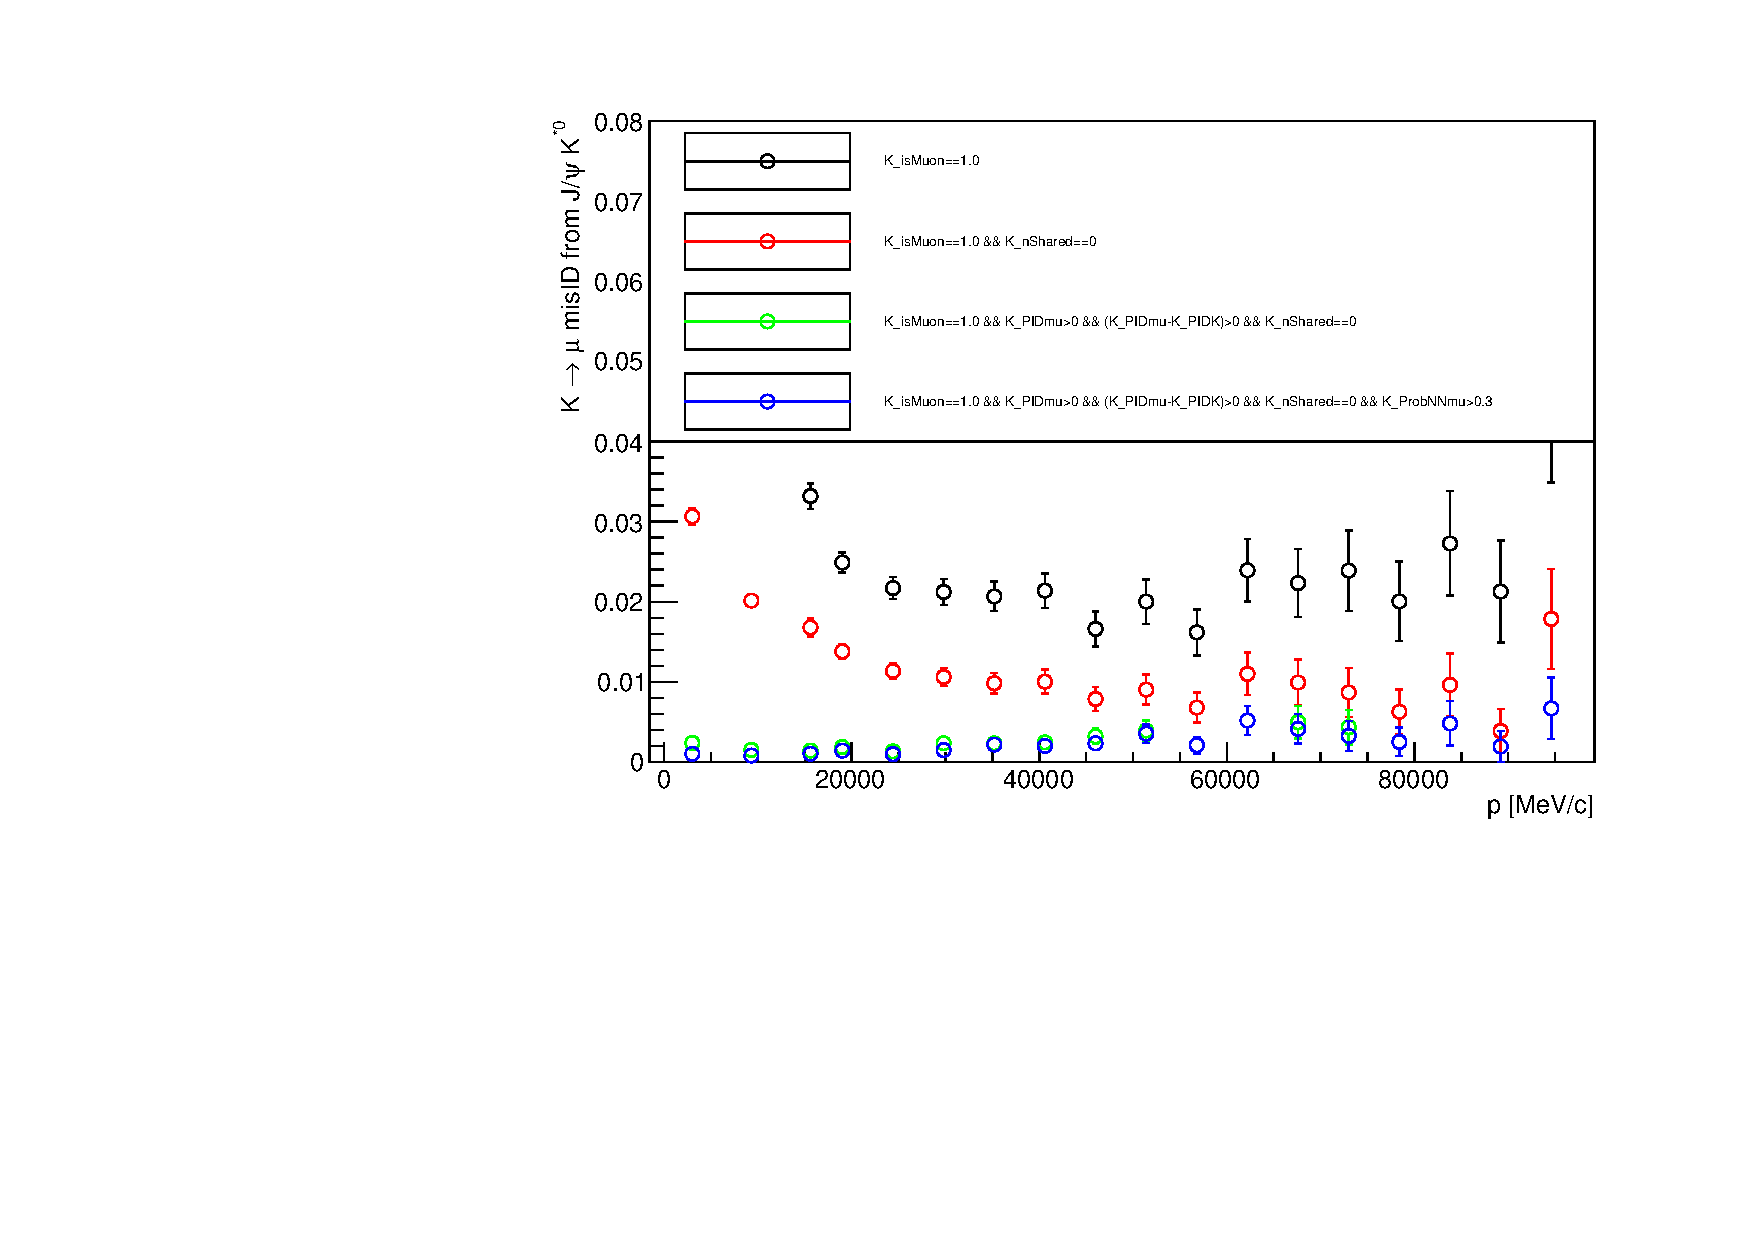
\includegraphics[width = 0.55\textwidth]{figs/trimuon/jpsikst/2012/Visualize_Weights_KaonMisid_small.pdf}\put(-50,133){(c)}%
		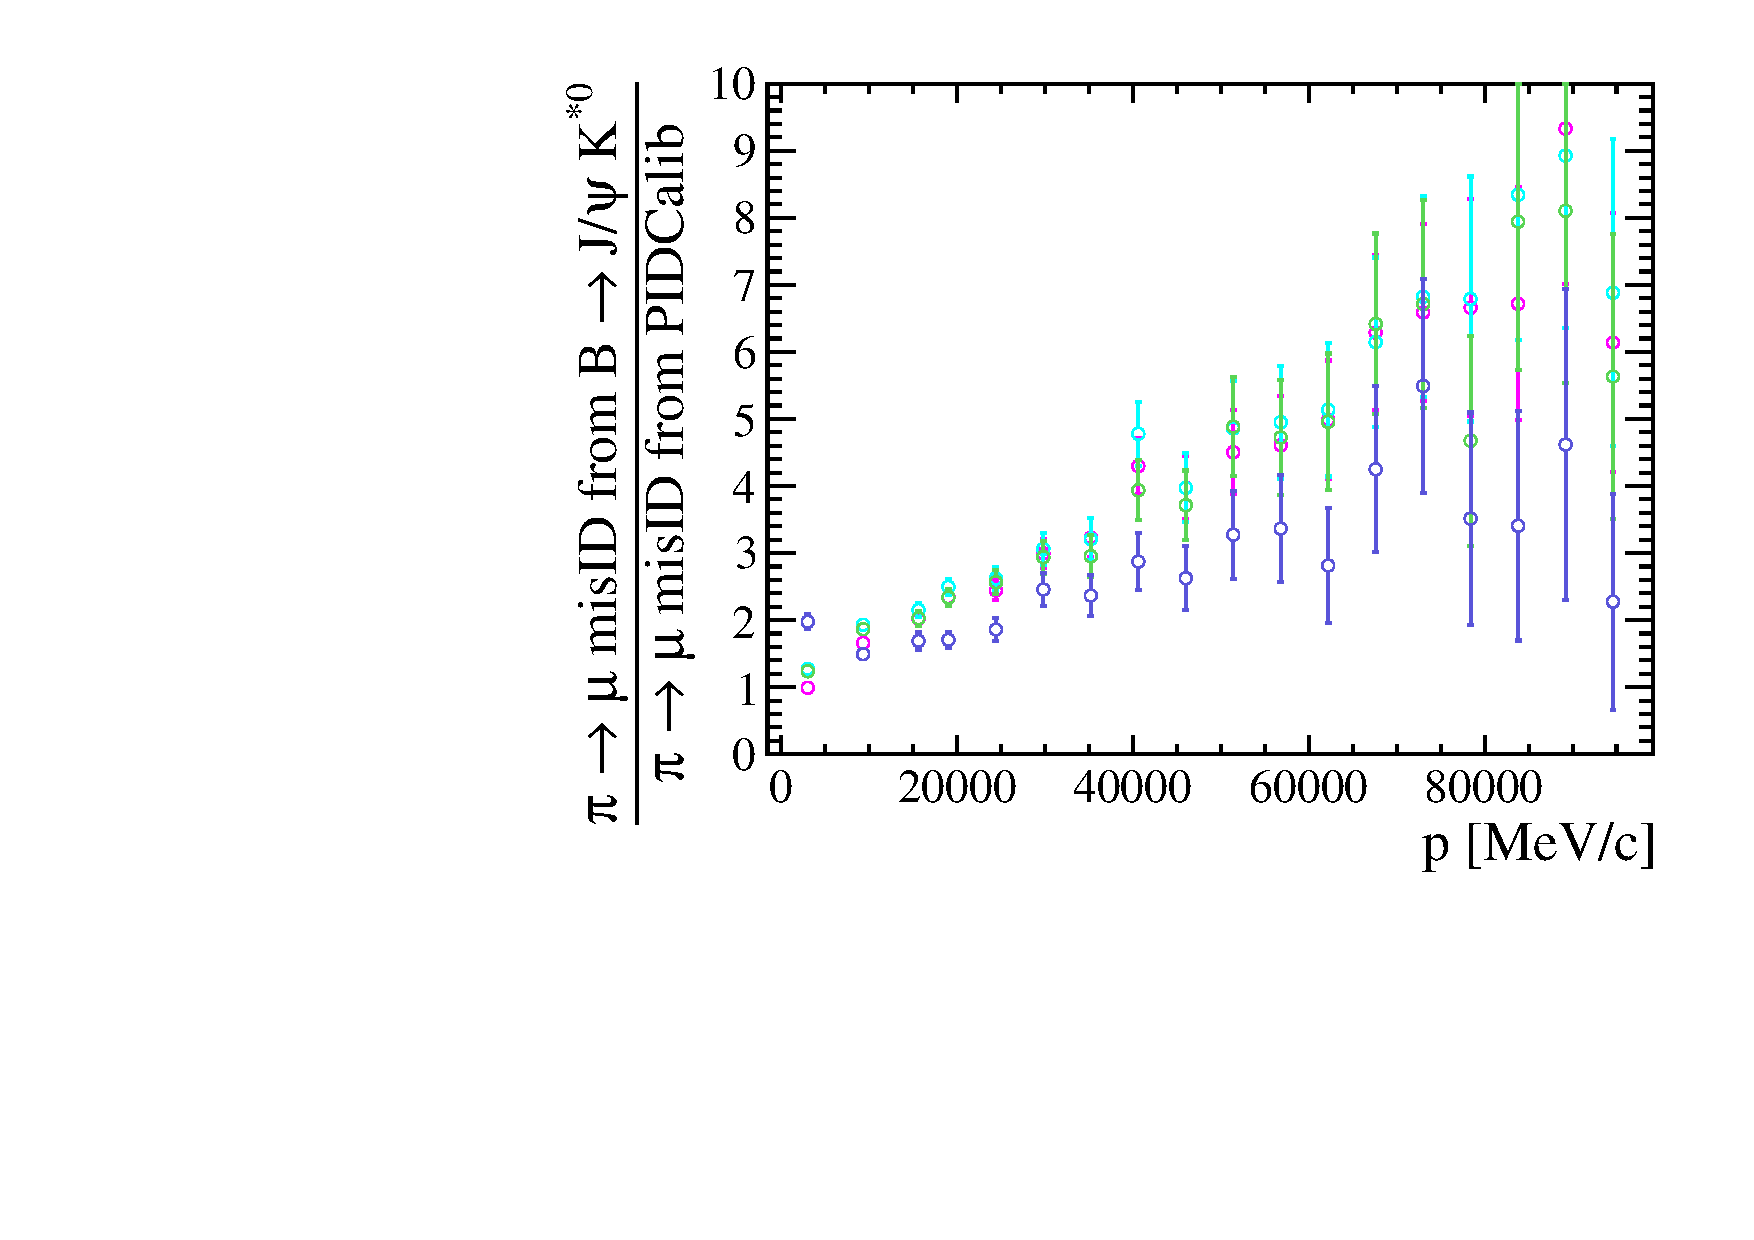
\includegraphics[width = 0.5\textwidth]{figs/trimuon/jpsikst/2016/Visualize_Ratios_PionMisid_2016_small_thesis.pdf}\put(-50,133){(b)}
		\newline
%		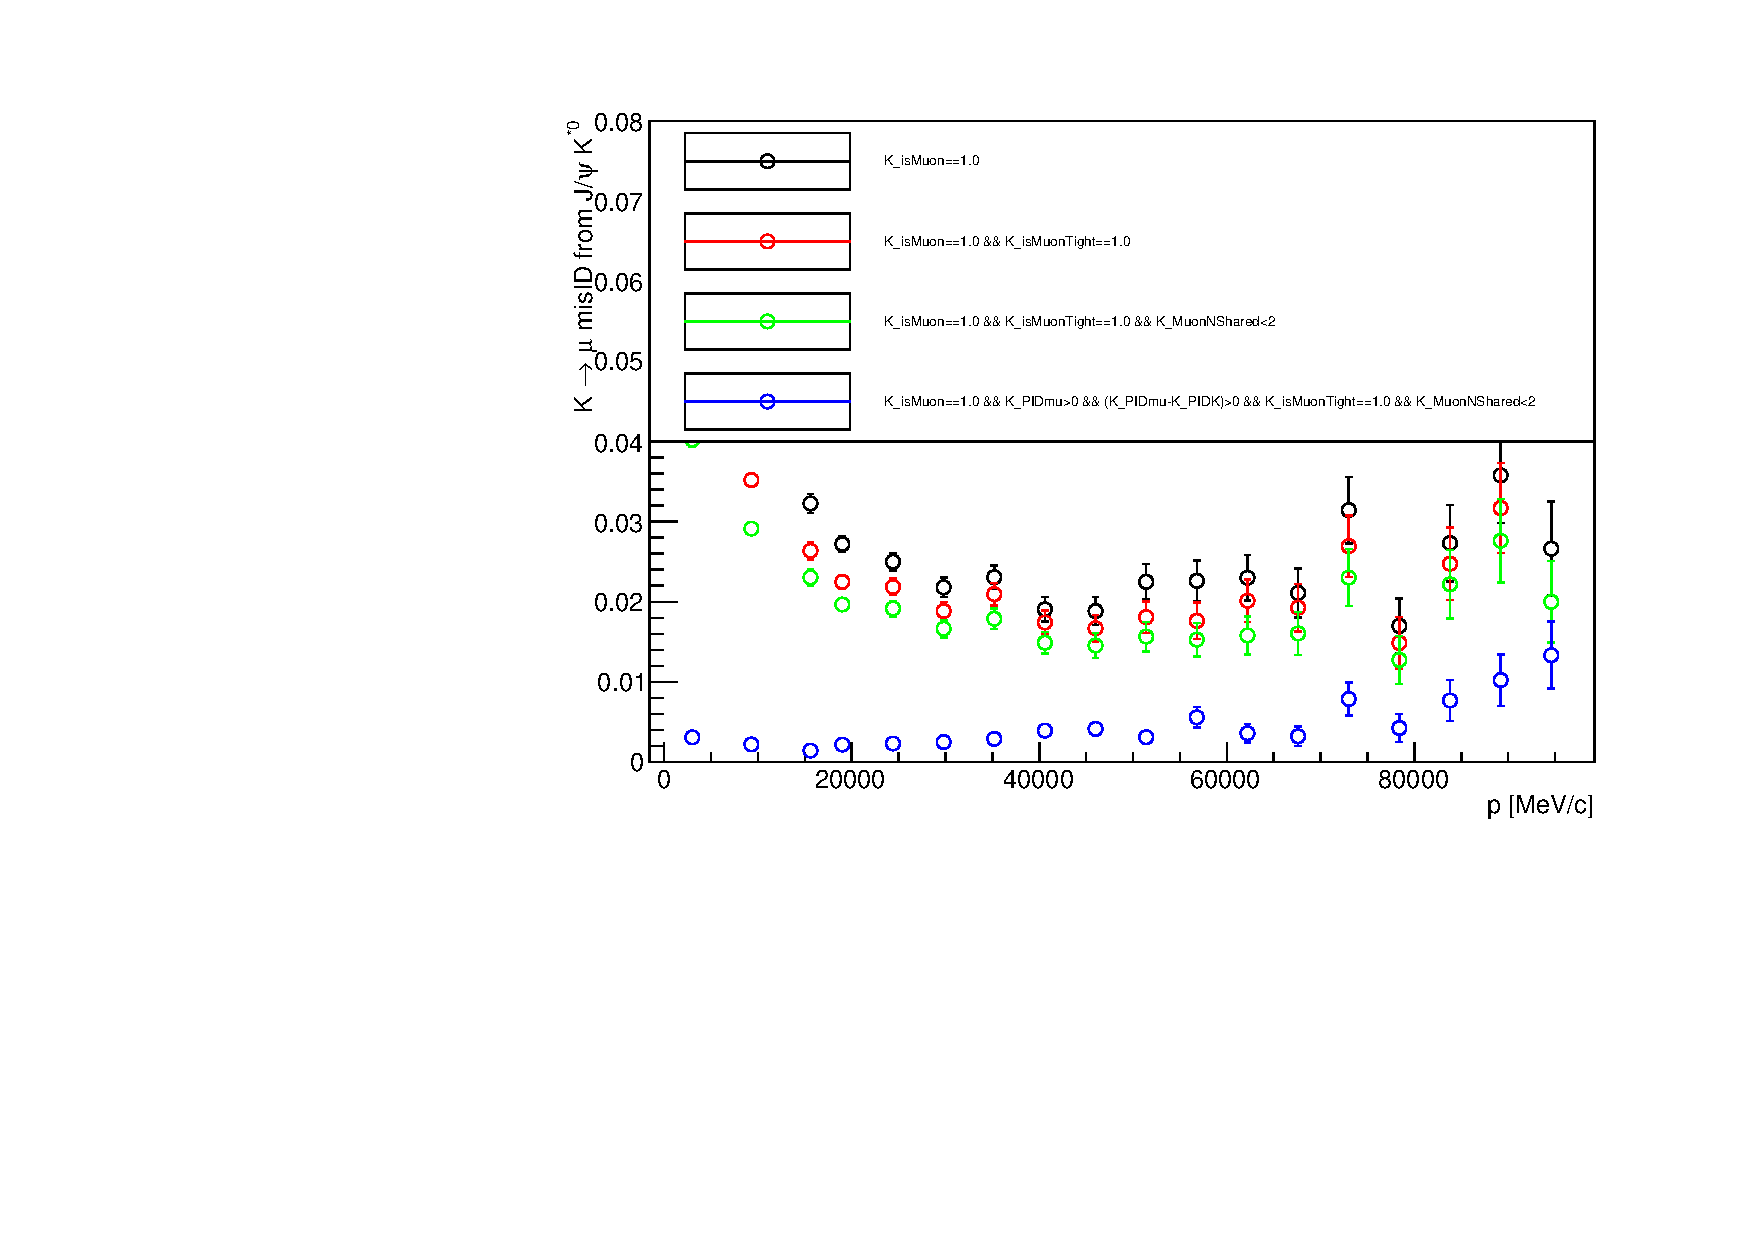
\includegraphics[width = 0.55\textwidth]{figs/trimuon/jpsikst/2012/Visualize_Weights_KaonMisid_2016_small.pdf}\put(-50,133){(e)}%
		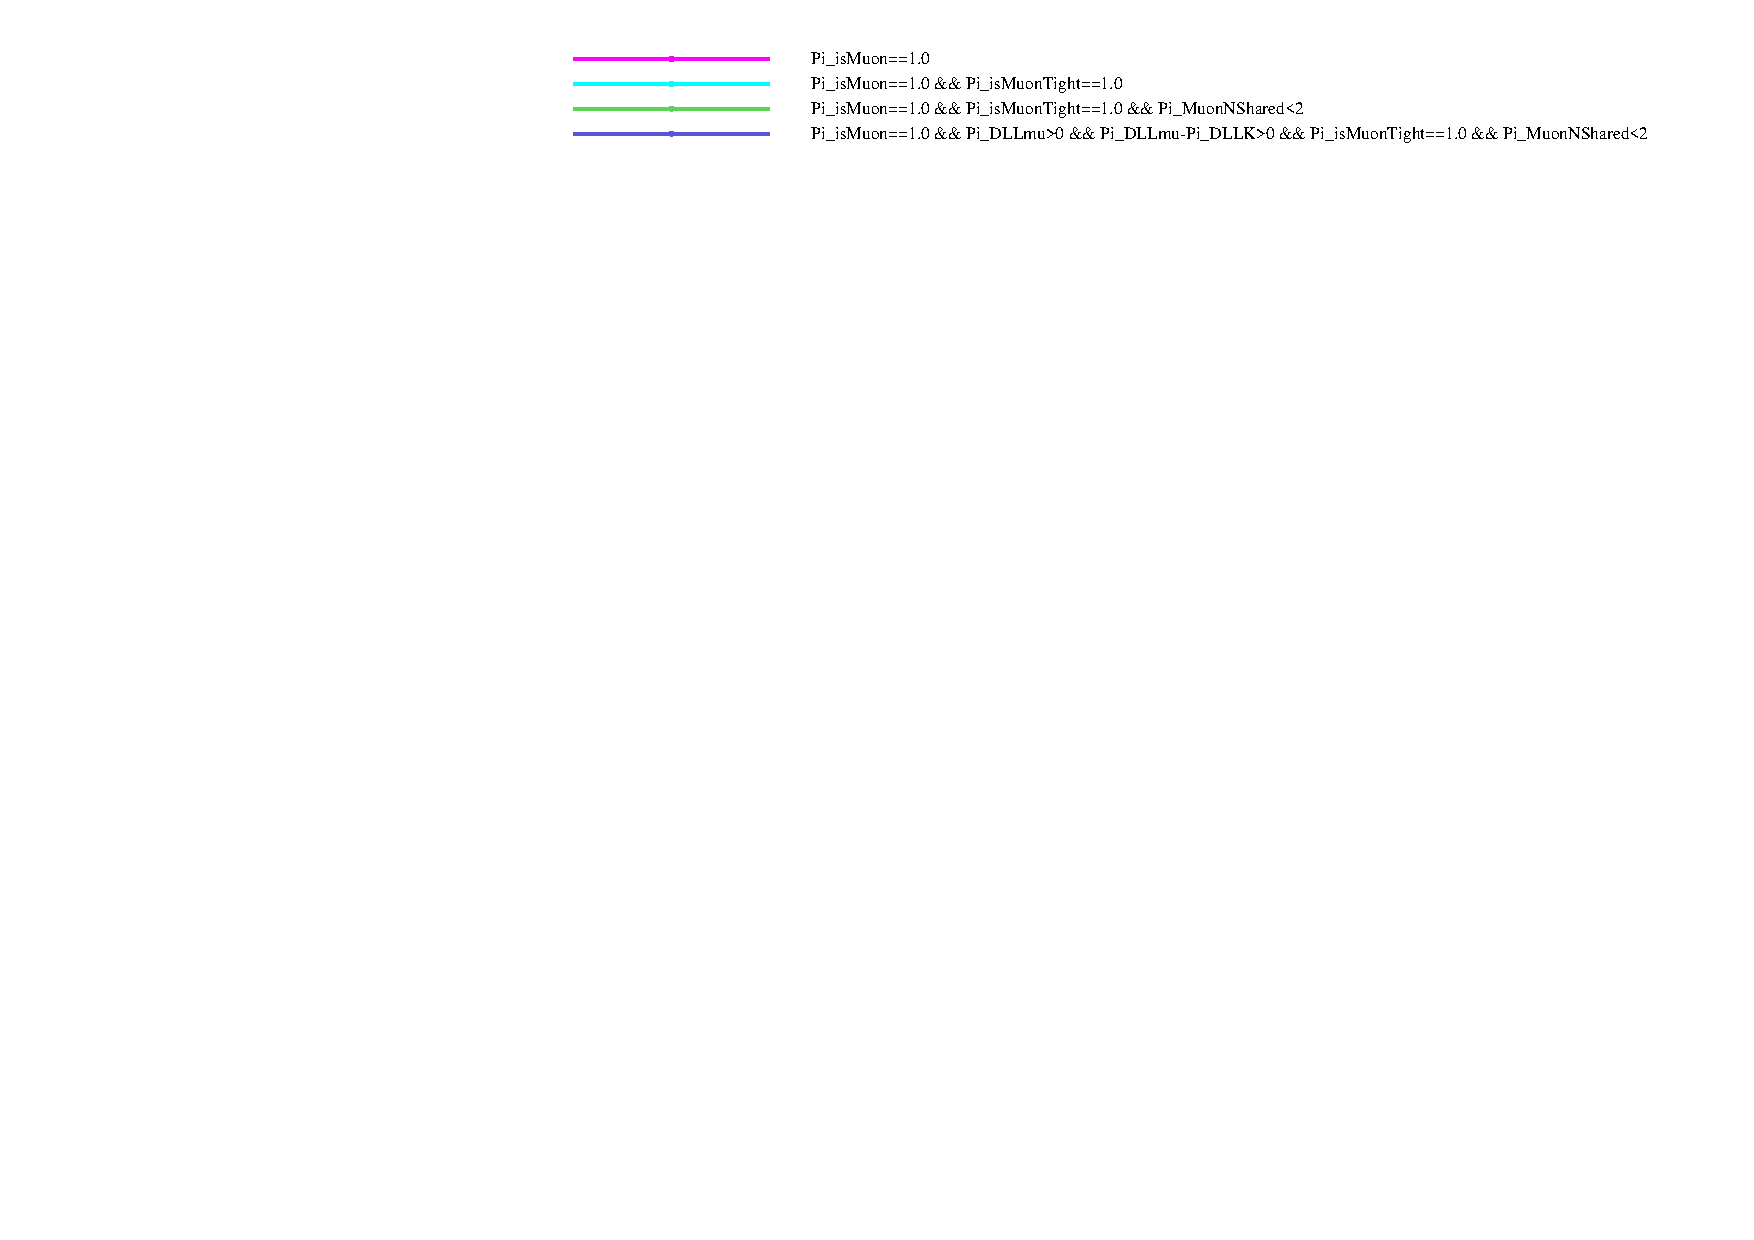
\includegraphics[width = 1.0\textwidth]{figs/trimuon/jpsikst/2016/Visualize_Weights_PionMisid_2016_small_thesis_legend.pdf}
		\caption{(a) $\pi \rightarrow \mu$ misID probabibility for different PID requirements obtained using $B^{0} \rightarrow J/\psi(\rightarrow \mu^{+} \mu^{-}) K^{*} (\rightarrow {K^{+} \pi^{-}} )$ for 2016 data. (b) This is compared to the standard \texttt{PIDCalib} $D^{*+}(\rightarrow D^{0}(\rightarrow K^{+} \pi^{-}) \pi^{+})$ sample. }
		\label{fig:JpsiPionnew2016}
\end{figure}


\begin{figure}[h!]
\center
%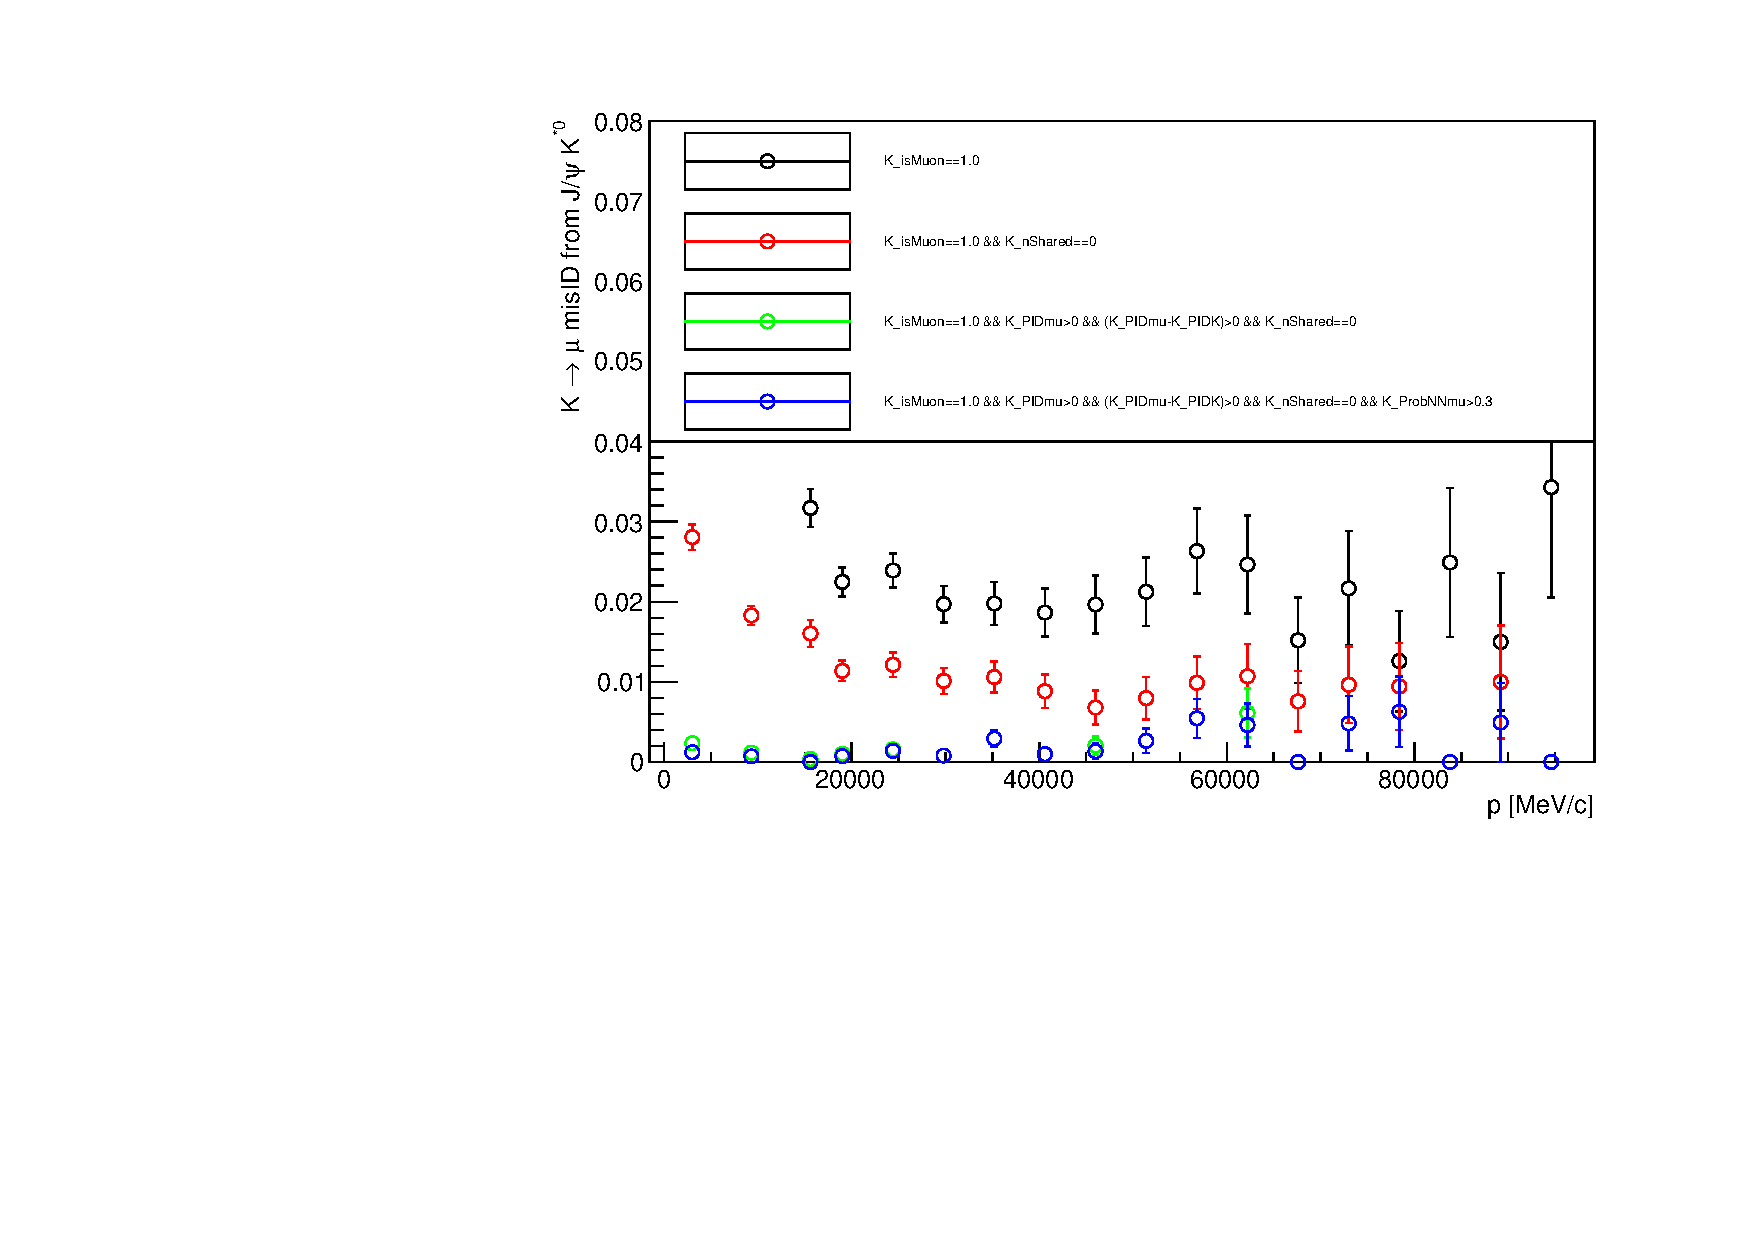
\includegraphics[width = 0.55\textwidth]{figs/trimuon/jpsikst/2012/Visualize_Weights_KaonMisid_2011_small.pdf}\put(-50,133){(a)}%
		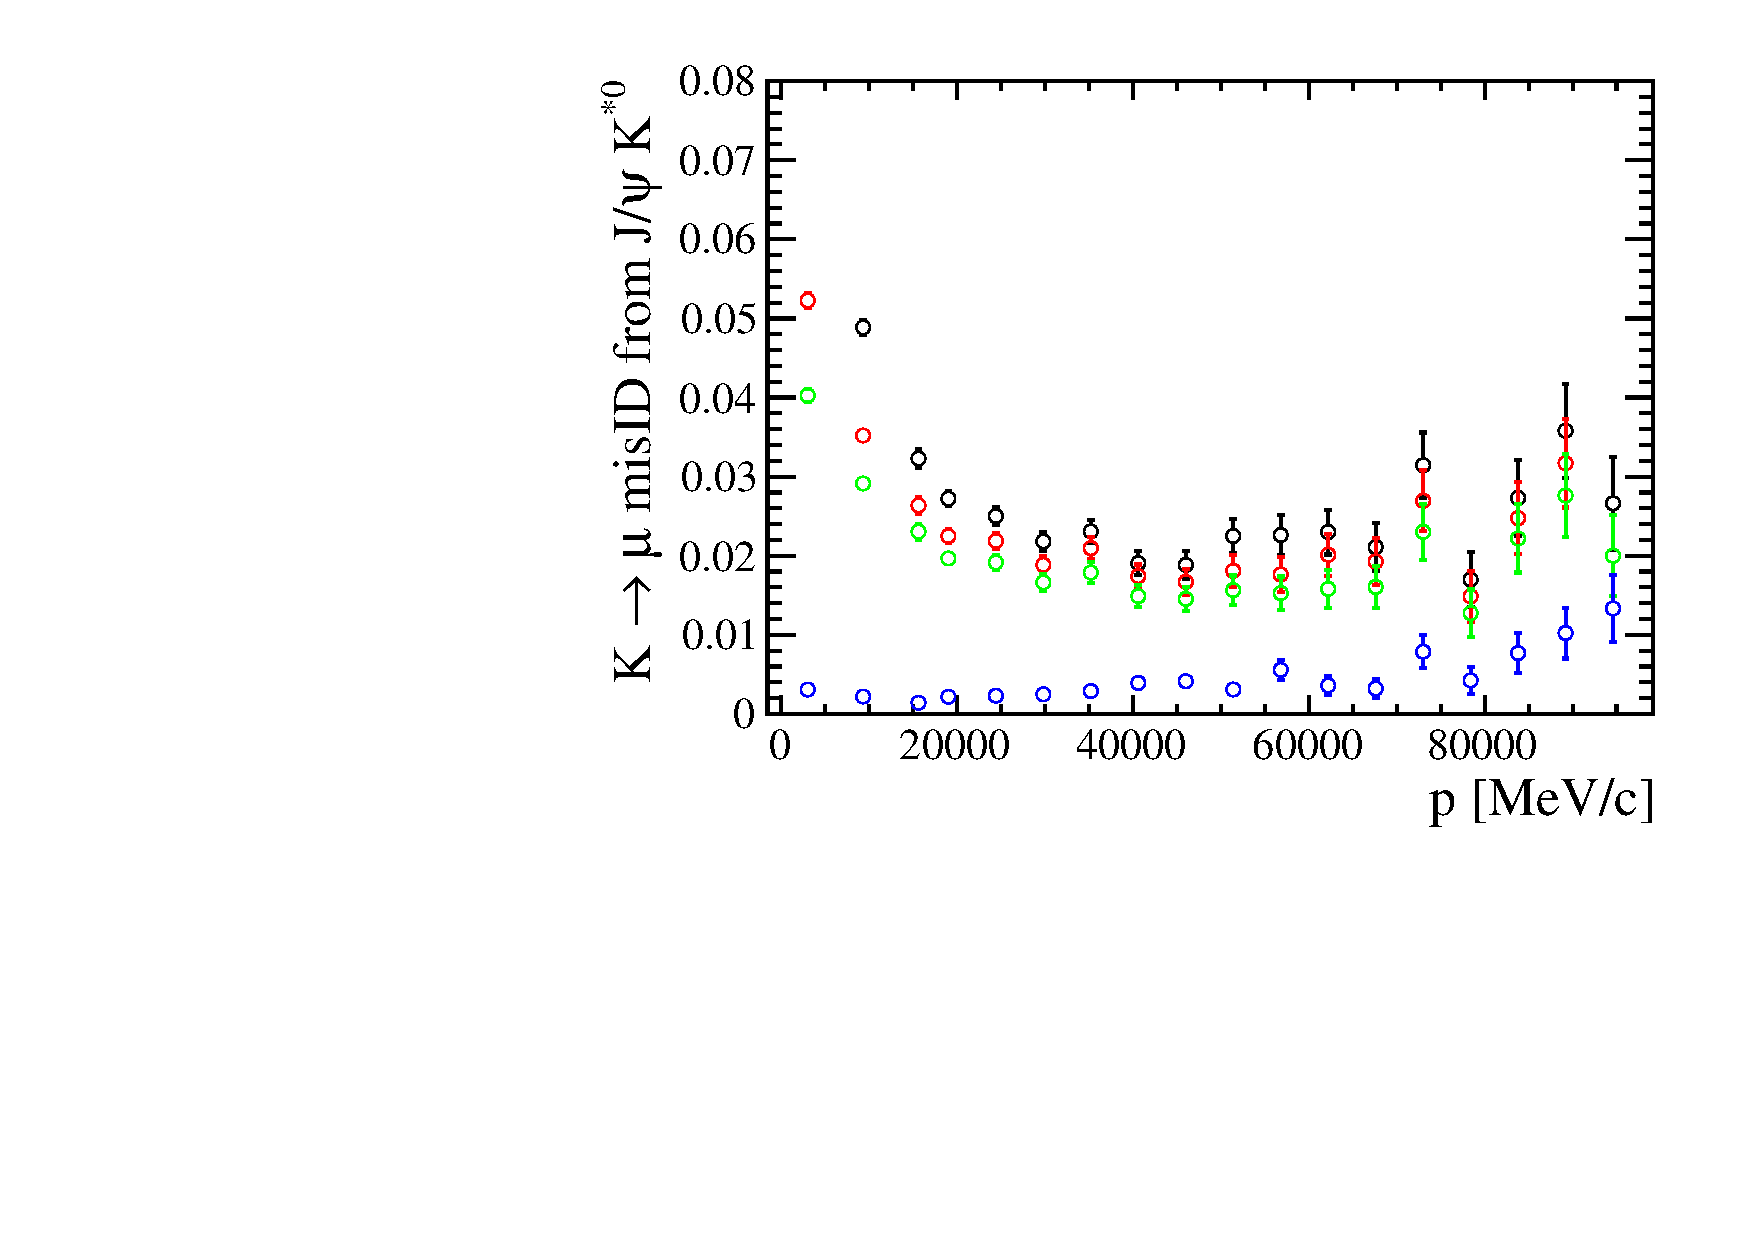
\includegraphics[width = 0.5\textwidth]{figs/trimuon/jpsikst/2016/Visualize_Weights_KaonMisid_2016_small_thesis.pdf}\put(-50,133){(a)}
%		\newline
%		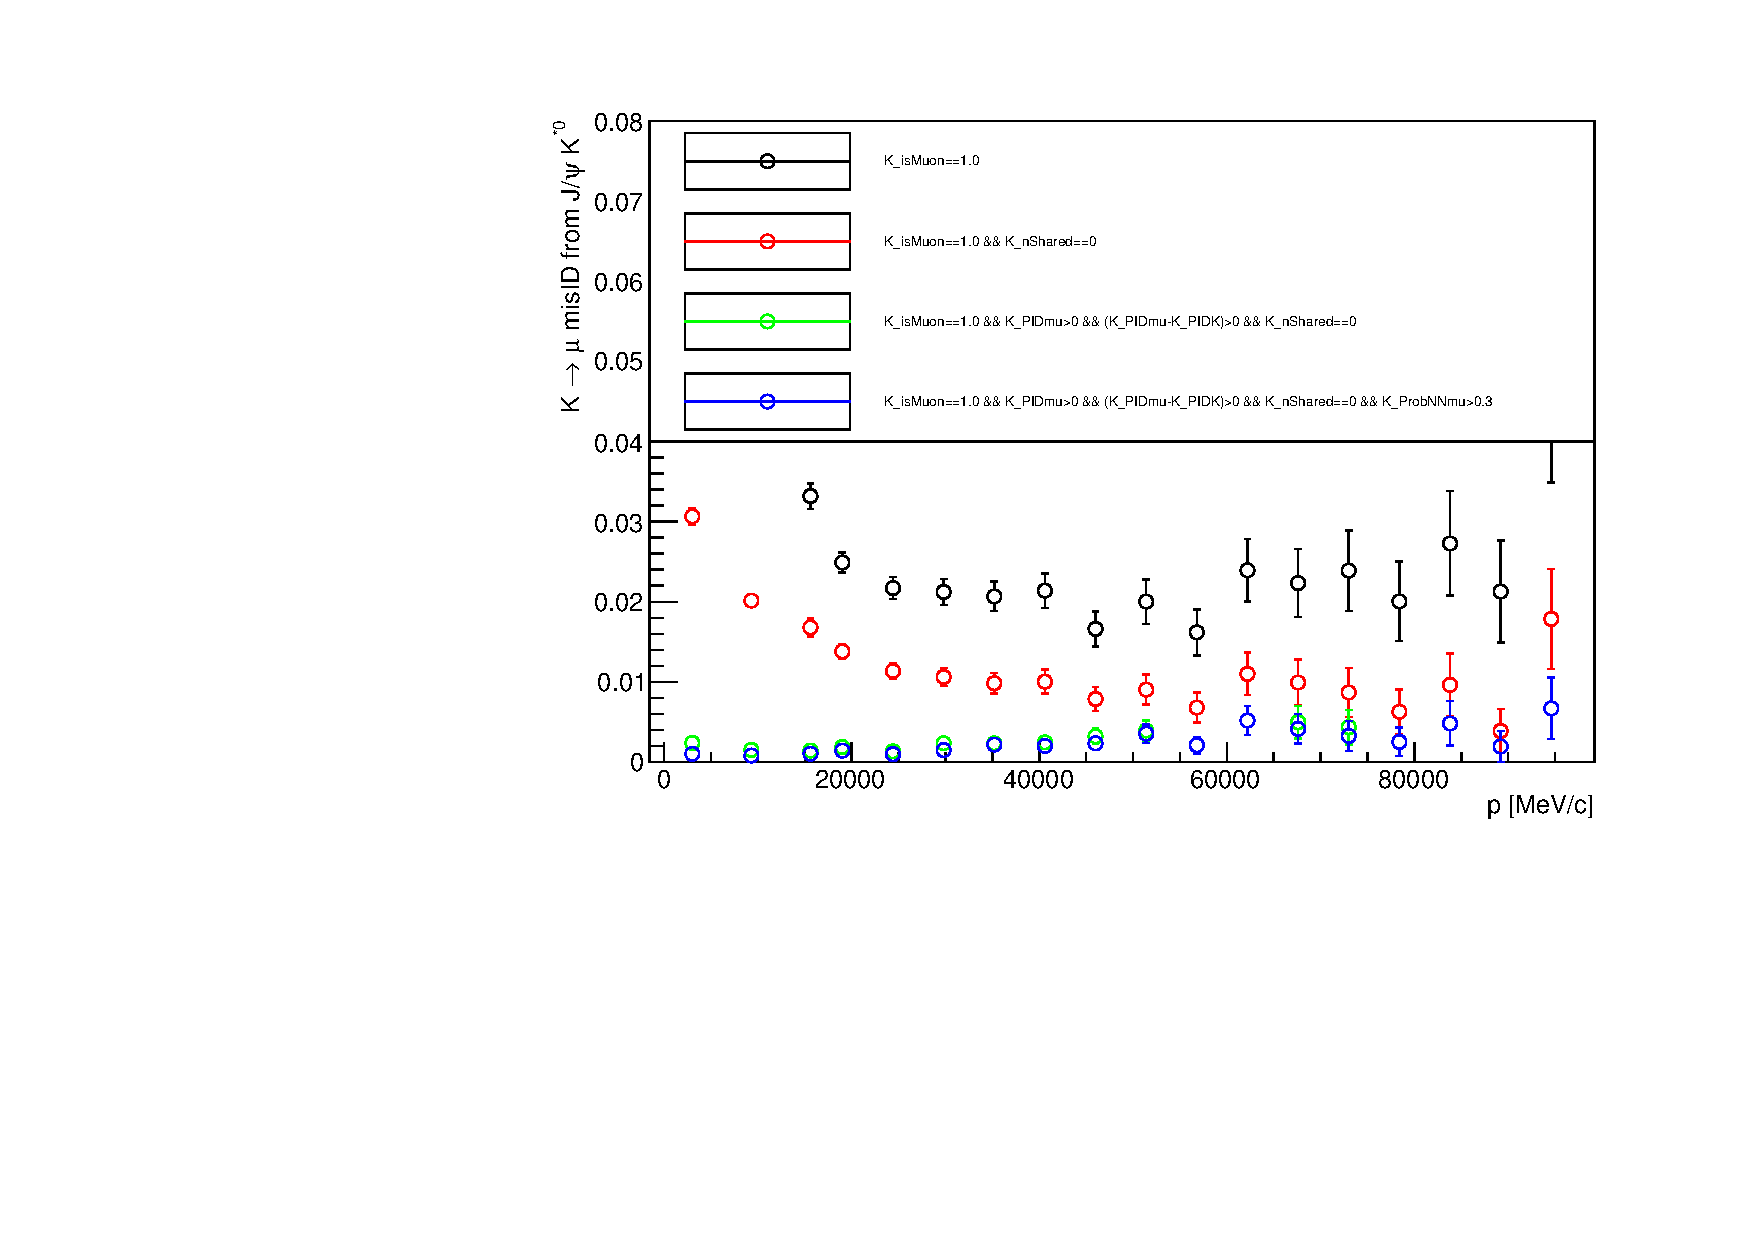
\includegraphics[width = 0.55\textwidth]{figs/trimuon/jpsikst/2012/Visualize_Weights_KaonMisid_small.pdf}\put(-50,133){(c)}%
		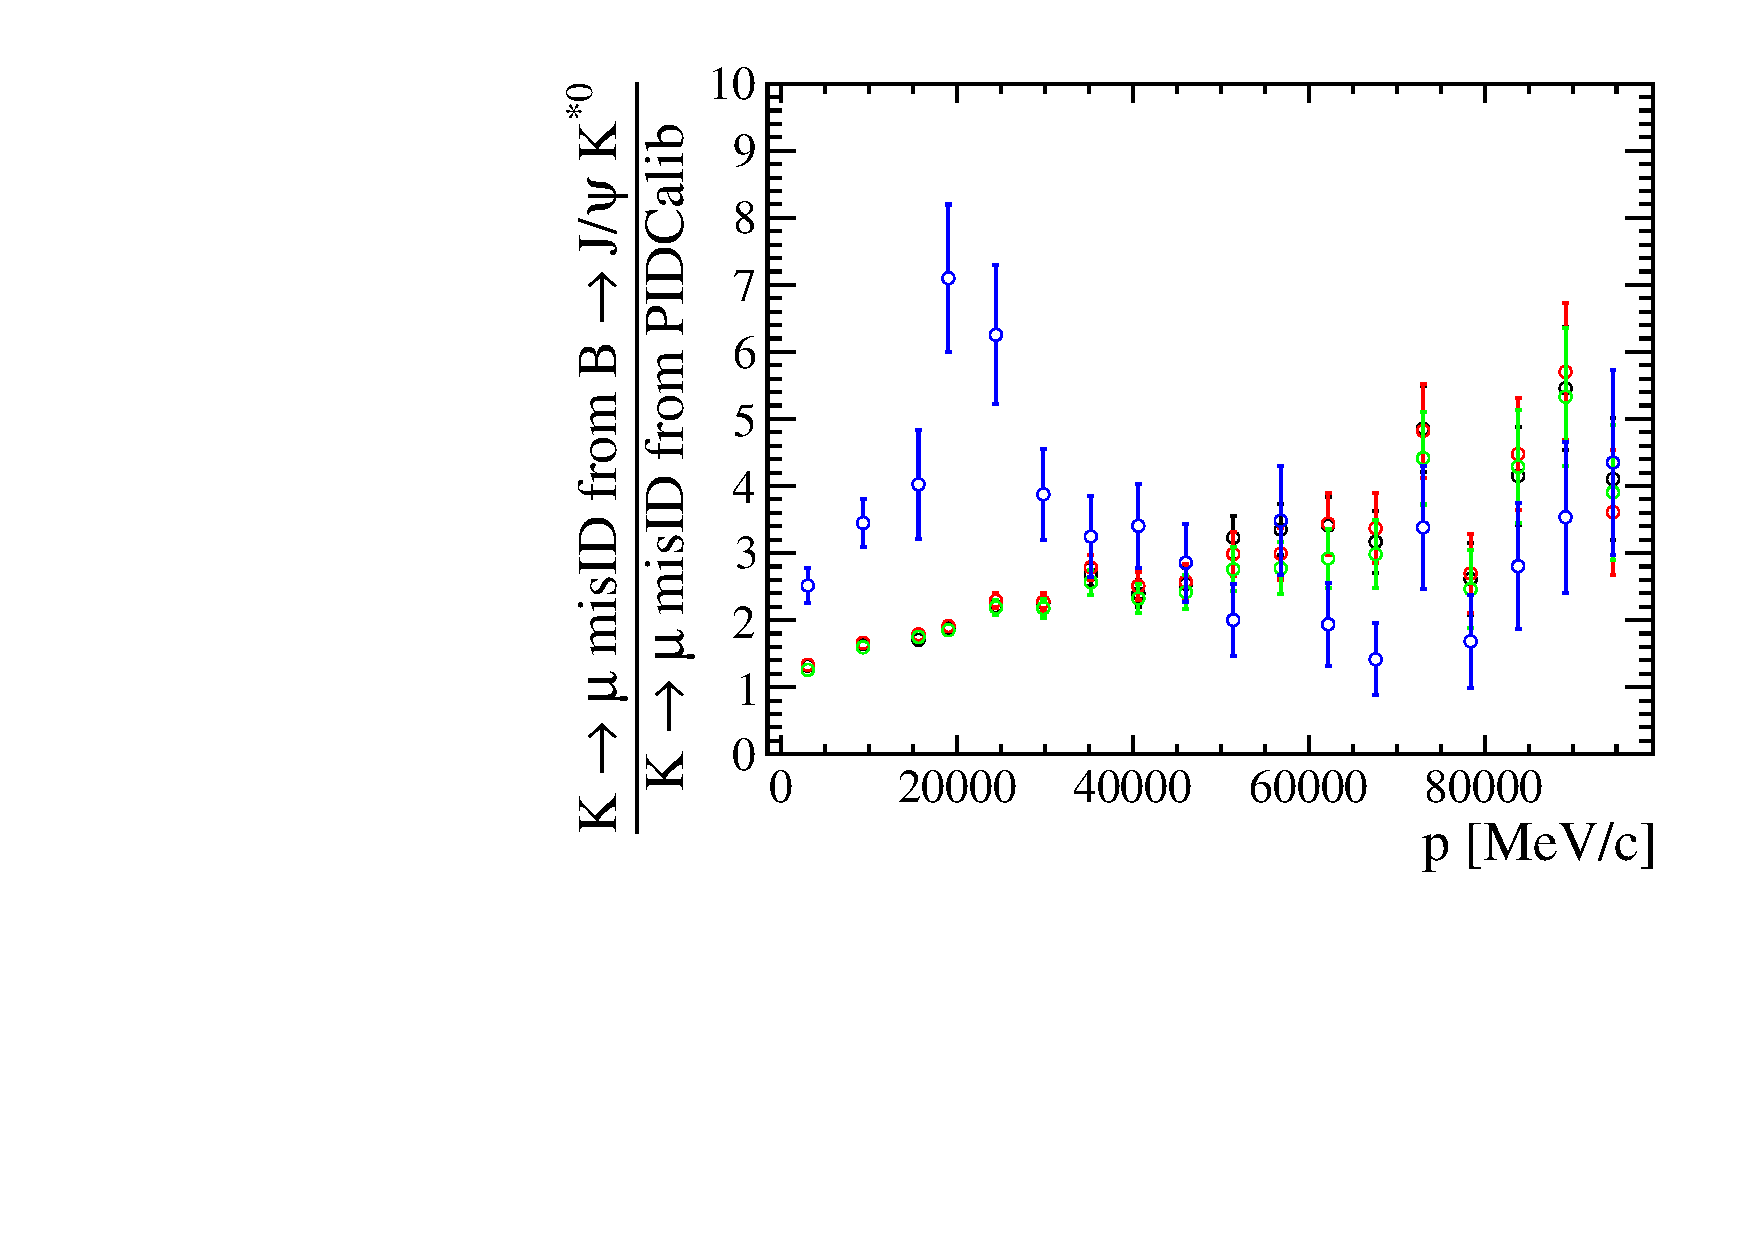
\includegraphics[width = 0.5\textwidth]{figs/trimuon/jpsikst/2016/Visualize_Ratios_2016_KaonMisid_small_thesis.pdf}\put(-50,133){(b)}
		\newline
%		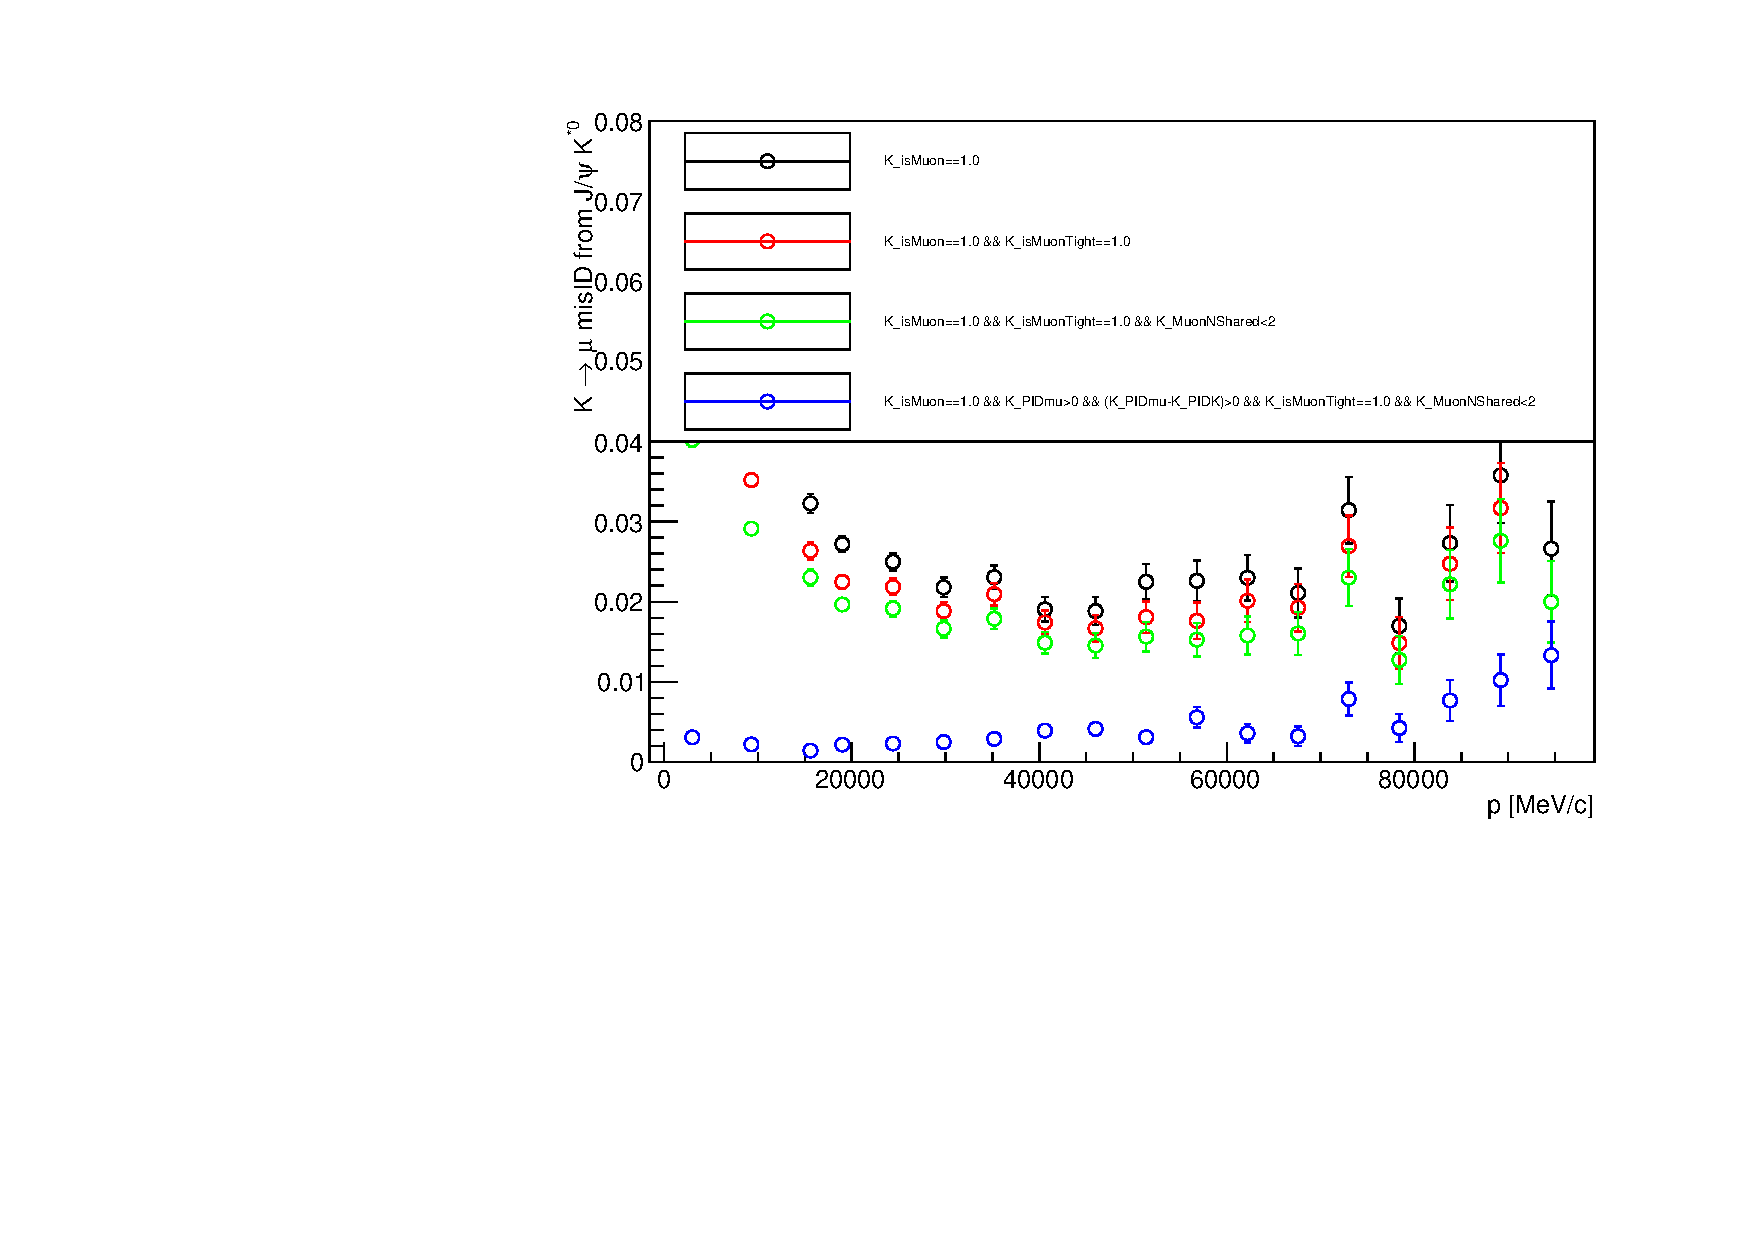
\includegraphics[width = 0.55\textwidth]{figs/trimuon/jpsikst/2012/Visualize_Weights_KaonMisid_2016_small.pdf}\put(-50,133){(e)}%
		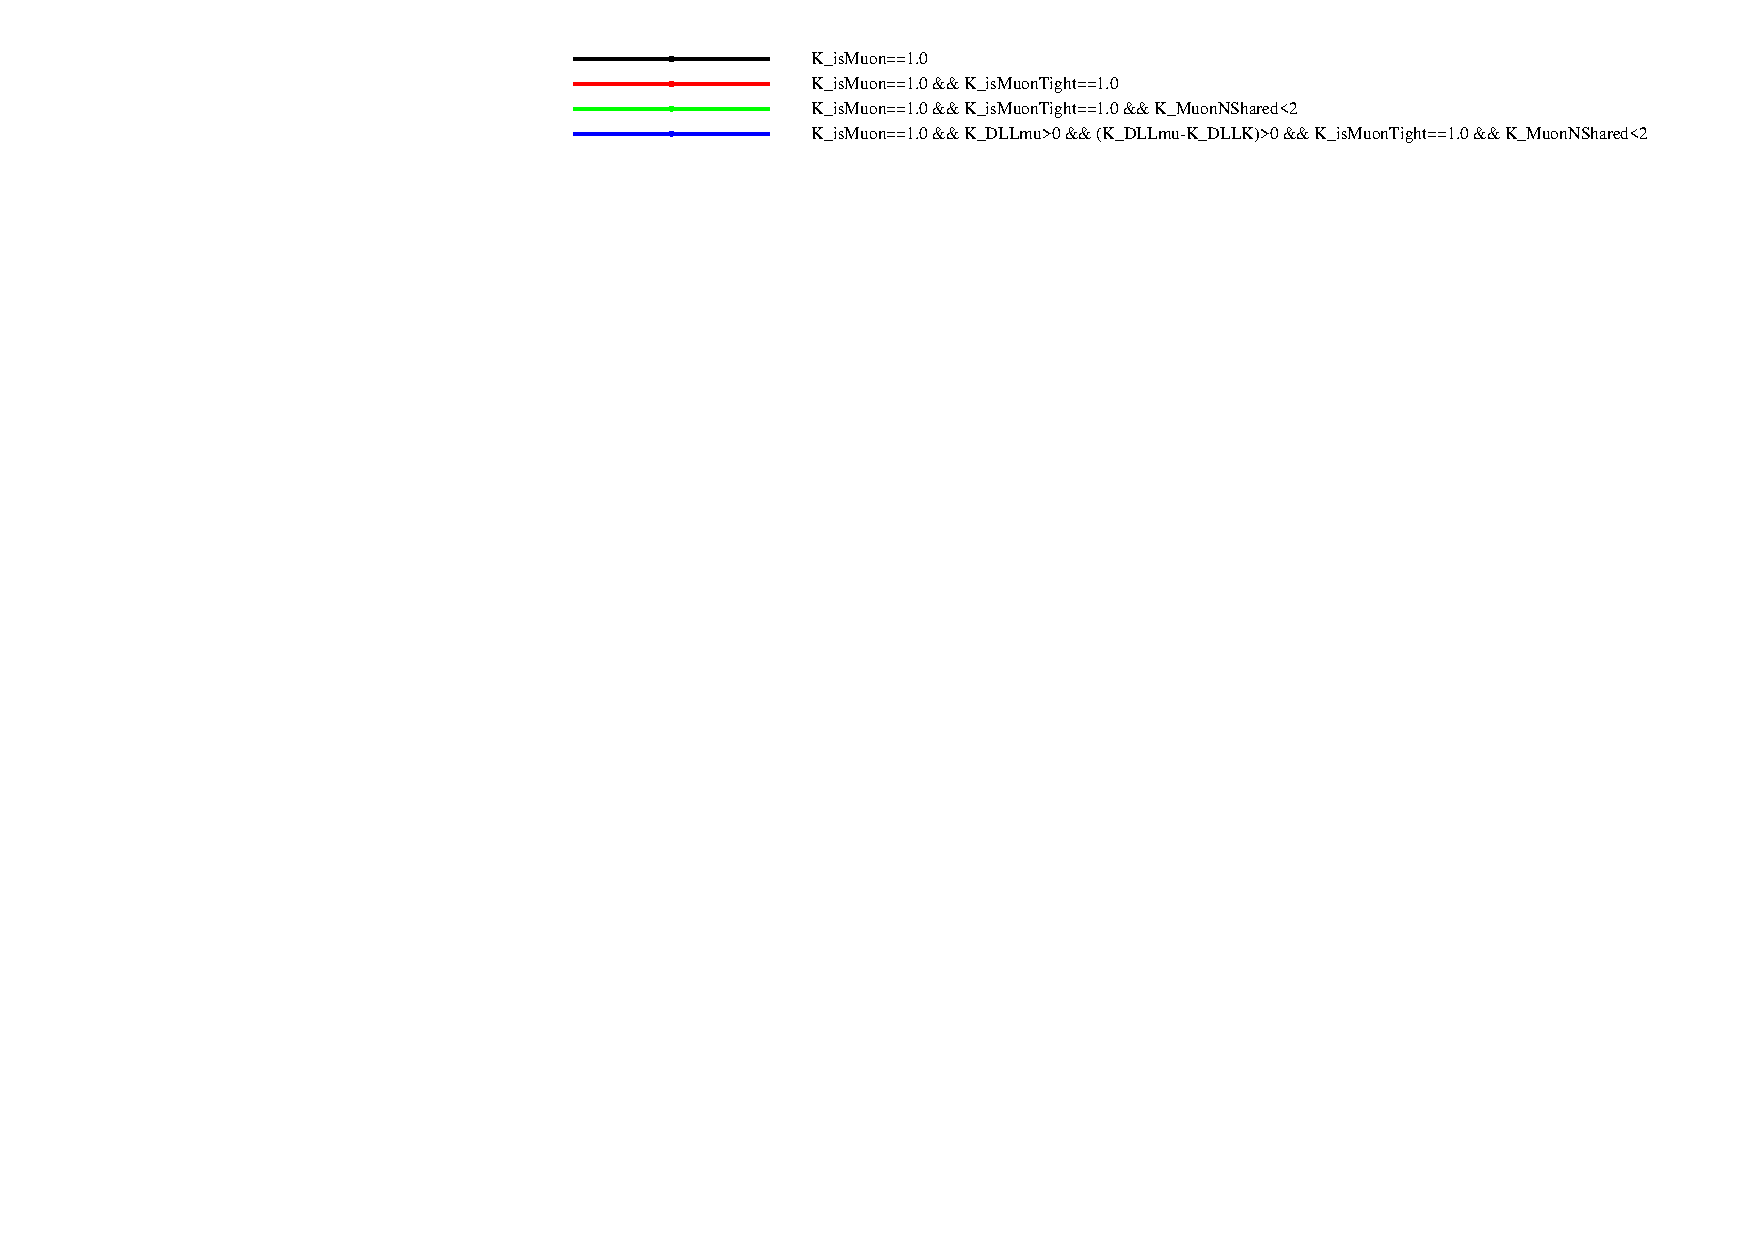
\includegraphics[width = 1.0\textwidth]{figs/trimuon/jpsikst/2016/Visualize_Weights_KaonMisid_2016_small_thesis_legend.pdf}
		\caption{(a) $K \rightarrow \mu$ misID probability for different PID requirements obtained using $B^{0} \rightarrow J/\psi(\rightarrow \mu^{+} \mu^{-}) K^{*} (\rightarrow {K^{+} \pi^{-}} )$ for 2016 data. (b) This is compared to the standard \texttt{PIDCalib} $D^{*+}(\rightarrow D^{0}(\rightarrow K^{+} \pi^{-}) \pi^{+})$ sample. }
		\label{fig:JpsiKaonnew2016}
\end{figure}


